%% \documentclass[sigconf,10pt]{acmart}
%% \documentclass[sigalternate,10pt]{acmart}
\documentclass{sig-alternate-10pt}

% Added packages
\usepackage{enumitem}
\setlist{leftmargin=5.5mm}
\usepackage{array}
\usepackage{booktabs} % For formal tables
\usepackage{xspace}
\usepackage{multirow}
\usepackage{makecell}
\usepackage{graphicx,amssymb,amsmath,endnotes}
\usepackage{ulem}
\usepackage{subcaption}
\usepackage{wrapfig}
\usepackage{fancyhdr}
\fancyhead{}
\fancyfoot{}
\fancyfoot[C]{\thepage}
\usepackage{textcomp, libertine}
% Copyright
% \setcopyright{none}
% \renewcommand\footnotetextcopyrightpermission[1]{}	% Remove this in camera ready
% \settopmatter{printfolios=true} 
% \settopmatter{printacmref=false}
\pagestyle{plain}
\normalem

\title{Verification: Feasibility of Self Constructive Component-Wise Power Modeling on Modern Smartphones}
\author{
Paper ID: , pages = 8+2
% Anonymous Author(s)
}


\newcommand{\oldstuff}[1]{}
\newcommand{\yes}{$\checkmark$}
\newcommand{\limited}{Limited}
\newcommand{\no}{$\times$}
% \definecolor{gray}{rgb}{0.5,0.5,0.5}
\newcommand{\etc}{{\it etc.}\xspace}
\newcommand{\etcc}{{\it etc.}}
\newcommand{\ie}{{\it i.e.,}\xspace}
\newcommand{\eg}{{\it e.g.,}\xspace}
\newcommand{\etal}{\emph{et al.}\xspace}
\newcommand{\SmallCrunch}{\vspace{-0cm}}
\newcommand{\smallcrunch}{\vspace{-0cm}}
\newcommand{\questionaj}[1]{{\it #1}}
\newcommand{\updated}[1]{{\it {}}}
%\newcommand{\updated}[1]{{\color{red} {updated: #1}}}
\newcommand{\editaj}[2]{{\sout{#1}\color{red} {#2}}}
\newcommand{\removeaj}[2]{{\color{red}{\textbf{Remove following:}}}{\sout{#1}}	{\color{red} {\textbf{Because} #2}}}
\newcommand{\addaj}[1]{{\color{red} {ADD?: #1}}}
%\newcommand{\highlight}[1]{{\color{blue}#1}}
\newcommand{\insitu}{{\em in situ}\xspace}
\newcommand{\name}{{\sc PFOP}\xspace}
\newcommand{\namee}{{\sc PFOP}}
\newcommand{\ychurm}[1]{{\hspace{-0.2cm}}}
\newcommand{\panic}[1]{\vspace{-#1 plus 1pt minus 1pt}}
\newcommand{\panictwo}[1]{\vspace{-#1 plus 2pt minus 2pt}}
% \newcommand{\nsection}[1]{\panictwo{0pt}\section{#1}\panictwo{0pt}}
% \newcommand{\nsubsection}[1]{\panictwo{0pt}\subsection{#1}\panictwo{0pt}}
% \newcommand{\nsubsubsection}[1]{\panictwo{0pt}\subsubsection{#1}\panictwo{0pt}}
\newcommand{\flow}{flow\xspace}
\renewcommand{\comment}[1]{{\it #1}}
\newcommand{\forjnl}[1]{{}}
\newcommand{\dcomment}[1]{{\color{blue} #1}}
\newcommand{\expr}[1]{{\color{red} Experiments: #1}}
\newcommand{\coflowone}{C_1}
\newcommand{\coflowtwo}{C_2}
\newcommand{\nexuserror}{19.4\%\xspace}
\newcommand{\pixelerror}{23.8\%\xspace}
\newcommand{\motoerror}{13.4\%\xspace}
\newcommand{\nexuserrorreduction}{5.9$\times$\xspace}
\newcommand{\pixelerrorreduction}{7.2$\times$\xspace}
\newcommand{\motoerrorreduction}{4.6$\times$\xspace}
\newcommand{\revv}[1]{{#1}}
\newcommand{\tabincell}[2]{\begin{tabular}{@{}#1@{}}#2\end{tabular}}
\newcolumntype{P}[1]{>{\centering\arraybackslash}p{#1}}
\renewcommand{\paragraph}[1]{{\vspace{0.1in} \noindent \bf #1}}

\newcommand*\rot{\rotatebox{90}}

\newcommand{\cut}[1]{{}}

\date{May 2020}

\begin{document}

\maketitle
\begin{abstract}

Power modeling of mobile device components is foundational to mobile app energy drain analysis such as energy profiling and energy debugging of mobile apps. Traditional power model derivation (TPMD) is an offline process based on microbenchmarks 
% to drive each mobile device component into each possible power state to record its power draw (from a power monitor) 
which cannot capture the power model's dependence on app usage, the mobile device and environment such as the battery age.
% or device temperature. 
Self-constructive power model derivation (SPMD) promises to overcome these shortcomings of TPMD by collecting 
% each actual power state that each device component ran under, the utilization, and 
component power state and utilization , total device energy drain during an app run and derives the power model parameters by regression using a system of linear equations. 
Though first proposed almost a decade ago, SPMD has only been explored so far for energy drain estimation with a finer resolution (e.g. 10ms) compared to the device power sensor readings (e.g. 1s). 


In this paper, we perform a verification study regarding 
the feasibility of SPMD in deriving component-wise power models 
for modern smartphones. Our study shows that SPMD faces a 
fundamental dilemma: it can only be used for the particular 
app scenario as even different scenarios of the same app result 
in different power models; on the other hand, when 
restricted to a particular app scenario, the system of 
equations lacks diversity when created at the second granularity, 
preventing the regression solver to generate meaningful model parameters.  
%  Finally, we show
% zooming into the millisecond scale in setting up equations can overcome the diversity problem 
% but the equation can be dominated by measurement noise, and further SPMD would not scale
% as a 1-minute app run would require solving thousands of systems of equations. 
Our study suggests that it is extremely challenging to derive component-wise power model parameters for modern smartphones using SPMD. 

\if 0
In this paper, we perform an in-depth investigation of the feasibility of SPMD in deriving accurate per-component power models for modern smartphones. 
 % We systematically explore the time-scale for setting up the system of equations, ranging from macro-scale (one equation per second), to micro-scale (two equations per rendering interval to exploit GPU Busy and Idle power states), to nano-scale (16 equations per rendering interval to explore diversity within each rendering interval.)
We find that while conceptually simple, in practice it is 
extreme difficult to create a system of equations that 
exhibit sufficient diversity which poses two challenges 
to the regression solver to generate meaningful per-component 
power model parameters: (1) lack of diversity in phone
component usage which leads to the rank of the equations 
(right-hand-side of equations) to be smaller than the number 
of unknowns (model parameters); (2) noise in energy drain 
readings (left-hand-side of the equations) which results 
in contradicting component usage and energy drain. Our 
experimental results suggest that while SPMD may be useful for
energy modeling which only requires a good fitting of the two 
sides of the equations, it remain not practical for deriving 
per-component power model parameters for use in mobile app 
energy drain analysis such as energy profiling and energy debugging. 

%   We believe that our  ndings can encourage further research and standardization e orts towards higher utilization of commercialized CIoT network infrastructures.
\fi
\end{abstract}
\pagestyle{plain}

\section{Introduction}
\label{sec:motivation}

\subsection{Background and Motivation}
\label{subsec:back}


% In this section, we provide a brief background and motivation for self-power modeling of mobile devices, and discuss the prior-art. 

% \subsection{Power Modeling of Mobile Devices}

Modern smartphones come with a wide variety of hardware components
, \eg CPU, GPU, WiFi and LTE NIC, and OLED display. To offer rich 
user experience, mobile apps running on the phone often utilize 
several of these components simultaneously, each of these 
drawing power contributing  to the overall total phone power draw.

Diagnosing and managing the power draw of smartphones using an external power monitor or the phone 
built-in power sensor  (available in most smartphones today)
are difficult as they can only measure the total phone power draw.
Power modeling is a technique that allows breaking down the 
total phone power draw to the power draw by individual components, 
and is the foundation for various mobile device power
management solutions such
as mobile software energy profiling~\cite{flinn:1999,shye2009into,zhang2010accurate,sesame:2011,pathak2012energy,appscope,ding2017gfxdoctor,facebookbatterymetrics}, energy debugging~\cite{ma2013edoctor,benerjee:2014}, and in-the-wild energy measurement~\cite{chen:sigm2015,androidbatterystats,androidvitals}.  

% A power model for each phone component captures the mathematical correlation between the {\it events} that {trigger} the usage of the component and the resulting component power draw; it is a function takes power events for a given phone component as input and outputs the estimated power draw for that component due to those events.
{
Each of the phone components can potentially be 
in different power states, drawing different amount of power. 
An empirical power model for a component captures the power 
draw while the component in each of the possible power state, known as  the {\em power model parameter}.
%
Once derived, a component’s power model can be used to estimate 
the energy drain of the component during the runtime of any app. 
This is achieved by collecting the duration (utilization) that 
the component spends in each power state during the app run 
followed by post-processing i.e summing up the product of 
each utilization  duration with its corresponding power draw from the power model.
}

\paragraph{Traditional Power Model Derivation}
\label{subsec:tpmd}
Traditional power model derivation (TPMD) is an offline, largely manual process. 
\if 0
It runs microbenchmarks on the phone to exercise the phone components 
in isolation to induce the power triggering events. The triggers 
associated with each component are captured along with the 
instantaneous power measured using an external power monitor 
or the built-in power sensor. Next, the power used by each 
phone component is isolated and the power model is derived 
by extracting the correlation between the triggers and the components’ power draw.
\fi
which consists of four major steps: (1) Enumerate all the 
power states a component can possibly enter; (2) develop 
microbenchmarks that drive the component into each of these 
possible power state; (3) run the microbenchmark while collecting 
the component power draw online; and (4) while offline processing, 
align the power draw timeline with the microbenchmark execution 
to find the power draw corresponding to each of the power states 
the component is running in. If a component cannot be exercised alone
, \eg the WiFi NIC cannot be exercised alone without packet 
processing in the CPU, the power model for the component needs 
to be derived incrementally (see \S\ref{sec:primer} for an example.)

Although conceptually simple, traditional power model derivation suffers several major drawbacks. 

\cut{ 
{\it (1) Labor-intensive manual process.}
First, TPMD is a laborious process that faces many practical challenges:
(1) Connecting an external power source to a commodity phone is challenging.
\cut{The technique requires a soldering station and the skill to disassemble 
the device and solder the power monitor wires to the power management circuit.
}
% For example Moto Z3 and Nexus6 have different arrangements.
%i.e Nexus6 only the back cover has to be removed and probes are connected whereas Z3 requires the total disassembly and removal of the battery.
(2) The entire process is time consuming.
For example, the CPU of the Moto Z3 phone released in August 2018 comes with 8 cores, and
the 4 LITTLE cores can be dynamically adjusted among 22 frequencies 
and the 4 big cores can be adjusted among 31 frequencies. 
To derive the CPU model, a benchmark is run at each core at each CPU frequency 
% with 100\% CPU utilization
for a certain duration and the process is repeated for all the big.LITTLE core-frequency combinations.
Some of these frequency combinations may never appear in a real app run.
% This cumbersome process inhibits researchers from developing power models for diversity of phones.
}


{\it (1) App usage dependence.}
{The most serious drawback of offline power model derivation 
using microbenchmarks is the modeling error 
from not able to capture {\it power state variations} for any particular app execution.  
}
A power state variation for a component happens when different 
functional units inside the component may be exercised under different 
app usage. As a result, the amount of power the component draws varies  . 
An example of this is while the CPU is running in the same frequency with  100\% utilization, 
integer arithmetic workload and float arithmetic workload can lead to 13.5\% 
different CPU power draw running at 2.45GHz on Moto Z3.
The number of possible power state variations can also be unknown or simply 
too many to enumerate.

\if 0 
\cut{ 
TPMD assumes all the exact power states for each component are known and are modeled during offline model derivation. In practice, this is hard do for several reasons:
(1) there can be power state variations that the microbenchmark author may not be aware;
(2) the number of possible power state variations can be too many and hence too expensive to enumerate;
(3) enumerating all possible power state variations may not be
necessarily useful as many combinations of power state variations 
(of different components) may not appear in real apps.
%
% (3) logging all triggers can be prohibitively expensive or not allowed by the OS. 
%  In practice, there are possible hidden triggers not captured in the power models  which may be exercised differently by different apps~\cite{dong2011self}. 
For these reasons, the offline-derived power models 
may not be able to model all power state variations and hence
may not capture the actual component power draw behavior during a particular app run
which can lead to significant model error. 
}
\fi 

{\it (2) Device and environment dependence.}
In addition, power models are phone-specific and hence the TPMD process needs to be repeated,
\eg by an OEM phone vendor for all its phone models. 
Furthermore, even two devices of the same model can have different 
power models depending on the age of the device and effect of 
external factors such as phone temperature.These factors require 
the power models to be re-derived.

\paragraph{Self Power Model Derivation}
\label{subsec:spmd}
%
Self power model derivation (SPMD)~\cite{dong2011self} promises to overcome 
the app usage/device/ environment dependencies of TPMD. 
Instead of developing and running microbenchmarks to drive the 
phone component into each of the possible power states including 
power state variations, SPMD collects details of each of the 
actual power state that each phone component ran under, the 
utilization (duration) in it, and the total phone power draw 
using the power sensor or power monitor  during each actual 
app run. In post-processing SPMD sets up and solves equations 
that express the total phone energy drain for each of the time 
interval as the sum of energy drain for all the components which 
are linear functions of component power draws
, \ie each model parameter multiplied by the corresponding utilization.

Thus SPMD is "in-situ"; the component power models are generated 
at the end of each app run and hence SPMD avoids the time-consuming 
offline model derivation in TPMD.
Second, SPMD is intrinsically phone specific and handset specific, 
and adapts with environment factors that can affect component power 
draw such as the battery age and phone temperature. 
Finally, SPMD is intrinsically specific to
the app run and hence the relevant phone component usage and power 
draw scenario. As such,
{it captures only the relevant power states that contribute to each 
phone component power draw during specific app run.} 
These intrinsic handset, environment, and app specificities make SPMD 
likely to generate more accurate power models than TPMD; the 
derived model  even if may not contain all possible model parameters 
but it will contain all the required model parameters needed to analyze 
the energy drain of that particular app run. 


\if 0
The power consumed by a smartphone heavily depends on its hardware components and configurations.
Due to it's nature, traditional power modeling provides fixed models.
Different apps uses various hardware components to a varying extent with inter-component interactions, which may not be modelled by a fixed power model.

As self modeling is done on device, it is inherently environment agnostic and leads to accurate power modeling.

\fi



\paragraph{Prior Work: Sesame}
\label{sec:back}
%
Sesame~\cite{dong2011self} was one of the first work to demonstrate 
the feasibility of self power model derivation.\footnote{We distinguish SPMD from self-metering work such as~\cite{zhang2010accurate,devscope:2012} 
which used built-in battery interfaces to measure the power or 
use regression but still used training microbenchmarks to 
exercise one phone component at a time.
% and hence the models derived are not app usage agnostic.  
}
% Few application of modelling as stated in Sesame could be detecting rogue applications and adding support to OS for determining adequate measures in optimizing battery life in a classical way.
% Various  models developed in  classical way are also influenced by the variable internal resistance of the device battery.
% Sesame also mentions that traditional energy models of 1 Hz are fundamentally inadequate for applications such as per-application energy accounting.
% Sesame idea is to devise a model molding method that achieves high accuracy and high rate when combined with principal component analysis and to realize Sesame on resource-limited mobile devices (as it is impractical to include all predictors that can account for every hardware detail because not all hardware components are visible to the OS and collecting the values of a large number of predictors would incur significant overhead).
However, its motivation and design goals were not on constructing 
{\it component-wise} power models. Instead, its primary goals were (1) modeling the whole phone energy drain at a higher rate, \eg 100 Hz,
than what the built-in power sensor could provide, \eg 1Hz, and (2) doing so without external high-resolution power monitors so the model could be "personalized" for a given app on a given device.  
% The primary motivations of Sesame are (1) to improve model accuracy by eliminating the model dependencies on hardware, app usage and battery conditions; and (2) to ease model derivation by automatically generating energy models without external assistance.
%    \item Utilize real usage of every individual user to generate personalized energy models and to adapt % such models for potentially higher accuracy
%
\if 0
However, though Sesame~\cite{dong2011self} pioneered the concept 
of self power modeling, the study which was conducted over a decade 
ago had two major limitations.
First, it focused on fine-resolution whole-phone energy drain 
estimation, \eg the total phone energy drain at fine-resolutions, 
as opposed to per-phone-component power or energy drain estimation.
\fi 
In particular, it uses battery State-of-Charge (SoD) readings to 
set up the energy drain equations at the power sensor sampling 
resolution (\eg 1s), and uses the solutions to the unknowns to 
directly estimate the total energy drain at finer time-scales, \eg 10ms.
The work did not study the accuracy of component power parameters derived.

% However it is important to note that Sesame can incorporate any predictor that can be acquired in software. Sesame further utilizes the Advanced Configuration and Power Interface (ACPI) available on modern mobile systems.
% ACPI provides platform-independent interfaces for the power states of hardware, including the processor and peripherals.
% {\bf Device Used\\}

\cut{ 
Further, the study was on an early phone that had much simpler components
each with far fewer power states than those in modern smartphones. 
In particular, the Nokia N900 phone used had a single-core CPU and a low-end GPU by today's standards,
and either the CPU or the GPU could only run in a single  frequency.
Sesame models CPU, memory, WiFi, flash disk, and display; the GPU was not modeled. 
For a set of 3 benchmarks. % 9 apps,
Sesame achieved an average accuracy of 86\% when generating 1 energy drain estimation per second and 82\% at 1 estimation per 10ms against external power monitor measurement.
% {their abstract says 95\% and 88\%?. These number are for the T61 laptop. They used a laptop and phone for the evaluation.}
}



\input contribution

% ~\cite{eprof,androidprofiler}. 

\if 0
They used an full utilization model for there analysis~\cite{economou2006full}~\cite{ranganathan2007simulating}.
The model looked like
\begin{equation}
    Energy_{Total} = c_{o} + \sum{ c_{component} * u_{component}}
\end{equation}
The total energy is the sum of each component, with each having it own energy coefficient $c_{component}$.
They collected predictors from the OS to capture the utilization of components.
They used principal component analysis coupled with a linear regression solver to generate the energy model.
%{\bf Conclusion\\}
\fi



% \input{background}
%\comment {
\section{Why only CPU and GPU are considered?}
\label{sec:twocomponent}
As we have stated in~\S\ref{sec:motivation} modern smartphones have many components built into it.
We observe the contribution of CPU, GPU, network, media decoder power components in MotoZ3 for 10 popular Google Apps with more than 1 billion plus installs.
The findings for these apps are shown in table~\ref{tab:muti_component_analysis}.
We observe that the solution with four components is not converging.
So we choose only CPU and GPU, which are major components assuming that we can successfully model these two components and further extend it to cater more components.

\begin{table}[]
    \centering
    \caption{SPMD for 10 popular Google Apps with CPU, GPU, network and media decoder}
    \vspace{-0.1in}
    \begin{tabular}{|c|c|}
        \hline
         App &  \\
         \hline
          Google Calculator & \\
          Google Calendar & \\
          Google Chrome & \\
          Google Maps & \\
          Google News & \\
          Google Photos & \\
          Google Playstore & \\
          Google YouTube & \\
          Gmail & \\
         \hline
    \end{tabular}
    \label{tab:muti_component_analysis}
    \vspace{-0.1in}
\end{table}
}
%\section{Power Model Dependency on App Usage - A TPMD Study}
\section{At What Granularity of App Run to Apply SPMD?}
\label{sec:primer}

Since SPMD is meant to capture the power model's dependence on app usage, it should be applied to 
each app run interval that exhibits the {\em same} component usage.
To gain insight into the extent of such "same" component usage intervals of apps,
we start with a study to find out  how much the GPU power models derived using TPMD vary with
apps and app scenarios. 
% show the component power draw dependency on app usage 
% using a representative modern phone, Moto Z3,
% by performing TPMD to generate the CPU and GPU power models
% on a representative modern phone, Moto Z3.
% In particular, we discuss the four-step process of TPMD discussed in \S\ref{sec:back} for the CPU and the GPU.
For the experiments in this section,
we use the external Monsoon power monitor ~\cite{monsoonpowermonitor} to measure the phone power draw.
We keep the screen brightness level at 0 which consumes 51.38 mA and this is subtracted
from the total phone power draw measurement.

\begin{table}[t]
{\footnotesize
    \centering
    \caption{CPU and GPU power model parameters on the 3 phone. (PF: per frequency.)}
    \vspace{-0.1in}
    \begin{tabular}{|c|c|c|c|c|}
         \hline
         Model Parameters & Parameter  & \multicolumn{3}{c|}{Number of Parameters}\\
         \cline{3-5}
          & Symbol & Pixel 2 & Moto Z3 & Pixel 4\\
         \hline
        CPU base power                          & $p^c_{base}$          &  1      &   1       & 1\\
        CPU core $i$ power at freq. $f_k$       & $p^c_i(f_k)$          & 31, PF  &  31, PF   & 17, PF\\
        % TODO: add per frequency per core in the description\\
        GPU busy power at freq. $g_k$           & $p^g_{busy}(g_k)$     &  7, PF  &   7, PF   & 5, PF\\
        GPU idle power at freq. $g_k$           & $p^g_{idle}(g_k)$     &  7, PF  &   7, PF   & 5, PF\\
         \hline
    \end{tabular}
    \label{tab:parameters}
    \vspace{-0.1in}
}
\end{table}

% \questionaj{We need a paragraph here (perhaps reference table 3?) detailing which 
% trigger are we logging, where are we logging them from, and is experiment done 
% using power monitor or power sensor

\if 0
Power models for mobile devices have been actively studied in recent years, and the proposed power models fall into two major categories.

The first category of power models known as utilization-based models for smartphones (e.g., [21, 24, 25]) are based on the intuitive assumption that the utilization of a hardware component (e.g., NIC) corresponds to a certain power state and the change of utilization is what triggers the power state change of that component. Consequently, these models all use the utilization of a hardware component as the “trigger” in modeling power states and state tran- sitions. Such models thus do not capture power behavior of modern wireless components that do not lead to active utilization such as the promotion and tail power behavior of 3G and LTE [19, 12], and thus can incur high modeling error.
The second category of power models capture the non-utilization- based power behavior of wireless components using finite state ma- chines (FSMs), e.g., [8, 15, 18, 16, 17, 9] for WiFi and 3G and [12] for LTE. In a nut shell, the built-in state machine of the wire- less radio, e.g., the RRC states and transitions in LTE, is reverse- engineered and represented in a finite state machine that annotates each power state or transition with measured power draw and dura-
\fi



\if 0
\subsection{Power Model for Modern Smartphones}

The modern smartphones have came a long way, with different components which are capable of running in various power states.
This calls for a complex power model, in comparison to the pure utilization model.
We focus our attention in exploring per-component self-modeling of smartphone using CPU and GPU.
The decision of modeling only CPU and GPU was taken due to the fact that these are major energy consuming components in a modern day smartphones.

\fi
%%% Need to justify with a profiled data

% However earlier paper ~\cite{Zhang2015self} 
% observe  that this
% assumption does not hold good for multicore CPUs in modern smartphones. Even under the same frequency and
% CPU utilization, two workloads with different CPU usage patterns could
% consume significantly different amounts of energy
% The root
% cause of the estimation inaccuracy and instability come
% from multiple newly introduced CPU idle power states,
% which consume markedly different amounts of power in
% multicore CPUs. Workloads with different CPU usage
% patterns cause CPU to enter different idle power states
% during the computation, which in turn leads to different amount of CPU power consumption.

%\subsection{CPU Power Model is App Dependent}
\label{sec:primer_cpu}

%%% Things discussed in this section
%% 1. Explain the CPU architecture
%% 2. Explain how memory operation effects CPU model
%%   2a. Description of benchmark
%%   2b. What we did
%%   2c. Explanation of results
%% 3. Explain how CPU model is derived and generated
%%   3a. What did we do
%%   3b. How model is derived
%%   3c. Explain Base Current and Non-Base Current
%% 4. Explain the complete model

\paragraph{Parameters of a multicore CPU power model}
% 1. Explain the CPU architecture
Moto Z3~\cite{motoz3} is a representative modern smartphone
that uses the big.LITTLE CPU architecture~\cite{biglittlearch} to
provide energy efficiency in supporting diverse workloads.
% In this architecture, the CPU has two core clusters,
% the LITTLE cores with low compute performance and high power efficiency and
% big cores with high performance for processing compute-intensive tasks.
%The use of big.LITTLE cores depends on the dynamic usage pattern of smartphones i.e. when the phone is not working on doing any computationally intensive tasks it switches to LITTLE cores, dramatically extending the battery life.
% The cores in each cluster can run at various frequencies which correspond to 
% different core power states draining different amount of power.
In particular, in Moto Z3, the LITTLE cores can operate in 22 frequencies 
and big cores can operate in 31 frequencies.
%  The cores are switched to higher frequencies when higher performance is required.
At runtime, the OS scheduler along with the CPU governor performs power state transition and core frequency scaling to optimize the CPU energy drain as the workload varies.

Thus the parameters of the CPU power model include
the base power consumed $p_{base}$ when the cores are idle and
the non-base core $i$ power running at frequency $f_k$, $p^c_i(f_k)$, as listed in Table~\ref{tab:parameters}.
The total CPU power can be modeled~\cite{multicoremodel:2015} as follows:
\if 0
Accordingly, we model the CPU power draw as follows:
\begin{equation}
    P_{CPU} = p^c_{base} + \sum_i p^c_i{f(i)}
\end{equation}
where $p_{base}$ denotes the base power consumed when the cores are active and
$p_i{f_k}$ is the non-base power of core $i$ at frequency $f_k$.
\fi
{
\begin{equation}
    P_{CPU} = p^c_{base} + \sum_{i} p^c_i(f_k)
\end{equation}

}

\paragraph{TPMD methodology}
%% Flow of section
% 3. Explain how CPU model is derived and generated
%% 3a. What did we do
To derive the above CPU power model for Moto Z3,
we wrote a microbenchmark program that performs arithmetic-operations for 7 seconds at 100\% utilization followed by memory operations for 7 seconds at 100\% utilization. 
We ran the microbenchmark 10 times while fixing the big core cluster at each of the 31 frequencies, 
on 1 core, 2 cores and 4 cores.
When using 1 core, 2 cores and 4 cores, the remaining cores are offline.
We measure the base CPU power as the phone power draw when all cores are idle.
\footnote{We noticed even when the phone is idle, there are many system processes running in the background.
% 
So we obtained the accurate
base power from extrapolating the measured current vs. utilization curve for each frequency.}
We manually align the power monitor readings with each 7-second interval, 
and derive the non-base per-core power for each frequency by 
subtracting the base power from the measured total phone power.
{On Moto Z3, the per-core power $p_i(f_k)$ remains the same for different cores.}



% panab, check this ---
% The base CPU power is the current at utilization 0 and obtained from extrapolating the measured current vs utilization curve for each frequency.
% The non-base per-core CPU power for each frequency is the slope of the curve as shown in figure~\ref{fig:cpu_model_derivation}.

% at each big frequency.
% Little cores are offline
% Explain observations of microbenchmark

\if 0
\begin{figure}[tp]
    \centering
    \vspace{-0.1in}
         \begin{subfigure}[b]{0.49\columnwidth}
         \centering
         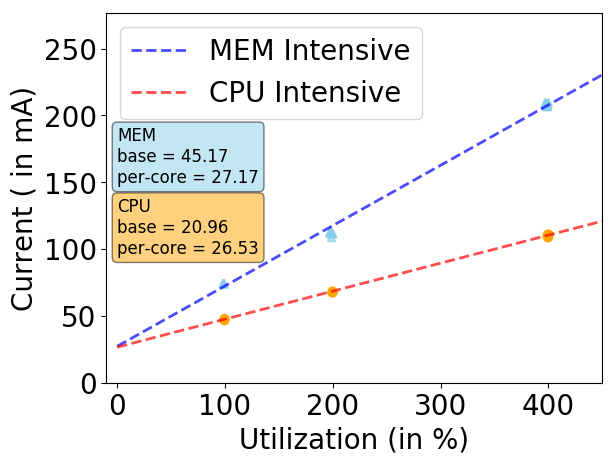
\includegraphics[width=\textwidth]{figures/576000.png}
         \caption{576 MHz}
         \label{fig:cpu_576000}
    \end{subfigure}
    \hfill
    \begin{subfigure}[b]{0.49\columnwidth}
         \centering
         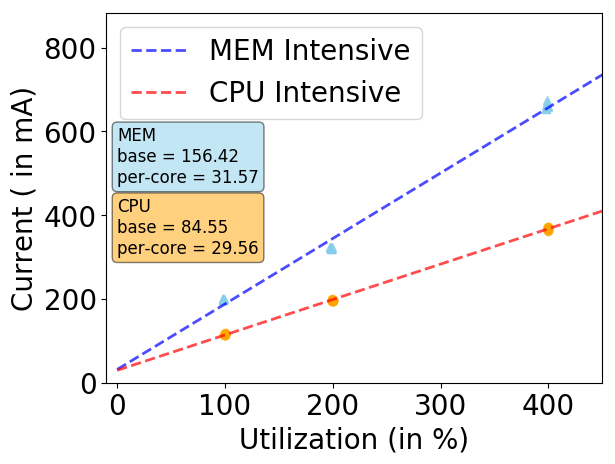
\includegraphics[width=\textwidth]{figures/1728000.png}
         \caption{1.728 GHz}
         \label{fig:cpu_1728000}
    \end{subfigure}
    \caption{The CPU derivation for two frequencies, 576 MHz and 1.728 GHz.}
    \label{fig:cpu_model_derivation}
    \vspace{-0.1in}
\end{figure}
\fi


\if 0
Figure~\ref{fig:cpu_model_derivation} shows 
the power consumed as a function of the CPU utilization for 576 MHz and 1.728 GHz,
for the two CPU benchmarks.
% While the blue line represents memory-intensive microbenchmark, red represents arithmetic-intensive microbenchmark .
% Figure~\ref{fig:cpu_576000} and~\ref{fig:cpu_1728000} corresponds to  576 MHz and 1.728 GHz
% Figure~\ref{fig:cpu_model_derivation} shows the power (averaged over 10 runs) linearly correlates with the utilization.
%% 3b. How model is derived
% We thus apply a regression-based solver to derive the best fit the following CPU power model:
% For each of the 31 frequencies, we derived a base and a per-core component with the following CPU power model.
% \begin{equation}
%     Power_{CPU}(f) = p_{base} + p_{f}*Utilization
% \end{equation}
% Where $p_{base}$ denotes the base power, and $p_{f}$ is the non-base per-core power running at frequency $f$.
%% 3c. Explain Base Current and Non-Base Current
For each of the 31 frequencies, we derived both base power and per-core component power.
We also observe that a reliable model can not be generated for the higher range of frequencies, like for frequencies higher than 2.035 GHz on MotoZ3 observations become unstable for CPU benchmarks.
The valid sets of base and per-core power were used for CPU modeling.
We observed that the base power is independent of frequency and per-core power is dependant on frequency.
Base power is 27.85 mA with a standard deviation of 1.22 mA.
% 
% We know the cores those are running at the 100\% utilization and remaining cores are offline.
% So, we can equate the number of running cores with utilization.
% We also observe that a reliable model can not be generated for the higher range of frequencies, like for frequencies higher than 2.035 GHz on MotoZ3 observations become unstable for CPU benchmarks.
% Fortunately, the apps rarely require these higher CPU frequency states and for our investigation we don't require those coefficients.
% \comment{stdev of what? fitting error on whole equation?}
% \comment{what is the following trying to say?}
During a  real run various cores may run on various frequencies.
\fi

\begin{figure}[tp]
    \centering
    \vspace{-0.1in}
         \begin{subfigure}[b]{0.49\columnwidth}
         \centering
    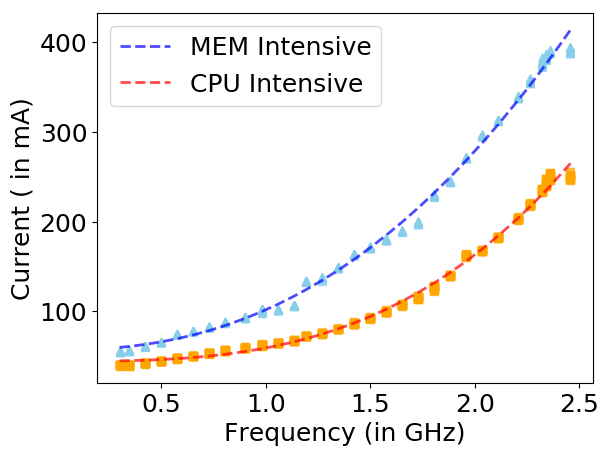
\includegraphics[width=\columnwidth]{figures/cpu_mem_characteristics.png}
    \caption{CPU power for compute-intensive vs. memory-intensive operations.}
    \label{fig:cpu_vs_mem}
\end{subfigure}
    \hfill
    \begin{subfigure}[b]{0.49\columnwidth}
         \centering
%    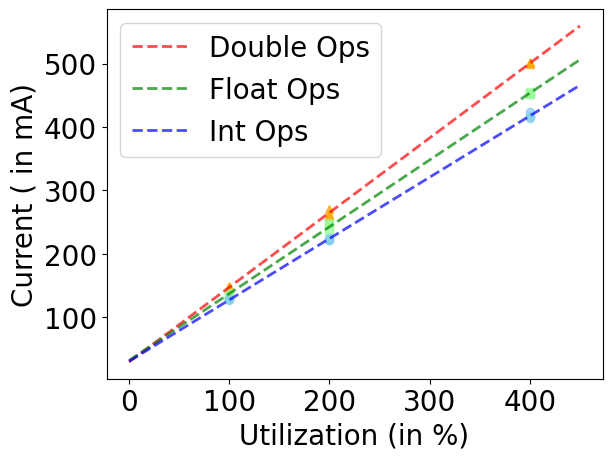
\includegraphics[width=\columnwidth]{figures/int_float_double.png}
    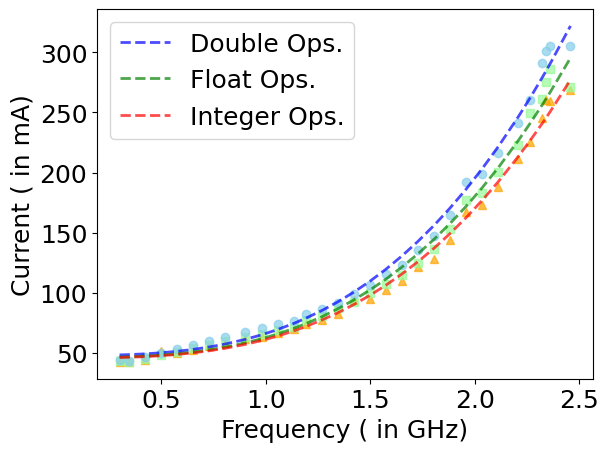
\includegraphics[width=\columnwidth]{figures/int_float_double_characteristics.png}
    \caption{CPU power for double, float and integer arithmetic operations.} % (for 1.8 GHz)}
    \label{fig:int_vs_float_vs_double}
    \end{subfigure}
    \caption{CPU power varies with app workload.}
    \label{fig:cpu_model_derivation}
    \vspace{-0.1in}
\end{figure}

\paragraph{Derived model}
Figure~\ref{fig:cpu_vs_mem} shows the derived CPU power model parameters
by plotting the total CPU power
as a function of the frequency.
% using the arithmetic-intensive and memory-intensive microbenchmarks. 
We observe that the CPU power draw for the two arithmetic-memory operation mix differ significantly,
by 38.7\% at the 300 MHz and 56.8\% at 2.45 GHz.
This suggests that the arithmetic-memory operation mix can send the CPU cores
to different power state variations draining different power.
In principle, this variation can be captured in the TPMD process by  
explicitly modeling memory as a separate phone component,
as in~\cite{carroll:2010,sesame:2011}, 
% gernot:2010 <- Koala: a platform for OS-level power management
using cache performance counter and free memory as the power triggers for memory draw. 
{
However, since the memory operation mix such as hardware counters is not collected by the mobile hardware 
or not reported by the Android OS on Android phones, it is much easier to lump memory power draw with CPU power draw as is commonly done in many recent work, including Android Battery Stats and Historian~\cite{androidbatterystats}. \comment{more example???}
}

Figure~\ref{fig:int_vs_float_vs_double} shows the derived CPU power model parameters for the integer only, 
float only, and double only arithmetic-intensive phases of the microbenchmark. 
We observe that the {CPU power} also differ, 
by 2.9\% at the 300 MHz and 13.5\% at 2.45 GHz.
This suggests that even the data type of arithmetic operations
can send the CPU cores into different power state variations.

\if 0
In summary, the above exercise of TPMD of CPU power shows the CPU power 
draw is very much app usage dependent and any fixed CPU model derived from
running a fixed microbenchmark is likely to have high estimation error when 
used in a particular app run. 
\fi


\if 0
\questionaj{This is not a very convincing argument. 1. For memory benchmark, is "CPU
power" = "CPU + memory" power? Or is the CPU power referenced in figure is true CPU 
power? If it is first, seeing higher "CPU power" is expected and not surprising.
2. Someone can argue that you could log memory triggers by instrumenting
compiler/libc/kernel,
why not just log?  Another paper didn't do it is not a strong reason. I think the 
argument we are trying to make is broader. That there are too many triggers that can 
affect a component power model. Because of which (a) micro-benchmark author may not 
know about all of them (b) building an exhaustive model could be expensive and not useful
as some model combinations may not even appear in real apps and (c) logging all 
triggers can be prohibitively expensive or not allowed. Because of this 
micro-benchmarks are hopelessly doomed.
If you agree,
we should also throw int-ops vs float-ops arithmetic, CPU temperature into the mix and use them to make the above three arguments.}
\fi



%%%%%%%%%%%%%%%%%%%%

% %% Flow of section
% % 2. Explain how memory operation effects CPU model
% {\bf Memory operation mix affects CPU power draw.}
% We performed the following experiments which showed that 
% the memory operation mix can significantly affect the CPU power draw at a fixed frequency.
% We wrote a microbenchmark program that runs arithmetic intensive operations for 7 seconds at 100\% utilization followed by a memory-intensive operation for 7 seconds at 100\% utilization.
% %% 2b. What we did
% We ran the microbenchmark 10 times for each of the big core frequencies on 1 core, while keeping all other cores offline.
% %% 2c. Explanation of results
% Figure~\ref{fig:cpu_vs_mem} shows that the average power consumed for the arithmetic-intensive microbenchmark 
% and for the memory-intensive microbenchmark differ significantly,
% by 40\% at the 300 MHz and by 57\% at 2.45 GHz.
% \begin{figure}
%     \centering
%     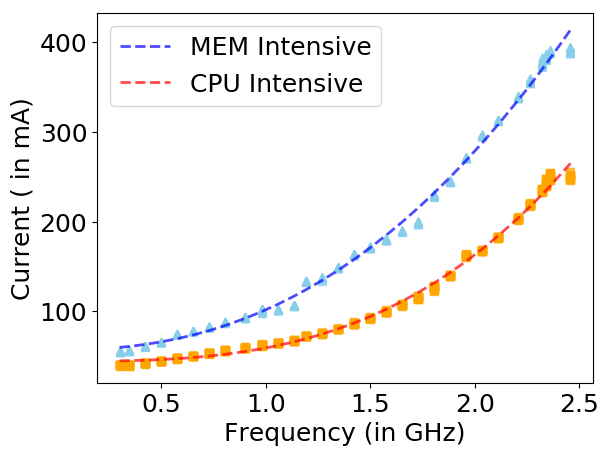
\includegraphics[width=0.75\columnwidth]{figures/cpu_mem_characteristics.png}
%     \caption{CPU power for compute-intensive and memory-intensive operations.}
%     \label{fig:cpu_vs_mem}
% \end{figure}





% In particular,
% we first developed a CPU-intensive benchmark that performs arithmetic computation in the busy loop and in % memory intensive benchmark we access different elements of a multidimensional array.
% We generated different models for CPU and memory intensive operations.
%
% {\bf CPU Model derivation\\}
%\subsection{GPU Power Model is App Dependent}
\label{subsec:gpu}

Next, we show the GPU power model can also be highly dependent on app usage. 
The GPU gives an example of a component that cannot be exercised alone and we show
how TPMD models the GPU power incrementally over the CPU model.

%%% Things discussed in this section
%% 1. Explain GPU is complex in modern smartphones
%% 2. Explain the GPU frequencies and power states in modern smartphones
%% 3. Explain complete GPU model
%% 4. What did we do
%% 5. Explain results and observation
%%   5a. Explain per scenario dependent modeling
%%   5b. Explain the reasons for the observation

%The GPU of modern phones can run at various frequencies and transition among various power states.
\paragraph{Parameters of the GPU power model}
In Moto Z3, the GPU can run at 7 different frequencies and has three power states,
Active, Slumber (offline), and Aware.
When the GPU is woken out of the Slumber state, it enters the Aware state for a brief duration.
% \comment{Similarly, Nexus 6 can run at 5 different frequencies and three power states; Active, Init and Nap. Init corresponds to Aware and Nap corresponds to Slumber of Moto Z3}
%{
% How does does it stay in Aware?
%This the initialization phase of the GPU.
% for a fixed duration? 535 uS on average ( with a 250 uS difference between 435 uS (min) and 635 us (max))
% }
The Active state has two sub states, Active-busy when the GPU is computing and Active-idle
when the GPU is idle. After staying in Active-idle for a threshold interval, the GPU enters the Slumber state.
Since the GPU never enters the Slumber or Aware state when an app is running, 
the parameters of the GPU model include only the GPU power draw in Active-busy and Active-idle in each frequency, $p^g_{busy}(g_k), p^g_{idle}(g_k)$, as listed in Table~\ref{tab:parameters}.
We abbreviate Active-busy and Active-idle states simply
as GPU Busy and Idle states in the rest of the paper.

\if 0
Accordingly, we model the GPU power draw as follows:
\begin{equation}
    Power_{GPU} = \sum_{j}\sum_{i} u_{ij}*p_{ij}
    \end{equation}
where $p_{ij}$ is the power parameter for the $i^{th}$ GPU frequency for the $j^{th}$ power state (Active-busy, Active-idle, Slumber, Aware) and $u_{ij}$ is the corresponding utilization in that frequency and power state.
\fi

\paragraph{TPMD methodology}
% Similar to CPU, the GPU of modern smartphones have also vastly developed.
Initially, we tried to use a GPU benchmark, 3DMark~\cite{3DMark}, to drive the GPU usage into Busy and Idle states under each frequency.
However, we found that the GPU benchmark renders very different consecutive frames which
result in rapidly fluctuating GPU utilizations and power monitor readings.
This makes aligning the power monitor readings with the GPU Busy periods difficult
which is needed to extract the GPU Busy state power at each frequency.
%
% In power trace it was difficult to identify busy and idle traces for GPU benchmarks.This is because utilization is not constant as it continually generates new frames and can’t be paused.
% In apps the GPU utilization is constant because when no input is given to  the game app it generates the same frame again and again.
%
% we can only generate average GPU power coefficients for GPU busy and idle states.
% Average GPU coefficient depends on GPU utilization i.e  the time GPU is busy to total GPU running time.
%Average GPU power coefficients so derived is fixed and can not cater to two apps which may have different GPU utilization.
In contrast, we observe that real apps tend to render very similar consecutive frames in a short period of time which result relatively stable GPU utilization and stable GPU power draw, 
making it much easier to extract the power monitor reading corresponding to a given GPU utilization
(see Figure~\ref{fig:power_trace_candycrushturorial} later). 
%  the rendering task often finishes in less than the 16.7ms per-frame interval and hence the GPU will go through busy and idle states in every 16.7ms interval, making it much easier to manually identity both states. 
% \questionaj{Why do we have to identify manually? Triggers are not available in atrace?
% Due to both drift and scaling their is vast alignment problem in aligning each 16.7 ms interval.
% Alignment problem prevent us from directly using triggers from the event trace.}
Based on this observation, we directly used selected apps that use 
only the CPU and GPU to derive the GPU power models. 
In particular, we derive the CPU model first using the integer-arithmetic microbenchmark\footnote{We found using the CPU model derived using memory-intensive microbenchmark
resulted in negative GPU coefficients.}
and then use the difference 
between the measured phone power and model-estimated CPU power as the ground-truth for the GPU power draw
in GPU power model derivation.


% 5. Explain results and observation

\begin{table*}[tp]
{\footnotesize
    \centering
    \caption{Moto Z3 GPU power model (Busy and Idle power per frequency) with the CPU fixed at 1.056 GHz.}
    \vspace{-0.1in}
    \begin{tabular}{|p{11.5mm}|p{22mm}|c|c|c|c|c|c|c|c|c|c|c|c|c|c|}
    \hline
    App & Scenario & \multicolumn{14}{c|}{GPU Frequency} \\
    \cline{3-16}
     &  & \multicolumn{2}{c|}{257 MHz} & \multicolumn{2}{c|}{342 MHz} & \multicolumn{2}{c|}{414 MHz} & \multicolumn{2}{c|}{515 MHz} & \multicolumn{2}{c|}{596 MHz} & \multicolumn{2}{c|}{670 MHz} & \multicolumn{2}{c|}{710 MHz} \\
     \cline{3-16}
     & & Busy & Idle & Busy & Idle & Busy & Idle & Busy & Idle & Busy & Idle & Busy & Idle & Busy & Idle \\
    \hline
       \multirow{3}{11mm}{Boat Racing}  & Intro & 208.5 & 134.7 & 253.7 & 67.25 & 283.2 & 149.9 & 423.6 & 124.5 & 581.6 & 79.85 & 633.2 & 162.2 & 703.2 & 184.2 \\
       \cline{2-16}
        & Still & 232.3 & 145.5 & 358.0 & 57.00 & 402.8 & 153.0 & 573.9 & 92.17 & 576.3 & 150.0 & 813.9 & 145.0 & 866.3 & 205.9 \\
         
         & GPU engy. error (\%) & 232.3 & 145.5 & 358.0 & 57.00 & 402.8 & 153.0 & 573.9 & 92.17 & 576.3 & 150.0 & 813.9 & 145.0 & 866.3 & 205.9 \\
         
         \hline
        \multirow{2}{11mm}{Bricks Breaker}  & Intro & 140.7 & 70.33 & 158.3 & 69.32 & 204.3 & 109.9 & 166.8 & 134.4 & 130.0 & 141.3 & 115.5 & 172.9 & 133.2 & 191.4 \\
       \cline{2-16}
         & Still & 180.8 & 72.69 & 185.5 & 72.63 & 177.7 & 113.0 & 243.6 & 112.8 & 271.3 & 115.6 & 375.7 & 138.1 & 441.2 & 154.7 \\
         \hline
        \multirow{2}{13mm}{Candy Crush Saga}  & Into & 228.0 & 83.88 & 262.5 & 83.97 & 344.4 & 112.7 & 523.1 & 123.3 & 620.7 & 120.0 & 792.6 & 146.2 & 900.4 & 167.2 \\
        \cline{2-16}
         & Tutorial & 226.3 & 92.85 & 228.4 & 89.50 & 330.6 & 117.7 & 445.2 & 134.5 & 519.6 & 137.5 & 660.2 & 160.7 & 855.3 & 171.6 \\
         \hline
    \end{tabular}
    \label{tab:gpumodel_motoz3}
    \vspace{-0.1in}
    }
\end{table*}

% Comparison Table for GPU model with other scenarios Here

We repeated the GPU model derivation for three
popular games apps, Boat Racing, Candy Crush Saga and Bricks breaker.
each running two scenarios, as listed in Table~\ref{tab:app_scenario_description}.
To minimize the variance of CPU power draw, we fixed the CPU frequency at 1.056 GHz,
and ran each app scenario under each GPU frequency for a duration of 60 seconds.

\paragraph{Derived model}
Table~\ref{tab:gpumodel_motoz3} shows the derived GPU power models for varying GPU frequencies for Moto Z3 and Table~\ref{tab:gpumodel_nexus6} for Nexus 6.
%% 5a. Explain per scenario dependent modeling
We make two observations.
(1) The GPU power parameters for the same frequency differ with {\it different apps}; at 710 MHz, the GPU Busy power draw for Boat Racing is 10.6\% lower than for Candy Crush Saga on Moto Z3.
(2) The GPU parameters for the same frequency even differ for {\it different scenarios} 
of the same app; for Boat Racing, the GPU Busy power draw
for the Intro scenario is 10.2\% and 29.7\% lower than for the Still scenario
at 257 MHz and 414 MHz, respectively.

To show the importance of app-specific power modeling, we calculated the error
in estimating the total GPU energy drain in the second scenario of each app 
if using the GPU model derived using the first scenario of each app.
Table~\ref{tab:gpumodel_motoz3} shows that the error ranges between 
??\%--??\%, ??\%--??\%, and ??\%--??\% for the second scenarios of the three apps.


%% 5b. Explain the reasons for the observation
The above dependence of the GPU power draw on app usage can be attributed  to two main reasons.
First, the GPU has a large number of mini-cores, but the utilization metric available to the OS only captures the temporal utilization but not the spatial utilization, \ie the percentage of mini-cores that were active.
Different spatial utilization may drive the GPU into different power state variations that have the same temporal utilization but different power draw.

Second, rendering different frames in different scenarios of the same app or different apps may result in different memory operation mix, and hence using a single CPU model in estimating the CPU power draw portion to be subtracted from the total phone power 
may result in errors in the GPU power draw  estimation, as we see in \S\ref{sec:primer_cpu}. 
Such error propagation happens in TPMD which models one component at a time
and often relies on the models for prior components to estimate the "ground truth" in modeling  the next component. 


% \subsection{GPU Power Model is App Dependent}
% \label{subsec:gpu}

\paragraph{Parameters of the CPU and GPU power models}
Moto Z3~\cite{motoz3} is a representative modern smartphone
that uses the big.LITTLE CPU architecture~\cite{biglittlearch} to
provide energy efficiency in supporting diverse workloads.
Particularly, in Moto Z3, the LITTLE cores can operate in 22 different frequencies 
and big cores can operate in 31 different frequencies.
%  The cores are switched to higher frequencies when higher performance is required.
At runtime, the OS scheduler along with the CPU governor performs power state transition and core frequency scaling to optimize the CPU energy draw as the workload varies.
Thus the parameters of the CPU power model include
the base power consumed $p_{base}$ when the cores are idle and
the non-base core $i$ power running at frequency $f_k$, $p^c_i(f_k)$, as listed in Table~\ref{tab:parameters}.
The total CPU power can be modeled~\cite{multicoremodel:2015} as:
{
\begin{equation}
    P_{CPU} = p^c_{base} + \sum_{i} p^c_i(f_k)
\end{equation}

}

%\paragraph{Parameters of the GPU power model}
In Moto Z3, the GPU can run at 7 different frequencies and has three power states,
Active, Slumber (offline), and Aware.
% When the GPU is woken out of the Slumber state, it enters the Aware state for a brief duration.
% The Active state has two sub states, Active-busy when the GPU is computing and Active-idle
% when the GPU is idle. After staying in Active-idle for a threshold interval, the GPU enters the Slumber state.
Since the GPU never enters the Slumber or Aware state when an app is running, 
the parameters of the GPU model include only the GPU power draw in Active-busy and Active-idle states in each frequency, $p^g_{busy}(g_k), p^g_{idle}(g_k)$, as listed in Table~\ref{tab:parameters}.
We abbreviate Active-busy and Active-idle states simply
as GPU Busy and Idle states in the rest of the paper.

\if 0
Accordingly, we model the GPU power draw as follows:
\begin{equation}
    Power_{GPU} = \sum_{j}\sum_{i} u_{ij}*p_{ij}
    \end{equation}
where $p_{ij}$ is the power parameter for the $i^{th}$ GPU frequency for the $j^{th}$ power state (Active-busy, Active-idle, Slumber, Aware) and $u_{ij}$ is the corresponding utilization in that frequency and power state.
\fi

\paragraph{TPMD methodology}
We first derived CPU power models using microbenchmarks that perform arithmetic and memory operations for 7 seconds each 
with 100\% utilization.
We ran the microbenchmark while fixing the big core cluster at each of the 31 frequencies for both Pixel 2 and Moto Z3 and at each of the 17 frequencies for Pixel 4, 
on 1 core and 2 cores.
% When using 1 core, 2 cores and 4 cores, the remaining cores are offline.
We measure the base CPU power as the phone power draw when all cores are idle.
We manually align the power monitor readings for each of the 7-second interval 
and derive the non-base per-core power for each frequency by 
subtracting the base power from the measured total phone power.
{For the phones, we found that the per-core power $p_i(f_k)$ remains the same for different cores.}

% Similar to CPU, the GPU of modern smartphones have also vastly developed.
% Initially, we tried to use a GPU benchmark, 3DMark~\cite{3DMark}, to drive the GPU usage into Busy and Idle states under each frequency.
\begin{sloppy}
For the GPU, we found that GPU benchmarks, \eg 3DMark~\cite{3DMark}, typically render quite different consecutive frames which
result in rapidly fluctuating GPU utilizations and power monitor readings,
making the alignment difficult. 
\end{sloppy}
%
% This makes aligning the power monitor readings with the GPU Busy periods difficult
% which is needed to extract the GPU Busy state power at each frequency.
%
In contrast, we observe that real apps tend to render very similar consecutive frames in a short period of time which result relatively stable GPU utilization and stable total power draw, 
making it much easier to extract the power monitor reading corresponding to a given GPU utilization
(see Figure~\ref{fig:power_trace_candycrushturorial} later). 
%  the rendering task often finishes in less than the 16.7ms per-frame interval and hence the GPU will go through busy and idle states in every 16.7ms interval, making it much easier to manually identity both states. 
% \questionaj{Why do we have to identify manually? Triggers are not available in atrace?
% Due to both drift and scaling their is vast alignment problem in aligning each 16.7 ms interval.
% Alignment problem prevent us from directly using triggers from the event trace.}
Thus, we directly used selected apps that use only the CPU and GPU to derive the GPU power models. 
In particular, we 
derive the CPU model by first using the 
% integer-arithmetic 
CPU arithmetic microbenchmark\footnote{We found using the CPU model derived using memory-intensive microbenchmark resulted in negative GPU coefficients.} 
and then 
using the difference between the measured phone power and model-estimated CPU power when running an app  to determine the ground-truth for the GPU power draw and GPU power model derivation.


% 5. Explain results and observation

\begin{figure*}[tp]
    \centering
     \begin{subfigure}[b]{0.32\textwidth}
         \centering
         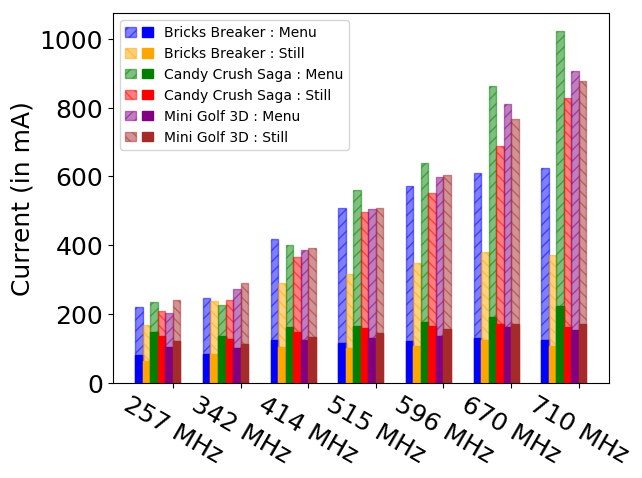
\includegraphics[width=\textwidth]{figures/002_Pixel2_gpu_model.png}
         \caption{Pixel 2}
         \label{fig:number_parameters_vs_duration_100s_0}
     \end{subfigure}
    \begin{subfigure}[b]{0.32\textwidth}
         \centering
         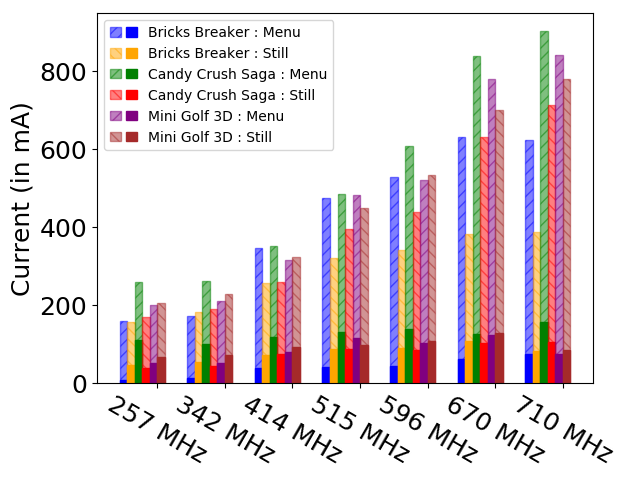
\includegraphics[width=\textwidth]{figures/003_MotoZ3_gpu_model.png}
         \caption{Moto Z3}
         \label{fig:number_parameters_vs_duration_100s_100}
     \end{subfigure}
    \begin{subfigure}[b]{0.32\textwidth}
         \centering
         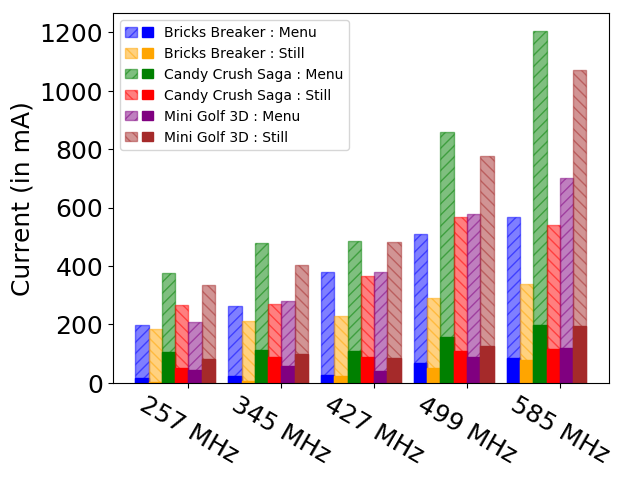
\includegraphics[width=\textwidth]{figures/004_Pixel4_gpu_model.png}
         \caption{Pixel 4}
         \label{fig:number_parameters_vs_duration_100s_200}
     \end{subfigure}
     \hfill
    \caption{GPU power model (Busy power in hatched and Idle power in solid) with the CPU fixed for the 3 phones.}
    \label{fig:gpu_model}
    \vspace{-0.1in}
\end{figure*}

\begin{table*}[]
    \caption{Energy estimation error (\%) for app scenarios 
    using the GPU model derived for each scenario with CPU and GPU fixed frequencies for the 3 phones. (B: Bricks Breaker, C: Candy Crush Saga and M: Mini Golf 3D)}
    \centering
     \begin{subfigure}[b]{0.32\textwidth}
        \centering
    	{ \scriptsize
    	\begin{tabular}{ | l | c | c | c | c | c | c | }
    		\hline
    		     & \multicolumn{6}{ c|}{Error for each App Scenarios (in \%)}\\
    		\cline{2-7}
                    Model & \rot{B. Menu} & \rot{B. Still} & \rot{C. Menu} & \rot{C. Still} & \rot{M. Menu} & \rot{M. Still}  \\
    		\hline
                B. Menu              & 8.9 & 13 & 20 & 16 & 11 & 14 \\
                B. Still             & 15 & 11 & 31 & 25 & 17 & 26 \\
                C. Menu              & 16 & 24 & 11 & 11 & 13 & 11 \\
                C. Still             & 16 & 19 & 14 & 12 & 12 & 14 \\
                M. Menu              & 9.9 & 14 & 14 & 11 & 8.1 & 11 \\
                M. Still             & 12 & 21 & 9.7 & 10 & 11 & 8.6 \\
    		\hline
    	\end{tabular}
    	}
	\caption{Pixel 2}
    \end{subfigure}
     \begin{subfigure}[b]{0.32\textwidth}
        \centering
    	{ \scriptsize
    	\begin{tabular}{ | l | c | c | c | c | c | c | }
    		\hline
    		     & \multicolumn{6}{ c|}{Error for each App Scenarios (in \%)}\\
    		\cline{2-7}
                    Model & \rot{B. Menu} & \rot{B. Still} & \rot{C. Menu} & \rot{C. Still} & \rot{M. Menu} & \rot{M. Still}  \\
    		\hline
                B. Menu              & 16 & 18 & 44 & 18 & 22 & 25 \\
                B. Still             & 18 & 15 & 36 & 15 & 17 & 17 \\
                C. Menu              & 30 & 24 & 16 & 23 & 18 & 16 \\
                C. Still             & 12 & 12 & 31 & 11 & 15 & 17 \\
                M. Menu              & 18 & 16 & 23 & 15 & 14 & 15 \\
                M. Still             & 20 & 15 & 20 & 14 & 12 & 13 \\
    		\hline
    	\end{tabular}
    	}
	\caption{Pixel 2}
    \end{subfigure}
         \begin{subfigure}[b]{0.32\textwidth}
        \centering
    	{ \scriptsize
    	\begin{tabular}{ | l | c | c | c | c | c | c | }
    		\hline
    		     & \multicolumn{6}{ c|}{Error for each App Scenarios (in \%)}\\
    		\cline{2-7}
                    Model & \rot{B. Menu} & \rot{B. Still} & \rot{C. Menu} & \rot{C. Still} & \rot{M. Menu} & \rot{M. Still}  \\
    		\hline
                B. Menu              & 15 & 15 & 44 & 19 & 15 & 34 \\
                B. Still             & 15 & 15 & 50 & 23 & 17 & 40 \\
                C. Menu              & 30 & 33 & 12 & 20 & 25 & 13 \\
                C. Still             & 18 & 20 & 25 & 15 & 16 & 19 \\
                M. Menu              & 15 & 16 & 34 & 17 & 14 & 26 \\
                M. Still             & 25 & 28 & 13 & 15 & 21 & 12 \\
    		\hline
    	\end{tabular}
    	}
	\caption{Pixel 2}
    \end{subfigure}
    \label{fig:gpu_model_error}
    \vspace{-0.1in}
\end{table*}
% Comparison Table for GPU model with other scenarios Here

We repeated the GPU model derivation for three
popular games apps, Bricks Breaker, Candy Crush Saga and Mini Golf 3D,
each running two scenarios, as listed in Table~\ref{tab:app_scenario_description}.
To minimize the variance of CPU power draw, we fixed the CPU frequency at 1.42 GHz for both Pixel 2,Moto Z3 and 1.61 GHz for Pixel 4,
and ran each of the app scenario under each GPU frequency for a duration of 30 seconds.

\paragraph{Derived model}
Our CPU modeling results (details omitted) show that
the CPU power draw for the arithmetic-intensive and memory-intensive
operations of the microbenchmark differ significantly,
by 38.7\% at the 300 MHz and 56.8\% at 2.45 GHz for Moto Z3.
This suggests that the arithmetic-memory operation mix can send the CPU cores
to different power state variations draining different power.
Figure~\ref{fig:gpu_model}(a)-(c) shows the derived GPU power models for varying GPU frequencies for the 3 phones. The full bars represent the busy current whereas the solid bars are the idle current.
% and Table~\ref{tab:gpumodel_nexus6} for Nexus 6.
%% 5a. Explain per scenario dependent modeling
From our findings we make two observations.
(1) The GPU power parameters for the same frequency differ with {\it different apps}; on Moto Z3 at 710 MHz, the GPU Busy power draw for Bricks Breaker Still is 57.2\% lower than for Candy Crush Saga Menu.
(2) The GPU power parameters for the same frequency even differ for {\it different scenarios} 
of the same app; for Bricks Breaker, the GPU Busy power draw
for the Still scenario is 32.3\% and 35.5\% lower than for the Menu scenario  at 515 MHz and 596 MHz respectively for Moto Z3.
Other phones also show simlar findings.

%% 5b. Explain the reasons for the observation
The above dependence of the GPU power draw on app usage can be attributed  to two main reasons.
First, the GPU has a large number of mini-cores, but the utilization metric available to the OS only captures the temporal utilization and not the spatial utilization, \ie the percentage of mini-cores those were active.
Different spatial utilization may drive the GPU into different power state variations that have the same temporal utilization but different power draw.


Second, using a single CPU model in estimating the CPU power draw which is to be subtracted from the total phone power may result in errors in the GPU power draw  estimation,
 as rendering different frames for different app scenarios (of the same or different apps) may result in different CPU usage, \eg due to different mix of arithmetic and memory operations and hence CPU power draw.
Such error propagation happens in TPMD which models one component at a time
and often relies on the models of a  prior component to estimate the "ground truth" in modeling  the next component. 

\paragraph{Cross validation}
To confirm that the GPU models derived per app scenario captures models dependence on the app usage also, we perform  a cross validation by applying
the GPU model derived from each of the six app scenarios shown in Figure~\ref{fig:gpu_model}(a)-(c)
and estimate the total energy of all app scenarios (including self). As shown in 
Figure~\ref{fig:gpu_model_error}(a)-(c) for the case where GPU frequency at 257 MHz  and CPU frequency 
fixed at 1.42 GHz for Pixel 2 and Moto Z3 and 1.61 GHz fixed for Pixel 4,
we observe that the error is the lowest when the GPU model specific to an app scenario is applied
to itself (same app scenario) i.e. the diagonal in the figure has the lowest error.
% \comment{
% We observe that the lowest error for a scenario is
% due to GPU model derived from same scenario (fitting error), whereas for
% all other scenario GPU models the error can be as much as 2$times$ higher.
% For the higher GPU frequencies, like 710 MHz the difference in the can increase up to about 10 times.
% }


\if 0
we calculated the error
in estimating the total GPU energy drain in the second scenario of each app 
if using the GPU model derived using the first scenario of each app.
The rows labelled "GPU energy error" in Table~\ref{tab:gpumodel_motoz3} shows that the error ranges between ??\%--??\%, ??\%--??\%, and ??\%--??\% for the second scenarios of the three apps.
\fi







\paragraph{Summary}
The above exercise of applying TPMD to derive the GPU models for 6 app scenarios 
have two important implications.
(1) The GPU power draw is very much dependent on app usage ; different app usage can lead to  variations of the same power state, drawing different amount of 
power. Hence {\it any fixed GPU model derived from
running a particular microbenchmark or app is likely to have high estimation error when 
it is applied for a different app run.} This motivates the need for SPMD which is inherently app usage specific. 
(2) Since different scenarios of the same app can drive components into different
power state variations, {\it the equations from different scenarios of the same app run should not be 
grouped into the same system of equations to be fed into the solver in SPMD,}
as this defeats the app usage specificity nature of SPMD. 


\section{Self Power Modeling Methodology}
\label{sec:method}

In this section, we describe the basic self power modeling methodology,
we added the constraints to the basic solver in an effort to help the solver to output meaningful model parameters, and for the usabiity of Android phones power sensor readings.  

% as depicted in Figure~\ref{fig:equations}.
\if 0
\begin{figure}[tp]
    \centering
    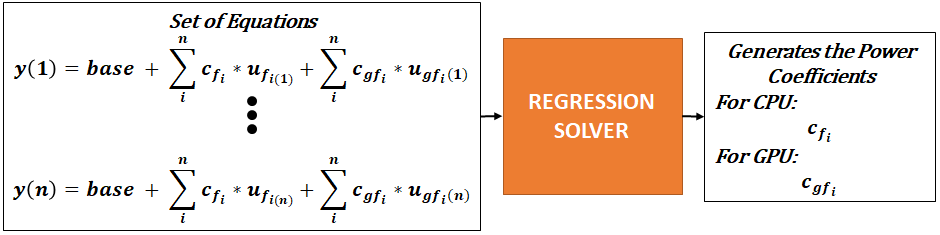
\includegraphics[width=0.95\columnwidth]{figures/design_2.png}
    \vspace{-0.1in}
    \caption{SPMD via solving a system of linear equations.}
    \label{fig:equations}
    \vspace{-0.1in}
\end{figure}
\fi

\begin{table}[t]
{\footnotesize
    \centering
    \caption{Power state, utilization, and energy collected during online app run.}
    \vspace{-0.1in}
   % \begin{tabular}{|p{32mm}|p{10mm}|p{23mm}|}
    \begin{tabular}{|l|P{11mm}|c|}
    \hline
          &  Symbol & Collection method \\
         \hline
         \multicolumn{1}{|l|}{\textbf{Power State}} &  &   \\
         CPU Frequency      & $f_{k}$                               & cpu\_frequency \\
         GPU Frequency      & $g_{k}$                               & kgsl\_pwrlevel \\
         GPU State          & $s_j$                                 & kgsl\_pwr\_set\_state \\
         \hline
          \multicolumn{1}{|l|}{\textbf{Utilization}} &   &  \\
         
         \multicolumn{1}{|l|}{CPU Util. in freq. $f_k$}               & $u^c(f_{k})$        & cpu\_idle \\
         \multicolumn{1}{|l|}{GPU Util. in freq. $g_k$, state $s_j$}  & $u^g(g_k,s_j)$      & kgsl\_pwrstats \\
         \hline
         \multicolumn{1}{|l|}{Energy drain}     & $y$                                &
         \multicolumn{1}{p{30mm}|}{/sys/class/power\_supply /charge\_counter} \\
         \hline
    \end{tabular}
    \label{tab:triggers}
    \vspace{-0.1in}
}
\end{table}


% \comment{Placeholder: We may or may not need to discuss power triggers for other phone components
% to make this section general.}

\subsection{Basic SPMD Process}
\label{subsec:generic}

As discussed in \S\ref{subsec:spmd}, SPMD consists of two basic steps: 
online data collection for setting up a system of equations and 
offline model derivation by solving the system of equations.

\paragraph{Online data collection}
Since SPMD is "in-situ", collecting data  is needed to set up the equations  while the app is running. 
% As discussed in \S\ref{sec:primer}, in modern phones, the CPU and GPU power draw are 
% functions of the operating frequency and the power state (for GPU). Therefore,
% for power triggers, we need to collect the duration each component spends in every 
% combination of frequency and power-state during the app run, as listed in Table~\ref{tab:triggers}.
%
Table~\ref{tab:triggers} lists the data that need to be collected and how they are collected. 
The data include the power states and utilization in each state , for each component used by the app  , for each time interval corresponding to an equation as well as  the whole-phone energy drain.

We use the Linux event trace~\cite{eventtrace} to collect the power state and utilization. 
To collect whole-phone energy draw per interval, we can use either the built-in power sensor energy counter which became available since Android \comment{7}, or an external power monitor such as Monsoon~\cite{monsoonpowermonitor}.

\cut{ Ideally, reading from the built-in power sensor is preferred, since it does not require wiring the phone battery and potentially allows SPMD to be performed on any phones, including users' phones "in the wild". However, as we will see in the next section, built-in power sensor readings have such high error that makes them impractical to use in SPMD. 
}

\if 0
\begin{figure}[tp]
{\small
    \centering
    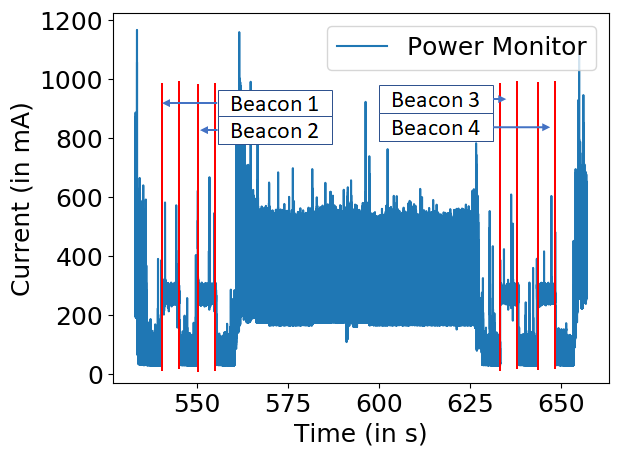
\includegraphics[width=0.80\columnwidth]{figures/beacons_3.png}
    \vspace{-0.1in}
    \caption{Beacons to align power monitor with phone clock.}
    \label{fig:align_beacon}
    \vspace{-0.1in}
}
\end{figure}
\fi

%%%%%%%%%%%%%%%
\paragraph{Offline model derivation} 
%
In offline processing, \eg when the app completes it running and data for model derivation is available, SPMD sets up a system of linear equations with the phone component power parameters as unknowns.
In general, the trace duration is cut into $K$ equal intervals of $T$ seconds each, and one equation is created for interval $t$ as follows:
\begin{equation}
y_t = p^{c}_{base}+ \sum_i\sum_k{u^c_t(f_k)*p_i^{c}(f_{k})} + 
            \sum_{j}\sum_{k} u^g_t(g_k,s_j)*p^{g}(g_k, s_j)
\end{equation}
where the double summation for the CPU is over all the CPU cores and frequencies,
the double summation for the GPU is over all the GPU frequencies and GPU states,
$u^c_t(f_k)$ and $u^g_t(g_k,s_j)$ are the CPU and GPU utilization for the corresponding power states
in time interval $k$,
and the left-hand-side (LHS) $y_t$ is the total phone energy drain in time interval $t$.
% where model parameter $p^c(f_{i})$ is the CPU power draw for frequency $f_i$,  
% model parameter $p^g_{ij}$ is the GPU power draw at frequency $f_i$ and power state $j$, the utilization coefficients $_{f_{i}}(k)$ and $u_{ij}(k)$ equal the total utilization (in seconds) of CPU and GPU in the corresponding frequencies and power states in the $k$th trace interval, and $y(k)$ denotes the total phone energy drain during interval $k$ from integrating power sensor or power monitor readings.
\cut{ 
Clearly, in a given app run, the CPU and GPU may not go through all possible frequencies and power states, and hence not all power parameters may show up in the equations. SPMD will only derive those power model
parameters actually encountered in the app run. This is not an issue with SPMD as only those parameters will be needed for the power model applications such as energy profiling or energy debugging. 
}

Since there can be more equations than the number of unknowns, 
the sytem of equations can be solved using a regression-based solver to generate the power parameters.
In this paper, we use the python curve\_fit() function which uses a non-linear least square fitting as our regression solver~\cite{curvefit}.

SPMD via solving a system of equations using a regression solver is conceptually simple. 
However in practice, the single biggest challenge is whether the system of equations 
has got enough diversity so that the regression solver
can generate meaningful solutions to the system of euations , \ie power model parameters. 

\if 0
\subsection{SPMD Challenges}
\label{subsec:challenges}

SPMD via solving a system of equations using a regression solver is conceptually simple. 
In practice, the single biggest challenge is whether the system of equations 
has enough diversity so that the regression solver
can generate meaningful solutions to the system, \ie power model parameters. 
The answer is not obvious for at least two reasons. 

{\bf Condition 1: Usage coefficients lack diversity.}
First, \S\ref{sec:primer} has concluded that
we need to set up a system of equations for each app scenario as different scenarios
even of the same app can have different component usage. However, 
one can imagine that the app behavior for the same app scenario may be highly repetitive and hence
the resulting equations, either the usage terms on one side or the energy drain on the other side,
 may look similar or only differ slightly, resulting on low rank of the equations. 

{\bf Condition 2:s Noisy energy measurement.}
The energy measurement can contain noise and if the difference among the true energy values for different equations is small, the noise level may dominate the energy variations of the different equations. This can result in the regression solver trying to minimize the fitting error from noisy energy measurement as opposed to fitting the true energy difference.  

Our verification study centers around addressing this challenge, by systematically exploring different ways of setting the system of equations to try to increase the diversity.

Before presenting our verification study, we discuss two refinements we added
to the basic SPMD methodology.


\fi

\subsection{Adding Constraints to the Solver}
\label{subsec:constraint}

\if 0 
As we will see in \S\ref{sec:modelling_macro}, 
when the system of liner equations suffers the two conditions above, the regression solver may output different solutions that all minimize the fitting error, which may violate basic properties of the power model parameter values. To overcome this, in addition to the basic unconstrained solver, 
\fi 
We experimented with adopting two ways for constraining the solutions generated by the regression solver based on simple domain knowledge, as shown in Table~\ref{tab:constrained}.

\begin{table}[tp]
%\questionaj{These constraints must also constrain GPU busy and idle.}
{\small
    \centering
    \caption{Constraints added to the regression solver.}
    \vspace{-0.1in}
    \begin{tabular}{|p{25mm}|p{52mm}|}
    \hline
         Constrainted SPMD  & \multicolumn{1}{c|}{Description} \\
         \hline
         Unconstrained      & No constraints are applied. \\
         Constrained        & Model parameters should not decrease with increasing frequencies. GPU idle power is less than Budy power. \\
         Freq-constrained   & CPU model parameters are modeled as a polynomial of frequency. \\
         \hline
    \end{tabular}
    \label{tab:constrained}
    \vspace{-0.1in}
}
\end{table}


\paragraph{Constraint 1: positivity and monotonicity}
Without any constraint, we found the regression solver can output CPU/GPU power values those are negative or 
decreasing while the frequency increases.
To prevent the solver from outputing such solutions, we add three constraints to the regression solver: 
(1) all model parameters should be positive;
(2) the model parameters with increasing frequencies for each component should be non-decreasing;
(3) the GPU Idle power should be lower than the GPU Busy power. 
We denote this version of SPMD as "Constrained SPMD" in Table~\ref{tab:constrained}.


\paragraph{Constraint 2: modeling CPU power as a function of frequency}
We found even with Constraint 1, the 
CPU power parameters output by the solver often does not change with varying frequencies. 
To make the CPU model parameters output more consistent with the reality, 
we exploited another domain knowledge about the CPU power draw,
that the power draw increases as per a low-order polynomial of the operating frequency~\cite{armdvfs,rizvandi2011some}.
% Since the specific polynomial function may vary for different phones, \eg early phones only performed % frequency scaling (FS) while newer phones perform dynamic voltage and frequency scaling (DVFS), we first used a simple CPU benchmark to find the order of the polynomial for each phone used in our experiments. 
%
\if 0
\begin{figure}[tp]
    \centering
%    \vspace{-0.1in}
    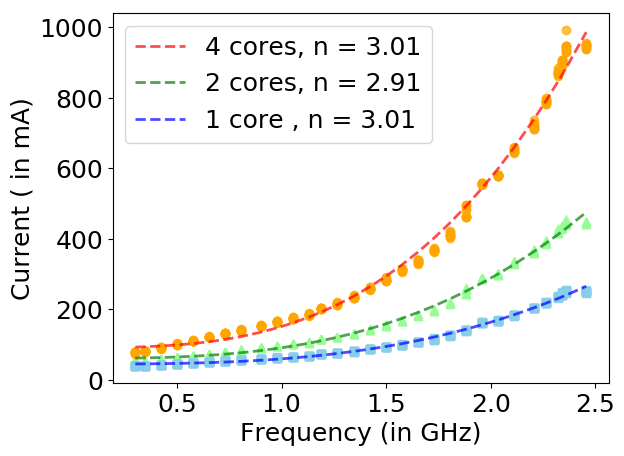
\includegraphics[width=0.80\columnwidth]{figures/cpu_characteristics.png}
    \caption{Moto Z3 big core CPU power draw grows with frequency 
    when running the arithmetic-intensive benchmark.}
    \label{fig:cpu_characteristic}
    \vspace{-0.1in}
\end{figure}
\fi
%
\cut{ We ran a microbenchmark that performs arithmetic-intensive or memory-intensive operations for 7 seconds
on 1, 2 and 4 big cores, for each big core frequency, and fit the measured phone power 
with a polynomial function in frequency.
%\begin{equation}
%     P_{CPU} = p^c_{base}+ \sum_i p^c_i({f_k}) = p_{base}+\sum_i  a*f_k^{n}
% \end{equation}
% Figure~\ref{fig:cpu_characteristic} shows the measured power draw and curve fitting on Moto Z3.
}
Our CPU microbenchmark results show show that 
% the fitted exponent $n$ for 1, 2 and 4 cores are 3.01, 2.97 and 3.01, respectively.
the per core power of Moto Z3 grows as the third-power of the CPU frequency.
Thus we replace all the CPU power parameters with third-power of the CPU frequency in the SPMD model equations.
%model the Moto Z3 big core power as a third-order polynomial of the CPU frequency in the model equations of SPMD.
%
Doing so has two benefits: (1) it reduces the number of CPU power parameters from $K$ - the number of CPU frequencies - to 2, $p_{base}$ and coefficient $a$, which reduces the number of equations needed for the solver; (2) it puts constraints for the CPU power  to be not only  monotonic, but consistent with physics.


\subsection{Can Power Sensor Readings be Used?}
\label{subsec:modelling_sensor}

Since using the built-in power sensor readings would allow SPMD to be performed on any phone in the wild,
we assess the feasibility of using the power sensors in modern smartphones for developing SPMD,
by measuring the accuracy of their the energy counter readings.

%{\bf Methodology }
%% 2. Explanation of equation generation
% Since in principle, the energy counter gives more accurate energy estimation for an equation interval than averaging all the instantaneous power readings in the interval multiplied by the interval duration,
% we use energy counter readings to generate the LHD of each model equation.
\begin{sloppy}
% The Android versions on both phones exports APIs for power sensor readings with
Android 7.0 and later provide 
interfaces to the built-in power sensor through sysfs~\cite{linuxsysfs} with
a finite sampling resolution, 1.4s on Pixel 2 and Moto Z3 and 380 ms on Pixel 4.
\comment{The power sensor readings have two formats}: instantaneous power draw 
({\small /sys/\-class/\-power\_supply/\-battery/\-current\_now}) and
energy counter ({\small /sys/\-class/\-power\_supply/\-battery/\-charge\_counter})
which reports the total energy in the previous sampling interval.
\end{sloppy}

\begin{figure}[tp]
    \centering
\if 0
\begin{subfigure}[b]{0.50\textwidth}
         \centering
         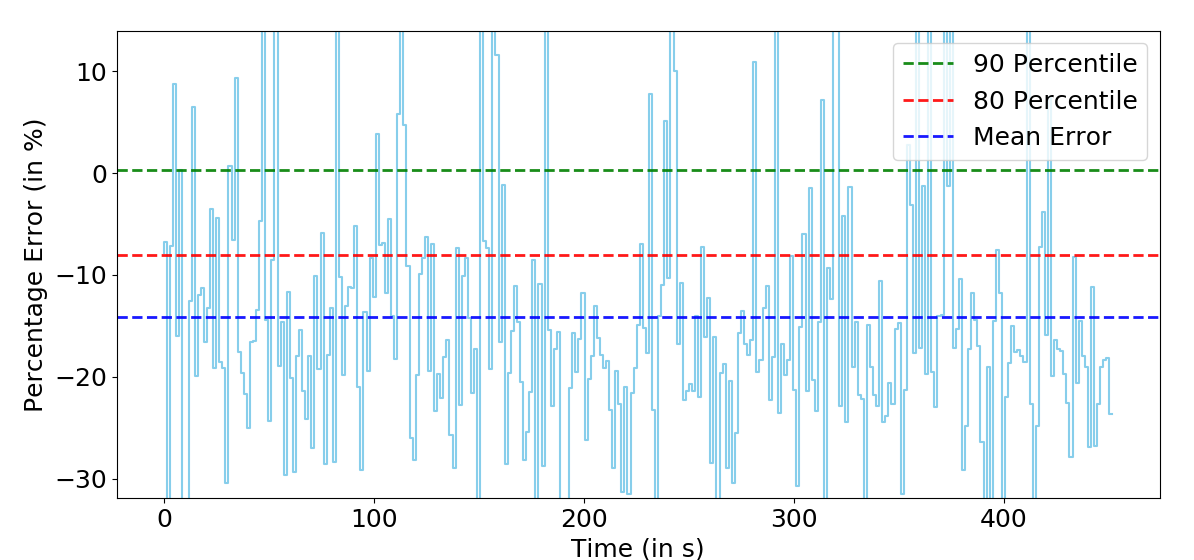
\includegraphics[width=\textwidth]{figures/sensor_error_timeline_5.png}
         \caption{Timeline on Moto Z3}
         \label{fig:sensor_error_timeline}
     \end{subfigure}
     \hfill
\fi

\begin{minipage}{0.48\columnwidth}
\begin{subfigure}[b]{\textwidth}
         \centering
         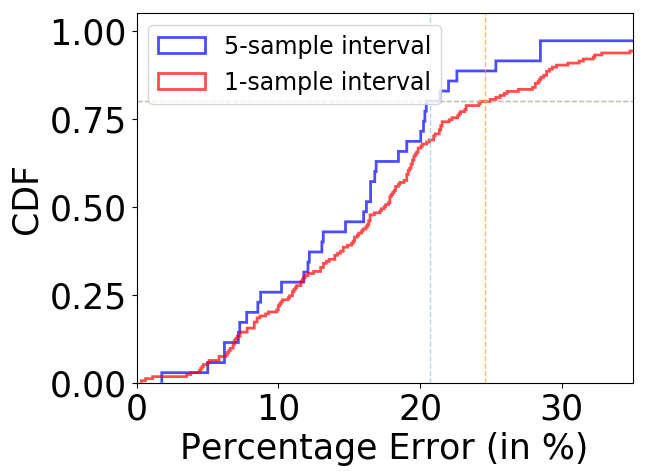
\includegraphics[width=\textwidth]{figures/sensor_error_cdf.png}
         % \caption{CDF for Moto Z3}
%         \label{fig:sensor_error_cdf_motoz3}
     \end{subfigure}
     
  \if 0
  \begin{subfigure}[b]{0.46\columnwidth}
         \centering
         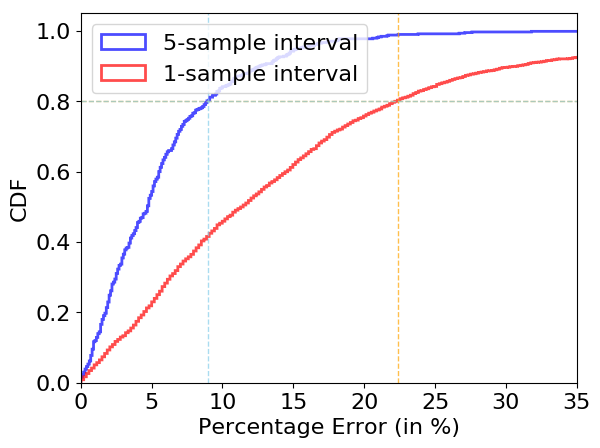
\includegraphics[width=\textwidth]{figures/sensor_error_cdf_nexus6.png}
         \caption{CDF for Nexus 6}
         \label{fig:sensor_error_cdf_nexus6}
     \end{subfigure}
  \fi
  \caption{Power sensor reading error relative to power monitor reading
        for the YouTube for Moto Z3.
        % In CDF, the orange line represents the 80 percentage for 1 sample and blue line represents for 5 sample
        }
        \label{fig:sensor_error}
        \vspace{-0.1in}
\end{minipage}
\hfill
\begin{minipage}{0.48\columnwidth}

    \centering
    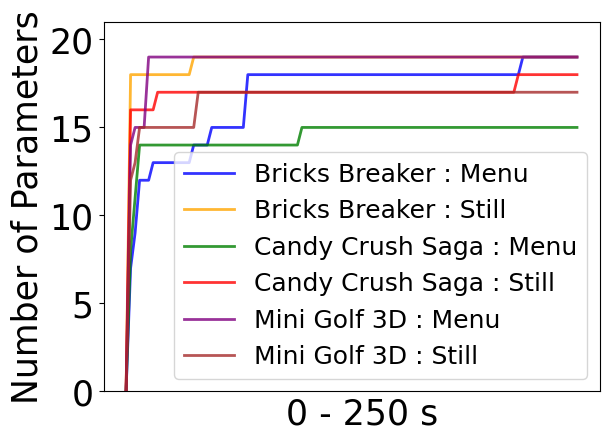
\includegraphics[width=\textwidth]{figures/004_Pixel4_cummulative_macro_parameters.png}
    \vspace{-0.1in}
    \caption{The cumulative number of unique parameters over app run duration on Pixel 4.}
    \label{fig:number_parameters_vs_duration}
    \vspace{-0.1in}
\end{minipage}
\end{figure}


 
To validate the energy counter reading accuracy comparing it with the high-fidelity 
external power monitor readings as the ground truth,
we generated a 250-second run with the YouTube app while the device is connected to the power monitor.
We chose YouTube as it is a popular app and exhibits significant power variations during its run.

%{\bf Findings}
%% 3. Explain power sensor is effects the accuracy of the equations
%Figure~\ref{fig:sensor_error} shows the timeline and the CDF for the sensor error.
\if 0
Figure~\ref{fig:sensor_error_timeline} shows the percentage error of the estimated energy
for 1-sample intervals (1.4s) based on power sensor reading over the 500s app run for Moto Z3.
We observe that \comment{for 89.7\% of the intervals the power sensor reading underestimates the energy drain compared to the power monitor reading.}
\fi

Figure~\ref{fig:sensor_error} shows the CDF for the absolute percentage error on Moto Z3
for 1-sample and for 5-sample intervals (7s). 
We plot the error for 5-sample intervals to see if averaging out over 5 samples can reduce the 
power sensor reading error.
% since if so we can set up an equation for each 5-sample interval as opposed to each 1-sample interval.
However, we see that the average error for 5-sample intervals, 15.84\%,
is only slightly better compared to 1-sample intervals of 19.01\%, and
the 80th percentile errors are 20.52\% and 24.18\% and median errors are 
16.76\% and 17.99\%., respectively.
\if 0
% , and the 80th percentile errors are 24.03\% and 21.10\%, respectively.
% Nexus 6
Figure~\ref{fig:sensor_error_cdf_nexus6} shows the CDF for the absolute percentage error
for 1-sample intervals (175 ms) and for 5-sample intervals (875 ms) for Nexus 6.
However, we see that the average error for 5-sample intervals, 7.21\%,
is lower than for 1-sample intervals of 19.06\%, and
the 80th percentile errors are 9.89\% and 26.60\%, respectively.
\comment{We observe that the sensor is about 3 times lower in Nexus 6 as compared to Moto Z3
for 1 sample interval is due to the interval of Nexus 6 being 8 times shorter than Moto Z3.
Suggesting that the low sampling rate of the sensor is the cause of the error.}
\fi
Such high error suggests that the built-in power sensor readings available on today's Android phones 
are not suitable for self power model derivation. 
Thus we conduct our SPMD verification study by using the external Monsoon power monitor to generate the 
power draw ground truth. 

\if 0
{\bf Reason }
%% 5. Reasons for the inaccuracies in power sensor
The high inaccuracy of the power sensor could be attributed to mainly 2 reasons.
\begin{itemize}
    \item {\bf Noise: } The power management circuit and it's location in the device is susceptible to noise due to the electronic circuitry involved in it.
    It can be argued that, the noise can be reduced by taking a longer interval which might average out the effect of noise, but from our finding we find that this approach is not effective.
    
    \item {\bf Low Sampling rate: } The power sensor generate a new value every 1.4 seconds interval in moto Z3.
    This greatly inhabits use of the power sensor to gather instantaneous current. 
 \end{itemize}
\fi


% The Monsoon power monitor has a sampling rate of 5 KHz  and has been widely used as the ground truth in smartphone power modeling and energy drain studies. 


\subsection{How to Set up Equations?}

The basic SPMD methodology does not specify how to set up systems of equations for the regression solver. Since SPMD is "in-situ", \ie deriving all the power model parameters experienced during a given app run,
in principle we need to create equations those can cover the entire app run duration.
Given an app run of duration $T$, 
we can potentially chop it into $N_s$ equal-sized intervals,
and set up $N_e$ equations per each interval, each covering a duration of $t_e$ of the app run, \ie
\begin{eqnarray}
T = N_s \cdot N_e \cdot t_e
\end{eqnarray}
%
Thus, setting equations for SPMD has two degrees of freedom: 
(1) How many systems of equations $N_w$ shall we create for an app run? 
(2) How many equations $N_e$ shall we create for each interval?
Our verification study explores how the two degrees of freedom can 
help us to improve the diversity for the systems of equations. 


%%%%%%%
\subsection{How to Validate Models from SPMD?}

Since the motivation of SPMD is to capture power model's dependence on app usage, SPMD is fundamentally different compared to learning in TPMD as the goal is not to train a model based on training data from some app run that will predict well the testing data for a different app run. Rather, the goal of SPMD is to generate the power model that best fits a given app run. However, this also raises a fundamental challenge in terms of how to validate the derived model as we generally do not have the ground-truth power model for a given app run. 

{ 
In our verification study, we apply a three-pronged criteria to determine whether the derived SPMD  model is considered acceptable: 
(1) The trend of the model parameters derived should appear similar to the model derived using TPMD. For example, they should be positive, follow monotonicity (\eg CPU power should grow with higher frequency), and the GPU Idle power should be less than the GPU Busy power;
(2) The specific values of the parameters should be within a threshold of their counterparts if compared with the TPMD derived model parameters. The threshold could be based on empirical evidence, \eg from the power state variation study in \S\ref{sec:primer}.
(3) We apply conventional training-testing validation by extracting interleaved training and testing data in a given app run to compare the fitting error for the training and testing data. 
}

%%%%%%%
\subsection{Aligning Power Monitor with Linux event trace}
% \begin{figure*}
%     \centering
%      \begin{subfigure}[b]{0.15\textwidth}
%          \centering
%          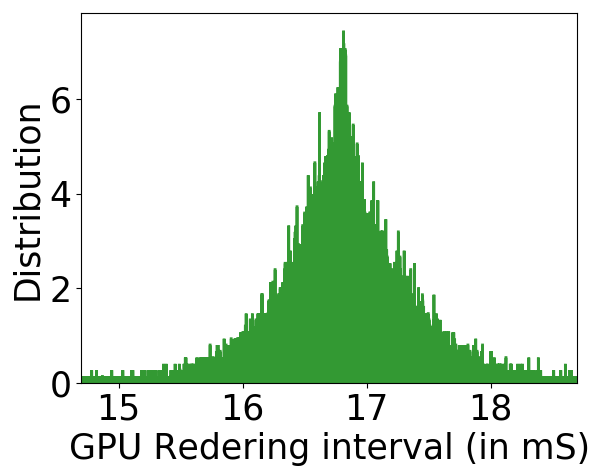
\includegraphics[width=\textwidth]{figures/distribution_interval_bricksbreaker_intro.png}
%          \caption{Bricks Breaker Intro scenario}
%      \end{subfigure}
%           \begin{subfigure}[b]{0.15\textwidth}
%          \centering
%          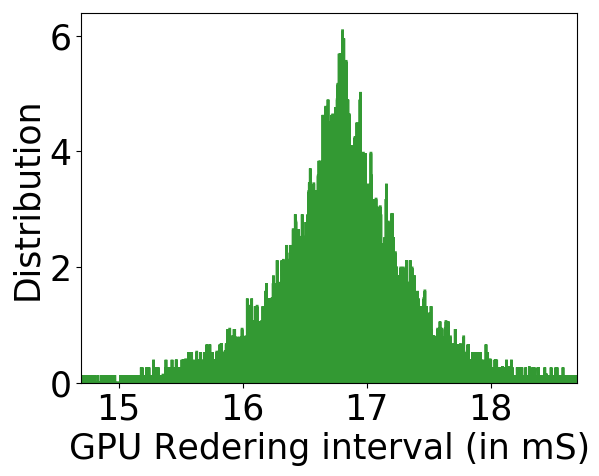
\includegraphics[width=\textwidth]{figures/distribution_interval_bricksbreaker_still.png}
%          \caption{Bricks Breaker Still scenario}
%      \end{subfigure}
%           \begin{subfigure}[b]{0.15\textwidth}
%          \centering
%          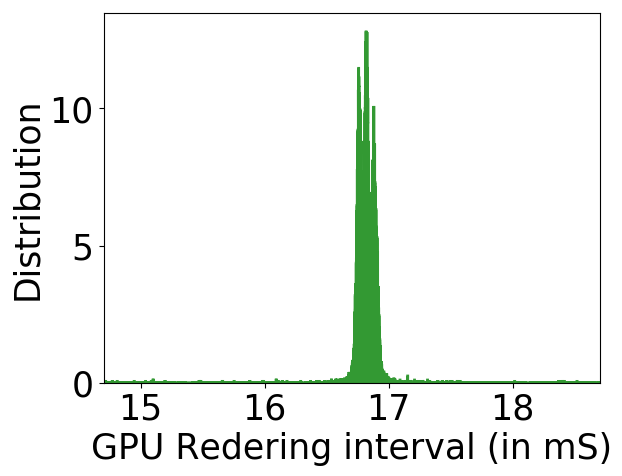
\includegraphics[width=\textwidth]{figures/distribution_interval_candycrush_menu.png}
%          \caption{Candy Crush Menu scenario}
%      \end{subfigure}
%           \begin{subfigure}[b]{0.15\textwidth}
%          \centering
%          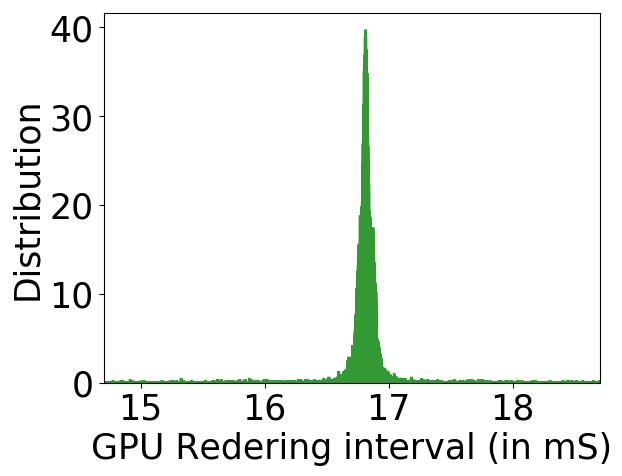
\includegraphics[width=\textwidth]{figures/distribution_interval_candycrush_tutorial.png}
%          \caption{Candy Crush Tutorial scenario}
%      \end{subfigure}
%           \begin{subfigure}[b]{0.15\textwidth}
%          \centering
%          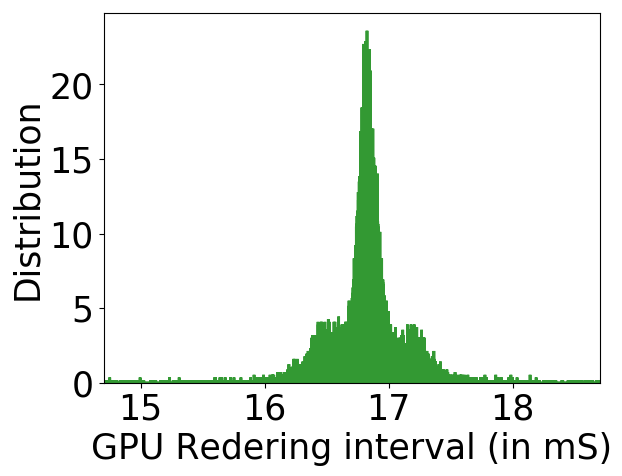
\includegraphics[width=\textwidth]{figures/distribution_interval_pottery_intro.png}
%          \caption{Pottery Intro scenario}
%      \end{subfigure}
%           \begin{subfigure}[b]{0.15\textwidth}
%          \centering
%          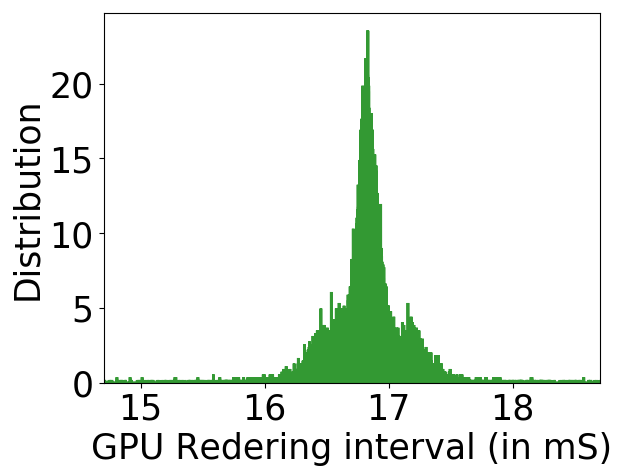
\includegraphics[width=\textwidth]{figures/distribution_interval_pottery_create.png}
%          \caption{Pottery Create scenario}
%      \end{subfigure}
%      \caption{Distribution for GPU redering interval}
%     \label{fig:distribution_gpu_interval}
% \end{figure*}
A modern smartphone on an average can generate 60 frame per second. 
From the event trace we found that the time taken to generate frames by the GPU can vary.
% Figure~\ref{fig:distribution_gpu_interval} shows the rendering interval spread
% for the 6 app scenarios collected from event trace.
The standard deviation to generate frames is found to be in  the range of 0.37 to 1.51 ms.
Figure~\ref{fig:power_trace_candycrushturorial} shows a typical rendering interval.
We first mark the rising edge on the power monitor trace as the start of the interval and 
the fall edge as the end of the GPU Active-busy state.
We choose a 50 interval window from the middle of the power monitor trace which has lowest standard deviation
for both the total rendering interval as well as GPU Active busy duration.
Then, from the event trace we use a sliding window to find out the window 
which scales best to those 50 windows of the power monitor  .
\comment{Further, for micro and nano analysis, on a per rendering interval basis,
we scale the rendering interval duration from power monitor trace to match that of the rendering
duration of the event trace interval per interval basis.}
% We choose a 50 interval window which we slide across 10 seconds in the middle of the trace.
% The cost function chosen is the L1-norm of the standard deviation of the total interval and
% the GPU Active-busy interval. We choose the 50 interval which has the least standard deviation.
% To align it with the event trace, we use L2 norm of the difference in the total interval
% and GPU Active-busy interval over a sliding window. 
\section{Experimental Setup}
\label{sec:etup}


%% 1. Explain the apps used
%% 2. Explain the device used

% We carried our SPMD on three phones with fairly diverse hardware.
% Moto Z3 is a representative of recent phone.
% It has a Kryo Qualcomm SOC~\cite{snapdragon835} based on the big.LITTLE architecture
% with 4 LITTLE cores (22 frequencies) and 4 big cores (31 frequencies), and
% an Adreno 540 GPU which can run at 7 different frequencies.
 
% In contrast, the Nexus 6 was a representative of the generation before
% the big.LITTLE architecture, with a Krait Qualcomm SOC~\cite{snapdragon805} that
% has 4 cores which can independently operate at 18 different frequencies, and
% an Adreno 420 GPU  which can run at 5 different frequencies.

% In our experiments, we simplified the SPMD modeling task by turning off the LITTLE cores on Moto Z3
% % for all our experiments, hence all our results are based on big cores.
% which reduces the number of parameters in the modeling equations.
% As we will see below, even with this simplification, making SPMD to work is already difficult. 

% Since we focus our SPMD experiments on two phone components, the CPU and GPU,
% we used a set of {three} popular game apps which are known to predominantly
% use only the CPU and GPU. The apps have diverse GPU and CPU utilization. 
% For example, the average GPU utilization is 38.0\% for Pottery,
% 25.92\% for Candy Crush Saga and 16.0\% for Bricks Breaker on Moto Z3.

We carried our SPMD on three phones.
Pixel 2 and Moto Z3 has a Kryo Qualcomm SOC Snapdragon 835~\cite{snapdragon835} and Pixel 4 has Snapdragon 855~\cite{snapdragon855} which are based on the big.LITTLE architecture.
Pixel 2 and Moto Z3 has 22 LITTLE core and 31 big core frequencies, whereas Pixel 4
has 19 LITTLE core and 17 big core frequencies.
The SOC for Pixel 2 and Moto Z3 has an Adreno 540 GPU which can run at 7 different frequencies 
and 
Pixel 4 has Adreno 640 GPU which can run at 5 different frequencies.

For our experiments, we simplified the SPMD modeling task by turning off the LITTLE cores on Moto Z3
% for all our experiments, hence all our results are based on big cores.
which reduces the number of parameters in the modeling equations.
As we will see below, even with this simplification, making SPMD to work is difficult. 
Since we focus our SPMD experiments on two of the phone components, the CPU and GPU,
we used a set of {three} popular game apps which are known to be predominantly
using only the CPU and GPU. We found that the apps have diverse GPU and CPU utilization. 
For example, the average GPU utilization is 38.0\% for Mini Golf 3D,
25.92\% for Candy Crush Saga and 16.0\% for Bricks Breaker on Moto Z3.
(Utilisation not final yet.)
We further consider two scenarios from each of these apps,
as listed in Table~\ref{tab:app_scenario_description}.

\begin{table}[tp]
    \centering
    \caption{App scenario description.}
    \vspace{-0.1in}
    {\small
    \begin{tabular}{|p{15mm}|p{12mm}|p{46mm}|}
    \hline
    \multicolumn{1}{|c|}{App} & \multicolumn{1}{c|}{Scenario} & \multicolumn{1}{c|}{Description} \\
    \hline
         \multirow{2}{15mm}{Bricks Breaker} & Menu & Menu page\\
         \cline{2-3}
         & Still & Game running without any input \\
         \hline
         \multirow{2}{15mm}{Candy Crush Saga} & Menu & Menu Page\\
         \cline{2-3}
         & Still &  Game running without any input \\
         \hline
         \multirow{2}{15mm}{Mini Golf 3D} & Menu & Menu Page \\
         \cline{2-3}
         & Still &  Game running without any input \\
        \hline
    \end{tabular}
    }
    \label{tab:app_scenario_description}
    \vspace{-0.1in}
\end{table}

We generated a 250-second run for each of the app scenario with the phone attached to the power monitor.
For
the three phones Pixel 2, Moto Z3 and Pixel 4, we kept the screen dark and removed its constant power draw of 43mA, 57mA and 78mA respectively
from the power monitor measurement to set up the equations. 
For each scenario we left the app running without any user inputs.

% \paragraph{Aligning power trigger trace with power monitor readings}
% When readings from the Monsoon external power monitor, either as ground truth in model accuracy calculation or as the left-hand-side (LHS) value of the modeling equations, 

Since the Monsoon power monitor has a separate clock and thus clock drifts from that of the phone, we need to align the time of power monitor  power readings with the timing of the data we collected on the phone.
To do this, we used a microbenchmark by generating a 5-second CPU burst known as a beacon,
and align the time of the CPU utilization surge in the event trace with the time of the corresponding square wave in the power monitor readings.

% The results we observed from our experiment can be easily extended by including corresponding triggers for the case while all the cores are running .

Finally, we found that the findings for the three phones are  very similar.
% We thus moved all the results for Nexus 6 
% to~\cite{longversion} due to page limit.

% \section{Per-Component SPMD on Modern Phones}
% \label{sec:evaluation}

% In this section, we present the experience with trying to make SPMD work
% on two modern phones. We show even when focusing on only two phone components, CPU and GPU, 
% applying SPMD faces a number of fundamental challenges. 



\section{Component-wise SPMD at Macro Scale}
\label{sec:modelling_macro}

% This cause the app to render the same frames.
% \comment{The model parameters are dependant on the usage, i.e. CPU parameter is dependent on the amount of memory operations and GPU depends on the complexity of the frames rendered. Our assumption is that With the same frames getting rendered, the model parameters remains constant. }
%% 2. How equations are generated

We first explore SPMD at macro-scale, \ie setting one equation for an interval of  1 to a few seconds order,
based on two justifications.
First, the power monitor reading resolution of 0.2ms allows us to
have accurate energy (average power draw) readings with 1 second granularity.
Second, since the GPU typically goes through the Busy and Idle states at least once
in every 16.7ms, using intervals of 1 to a few seconds 
allows averaging out potentially different GPU and CPU usage over 60 or more such rendering intervals.

\begin{figure*}[tp]
    \centering
    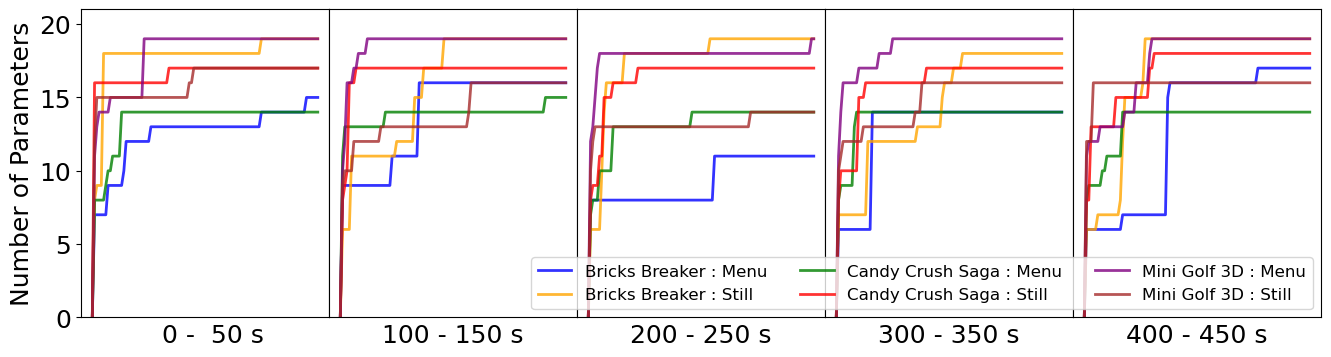
\includegraphics[width=\textwidth]{figures/004_Pixel4_cummulative_parameters.png}
    \vspace{-0.1in}
    \caption{The cumulative number of unique parameters over app run duration in five 50-second segments on Pixel 4. Fixing the x axis.}
    \label{fig:number_parameters_vs_duration_100s}
    \vspace{-0.1in}
\end{figure*}

\paragraph{How Many Systems of Equations?}
\label{subsec:relation}
Since our app run duration  are of 250 seconds each, under macro-scale SPMD  considering an interval $t_e$  between 1s to 5s, 
we can have between 100 to 250 equations.
To explore how many equations should be used,
we first measure how the number of unique model parameters varies with of the app run duration . 

Figure~\ref{fig:number_parameters_vs_duration} shows 
the cumulative number of unique power model parameters for Pixel 4 over a 250-second app run duration
for the six app scenarios . We make the following observations.
(1) The number of unique model parameters increases with the app run duration, reaching a maximum of 15 (for the Candy Crush Saga Menu scenario) to 19 for (the Mini Golf 3D Menu scenario). 
%over 500 seconds for the six app scenarios. 
(2) While the GPU stayed at one frequency and contributed 2 parameters (Busy and Idle power in that frequency) for all the 6 app scenarios,the remaining 13 to 17 are CPU core model parameters.
Similar trends are also observed for the other two  phones.

Figure~\ref{fig:number_parameters_vs_duration} does not show 
the number of unique model parameters in the smaller segments of the app run.
To see this, we plot in Figure~\ref{fig:number_parameters_vs_duration_100s} the 
cumulative number of unique model parameters over  each of 50 seconds time segment , 
for the 6 app scenarios.
We see that the curves for all of the 5 ,50-second segments look very similar, 
suggesting the apps' usage of both the CPU and GPU are similar. 
However, the total number of unique model parameters in each of the 50-second segment
may be lower when compared with the 250-second interval.
For example,on Pixel 4 with Bricks Breaker Menu  the number of parameters
for 0-250s interval is 18 and whereas for the 5 smaller segments number of parameters reduces to 15, 16, 11, 14 and 17.
This suggests that creating a system of equations for the smaller intervals 
may have fewer unknowns depending on the app scenarios.

\cut{ 
\begin{figure}[tp]
    \centering
    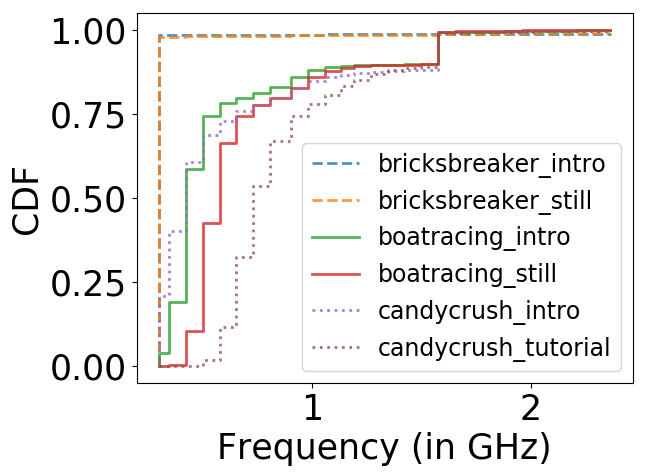
\includegraphics[width=0.65\columnwidth]{figures/cdf_frequency_residence.png}
    \vspace{-0.1in}
    \caption{CDF of the total time spent in each CPU frequencies for 6 app scenarios.}
    \label{fig:cdf_frequency_residence}
    \vspace{-0.1in}
\end{figure}

Finally, to understand how the utilization of different model parameters vary,
we plot in Figure~\ref{fig:cdf_frequency_residence} 
the CDF of the percentage of the total time (250 seconds) spent in each CPU core frequency for the six scenarios. We see the utilizations are uneven: the top 5 parameters in each app scenario
account for 75.20\% to 98.76\% of the total app run duration across the 6 app scenarios.
In contrast, the utilization of the single GPU frequency experience in each app scenario 
varies between 14.72\% and 64.51\%.
}

\begin{figure*}[tp]
    \centering
     \begin{subfigure}[b]{0.32\textwidth}
         \centering
         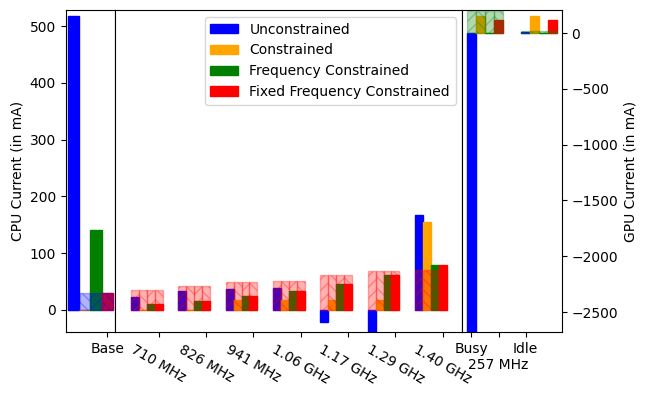
\includegraphics[width=\textwidth]{figures/004_Pixel4_bricksbreaker_menu_50_1_equations.png}
         % \caption{500 equations with 1 second equation interval}
         \label{fig:number_parameters_vs_duration_100s_0}
     \end{subfigure}
    \begin{subfigure}[b]{0.32\textwidth}
         \centering
         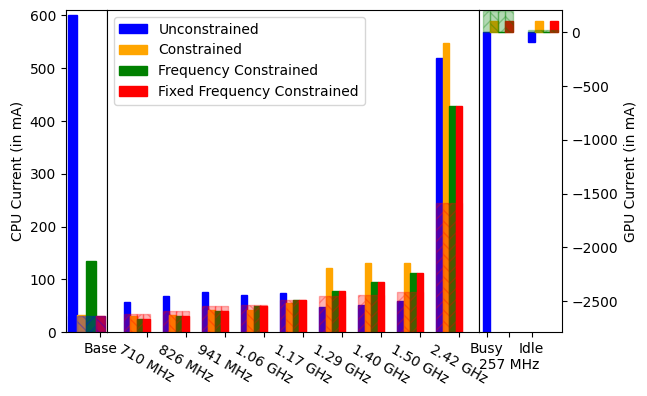
\includegraphics[width=\textwidth]{figures/004_Pixel4_bricksbreaker_menu_250_1_equations.png}
         % \caption{250 equations with 2 seconds equation interval}
         \label{fig:number_parameters_vs_duration_100s_100}
     \end{subfigure}
    \begin{subfigure}[b]{0.32\textwidth}
         \centering
         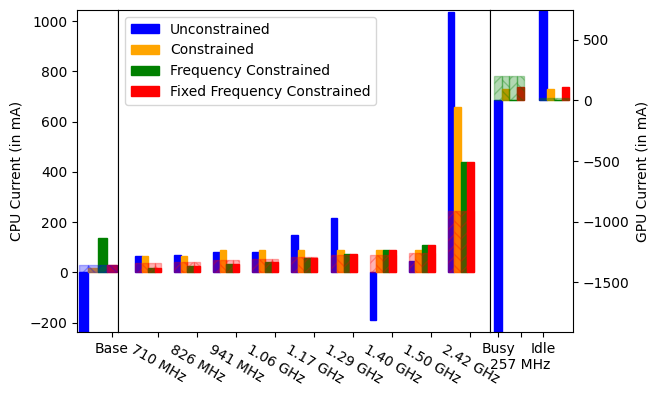
\includegraphics[width=\textwidth]{figures/004_Pixel4_bricksbreaker_menu_250_5_equations.png}
         % \caption{100 equations with 5 seconds equation interval}
         \label{fig:number_parameters_vs_duration_100s_200}
     \end{subfigure}
     \hfill
         \centering
     \begin{subfigure}[b]{0.32\textwidth}
        \centering
    	{ \scriptsize
    	\begin{tabular}{ | l | c | c | c | c | c | c | }
    		\hline
    		     & \multicolumn{6}{ c|}{Error for each App Scenarios (in \%)}\\
    		\cline{2-7}
                    Model & \rot{B. Menu} & \rot{B. Still} & \rot{C. Menu} & \rot{C. Still} & \rot{M. Menu} & \rot{M. Still}  \\
    		\hline
                Unconst.             & 0.7 & 0.9 & 0.8 & 1.1 & 1.0 & 0.9 \\
                Const.               & 1.2 & 1.1 & 1.2 & 1.6 & 1.4 & 1.3 \\
                Freq. Const.         & 1.2 & 1.1 & 1.6 & 2.1 & 1.9 & 1.8 \\
                Fix. F. Const.       & 1.2 & 1.1 & 1.6 & 2.1 & 1.9 & 1.8 \\
                Classical            & 37 & 45 & 17 & 24 & 27 & 9.2 \\
    		\hline
    	\end{tabular}
    	}
	\caption{50 equations with 1 second equation interval}
    \end{subfigure}
     \begin{subfigure}[b]{0.32\textwidth}
        \centering
    	{ \scriptsize
    	\begin{tabular}{ | l | c | c | c | c | c | c | }
    		\hline
    		     & \multicolumn{6}{ c|}{Error for each App Scenarios (in \%)}\\
    		\cline{2-7}
                    Model & \rot{B. Menu} & \rot{B. Still} & \rot{C. Menu} & \rot{C. Still} & \rot{M. Menu} & \rot{M. Still}  \\
    		\hline
                Unconst.             & 0.8 & 0.7 & 1.4 & 1.4 & 1.1 & 1.2 \\
                Const.               & 1.0 & 0.8 & 1.3 & 1.5 & 1.2 & 1.3 \\
                Freq. Const.         & 1.0 & 0.9 & 1.4 & 1.8 & 1.3 & 1.4 \\
                Fix. F. Const.       & 1.0 & 0.9 & 1.4 & 1.8 & 1.3 & 1.4 \\
                Classical            & 37 & 45 & 17 & 24 & 27 & 8.5 \\
    		\hline
    	\end{tabular}
    	}
	\caption{250 equations with 1 second equation interval}
    \end{subfigure}
         \begin{subfigure}[b]{0.32\textwidth}
        \centering
    	{ \scriptsize
    	\begin{tabular}{ | l | c | c | c | c | c | c | }
    		\hline
    		     & \multicolumn{6}{ c|}{Error for each App Scenarios (in \%)}\\
    		\cline{2-7}
                    Model & \rot{B. Menu} & \rot{B. Still} & \rot{C. Menu} & \rot{C. Still} & \rot{M. Menu} & \rot{M. Still}  \\
    		\hline
                Unconst.             & 0.4 & 0.4 & 0.7 & 0.7 & 0.5 & 0.6 \\
                Const.               & 0.6 & 0.4 & 0.8 & 0.9 & 0.6 & 0.8 \\
                Freq. Const.         & 0.7 & 0.5 & 1.0 & 1.2 & 0.9 & 1.1 \\
                Fix. F. Const.       & 0.7 & 0.5 & 1.0 & 1.2 & 0.9 & 1.1 \\
                Classical            & 37 & 45 & 17 & 24 & 27 & 8.5 \\
    		\hline
    	\end{tabular}
    	}
	\caption{50 equations with 5 second equation interval}
    \end{subfigure}
    \caption{3 ways of creating the system of equations for Bricks Breaker Menu scenario on Pixel 4. (Only model parameters for 9 CPU frequencies with highest utilization are shown due to space constraint.). Showing error for all app scenarios. \comment{Fixing the negative part of the plots.}}
    \label{fig:macro_3_ways}
    \vspace{-0.1in}
\end{figure*}

Based on the above exploration, we experimented with 3 alternatives for creating the system of equations for each app scenario, by varying
the app run duration per system between 100, and 250 seconds, and
the interval  per equation between 1, and 5 seconds, while ensuring that the number
of equations per system is 50 or more.

The solutions found with  these  3 alternatives of creating systems of equations for Bricks Breaker Menu scenario on Pixel 4 are
shown in the Figure~\ref{fig:macro_3_ways}. For comparison, we present the model parameters 
derived from traditional power model derivation by hatched bars. Note that for GPU parameters 
shown for the TPMD models is derived for the specific app scenario using Figure 1. In general, models derived using TPMD are app-agnostic. Due to page limit, we omit including all the results
found for the remaining app scenarios and 
on other phones , however the findings are very similar.
% First, we observe that the ranks of the systems are more than 1 less than the number of model parameters
% when the equation covers 100 or 200 seconds, and are 1 less than the number of parameters for 500-second app duration. The reason for this is that the base power shows up in all equations which does not contribute to the rank.
First, we observed that the ranks of the system of equations  is less than the number of model parameters by more than 1. 
The reason for this is that the base power shows up in all equations which does not contribute to the 
rank. 

As expected, since the systems are under-ranked,
the model parameters output from the regression solver look very different from those found from the classic model. 
For the {\it unconstrained solver},
the parameters generated, shown in Figure~\ref{fig:macro_3_ways},
violate some basic properties:
(1) some model parameters generated are negative, \eg the the CPU component power at 1.49 GHz is -69.70 mA for 100 intervals x 1sec  and 1.62 GHz is -3116.8 mA for 50 intervals x 5sec systems, and 
(2) the CPU power draw at a lower frequency is often higher than the power draw at a higher frequency (for all the 3 systems), and 
(3) the GPU Idle power draw generated is higher than the GPU Busy power (for all the 3 systems).

For the {\it constrained solver}, while the parameters generated, shown as 
"Constrained" in Figure~\ref{fig:macro_3_ways}, are all
positive and no more non-decreasing with increasing frequencies, the CPU power parameters
still do not satisfy the monotonicity property; the parameters for consecutive frequencies
often stay the same. For example, for the Bricks Breaker Intro scenario, 
the CPU power stays at 42.02 mA for 4 of the frequencies from 710 MHz to 1.05 GHz and again remains at 75.35 mA for 5 of the frequencies from 1.29 GHz to 1.61 GHz for the 50x5 system.

For Frequency-constrained solver,  the parameters generated, shown in in Figure~\ref{fig:macro_3_ways}, look very much similar to those in the classic model, but 
the base power draw ranges between 101.1 mA to 108.3 mA, 
which is over 3.3 times higher than their counterpart of 30.12 mA observed in the classic model.

% 41.36 mA, 33.98 mA and 30.12 mA for Pixel 2, Moto Z3 and Pixel 4
To overcome the under-rank problem, we fixed the base power to  the  constant value of 30.12 mA as in case of classic model which makes the rank equal to the  number of parameters for 
the two systems with 250-second duration, 250x1 and 50x5.  
% in the rows labeled "Fix-Freq-Constr.",
With this approach ,the parameters generated by the solver,only changed slightly; the solver splited the excessive base power and shifted it into the GPU 
Busy and Idle power and the trend of all the parameters now look similar to those observed in the classic model. 
% 
% \comment{However, the specific model parameters (excluding the base power) 
% differ from those in the classic model in two major ways.
% % (1) the individual CPU power parameter values in the two systems
% % 500x1 and 100x5 are between 0\% and 21.35\% lower than
% % their counterparts in the classic model.
% (1) the individual CPU power parameter values in the two systems are 
% 11.27\% to 96.96\% lower for 500x1 and 11.84\% to 96.78\% lower for 100x5 than
% their counterparts in the classic model.
% (2) The GPU Busy and Idle powers are identical, when the GPU Idle power is supposed to be 4$\times$ lower than the GPU Busy power.  
% }


\if 0
We make the following observations.
(1) The CPU power parameter now increases with the frequency similarly as in the classical model
and achieves between 0.55\% and 3.46\% Least Square Fitting error, 
which are lower than the error of between 5.78\% and 10.74\% archived by 
the classic model, for the four app scenarios. 
(3) However, the specific parameter values at individual frequencies differ significantly from their counterparts in the classical model. For example, 
the CPU power for 1.65 GHz is 76.23 mA in the classical model
but 28.84 mA and 44.19 mA by SPMD for the Boat Racing Intro and Candy Crush Saga Intro scenarios, respectively. Similarly, the base power ranges between 88.73 mA to 242.3 mA for the four scenarios
but is only 27.86 mA in the classic model. 
Further, the GPU power parameters are significantly underestimated: the Busy parameter under 342 MHz
ranges between 0 mA and 168.8 mA  for the two scenarios of Boat Racing but are 253.7 mA and 358.0 mA in the classic model, respectively.
\fi
% \questionaj{This is because of unconstrained GPU. Does physics inform us about any constraints for GPU other than just monotonicity.}

\paragraph{Parameters for all app scenarios.}
Using the 250x1 system of equations, we applied the Fix-Freq-Constr. version of SPMD 
to all the 6 app scenarios. Figure~\ref{fig:macro_freq_constr} shows that the model parameters generated with Fix-Freq-Constr 
suffer simillar two problems as observed in the case of the Boat Racing Intro scenario.

\begin{figure*}[tp]
    \centering
     \begin{subfigure}[b]{0.32\textwidth}
         \centering
         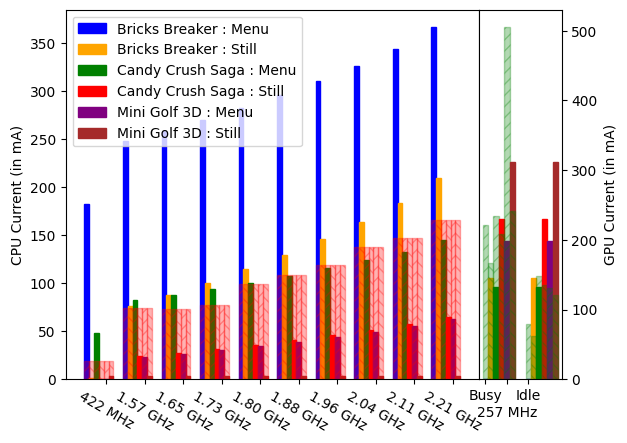
\includegraphics[width=\textwidth]{figures/002_Pixel2_250_5_macro_equations.png}
         \label{fig:number_parameters_vs_duration_100s_0}
     \end{subfigure}
    \begin{subfigure}[b]{0.32\textwidth}
         \centering
         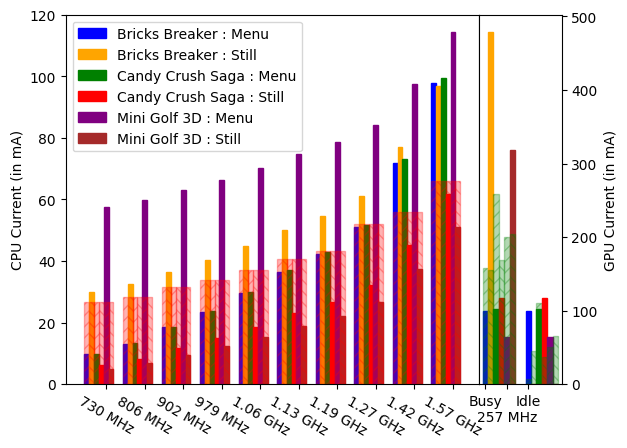
\includegraphics[width=\textwidth]{figures/003_MotoZ3_250_5_macro_equations.png}
         \label{fig:number_parameters_vs_duration_100s_100}
     \end{subfigure}
    \begin{subfigure}[b]{0.32\textwidth}
         \centering
         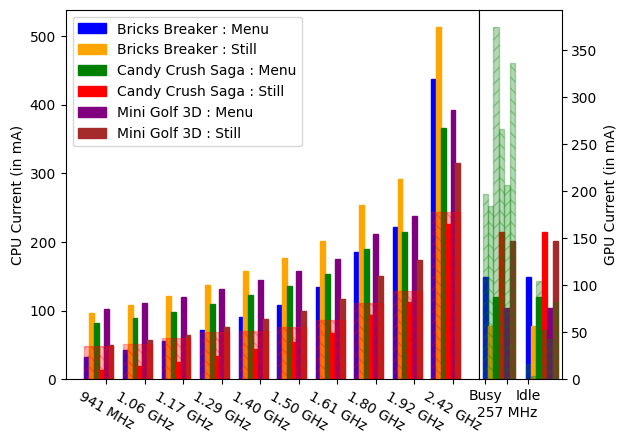
\includegraphics[width=\textwidth]{figures/004_Pixel4_250_5_macro_equations.png}
         \label{fig:number_parameters_vs_duration_100s_200}
     \end{subfigure}
     \hfill
     \centering
     \begin{subfigure}[b]{0.32\textwidth}
        \centering
    	{ \scriptsize
    	\begin{tabular}{ | l | c | c | c | c | c | c | }
    		\hline
    		     & \multicolumn{6}{ c|}{Error for each App Scenarios (in \%)}\\
    		\cline{2-7}
                    Model & \rot{B. Menu} & \rot{B. Still} & \rot{C. Menu} & \rot{C. Still} & \rot{M. Menu} & \rot{M. Still}  \\
    		\hline
                Fix. F. Const.       & 0.9 & 1.1 & 1.2 & 0.6 & 0.8 & 0.7 \\
                Classical            & 18 & 28 & 13 & 3.4 & 45 & 6.0 \\
    		\hline
    	\end{tabular}
    	}
	\caption{Pixel 2}
    \end{subfigure}
         \begin{subfigure}[b]{0.32\textwidth}
        \centering
    	{ \scriptsize
    	\begin{tabular}{ | l | c | c | c | c | c | c | }
    		\hline
    		     & \multicolumn{6}{ c|}{Error for each App Scenarios (in \%)}\\
    		\cline{2-7}
                    Model & \rot{B. Menu} & \rot{B. Still} & \rot{C. Menu} & \rot{C. Still} & \rot{M. Menu} & \rot{M. Still}  \\
    		\hline
                Fix. F. Const.       & 1.8 & 0.3 & 2.6 & 0.4 & 0.2 & 26 \\
                Classical            & 39 & 11 & 31 & 19 & 5.9 & 39 \\
    		\hline
    	\end{tabular}
    	}
	\caption{Moto Z3}
    \end{subfigure}
         \begin{subfigure}[b]{0.32\textwidth}
        \centering
    	{ \scriptsize
    	\begin{tabular}{ | l | c | c | c | c | c | c | }
    		\hline
    		     & \multicolumn{6}{ c|}{Error for each App Scenarios (in \%)}\\
    		\cline{2-7}
                    Model & \rot{B. Menu} & \rot{B. Still} & \rot{C. Menu} & \rot{C. Still} & \rot{M. Menu} & \rot{M. Still}  \\
    		\hline
                Fix. F. Const.       & 0.7 & 0.5 & 1.0 & 1.2 & 0.9 & 1.1 \\
                Classical            & 37 & 45 & 17 & 24 & 27 & 8.5 \\
    		\hline
    	\end{tabular}
    	}
	\caption{Pixel 4}
    \end{subfigure}
     \hfill
    \caption{Model parameters derived by macro-scale SPMD for 50x5 system on the 3 phones. The classic models for GPU are from Figure~\ref{fig:gpu_model}. (Only model parameters for 10 CPU frequencies with highest utilization are shown due to space constraint.) Hatched bars represents the classical model coefficients.}
    \label{fig:macro_freq_constr}
    \vspace{-0.1in}
\end{figure*}

\subsection{Analysis}
We dig deeper into one of the the full-rank system, \ie 50x5, to understand why 
SPMD generates very different parameters compared to the classic model. 
\comment{
Since the rank of the system is already full, we calculated the singular values for these equations.
Table~\ref{tab:macro_singularvalues} shows that each of the system of equations has only 1 dominating singular value, 
suggesting that the matrix (formed by coefficients of unknown variables in the left-hand-side of those equations) has only one dominating direction. This indicates that all the equations are basically describing the same state of power usage, and thus lack diversity.
}
% These results suggest the equations lack diversity in terms of component usage. 

\begin{table*}[tp]
% \questionaj{Also add rank of freq-constrained case}
{\small
    \centering
    \caption{The rank and singular values for the set of equations for macro-scale "Fix-Freq.-Constr. SPMD" for 50x5 system on Pixel 4. (Top 11 singular values are shown.)}
    \vspace{-0.1in}
    \begin{tabular}{|c|c|c|c|c|c|c|c|c|c|c|c|c|c|c|c|}
    \hline
        App & Scenario & \# of Eqns. & \# of Vars. & Rank &  \multicolumn{11}{c|}{Singular Values} \\
        \hline
         \multirow{2}{15mm}{Bricks Breaker} & Menu & 50 & 18 & 17 & 6.54  & 0.37  & 0.17  & 0.10  & 0.04  & 0.02  & 0.02  & 0.01  & 0.01  & 0.00  & 0.00 \\
         \cline{2-16}
         & Still &  50 & 19 & 16 & 6.73  & 0.38  & 0.34  & 0.16  & 0.03  & 0.02  & 0.02  & 0.01  & 0.01  & 0.01  & 0.00 \\
         \hline
        \multirow{2}{15mm}{Candy Crush Saga} & Menu &  50 & 19 & 19 & 6.79  & 0.49  & 0.19  & 0.10  & 0.08  & 0.03  & 0.03  & 0.02  & 0.02  & 0.01  & 0.01 \\
         \cline{2-16}
         & Still & 50 & 17 & 17 & 6.81  & 0.52  & 0.21  & 0.10  & 0.05  & 0.05  & 0.03  & 0.02  & 0.01  & 0.01  & 0.01 \\
         \hline
        \multirow{2}{15mm}{Mini Golf 3D} & Menu & 50 & 19 & 19 & 6.41  & 1.62  & 0.47  & 0.38  & 0.18  & 0.06  & 0.03  & 0.02  & 0.02  & 0.01  & 0.01 \\
        \cline{2-16}
	     & Still & 50 & 17 & 17 & 6.46  & 0.99  & 0.34  & 0.19  & 0.11  & 0.06  & 0.04  & 0.03  & 0.02  & 0.01  & 0.01 \\
	     \hline
    \end{tabular}
    \label{tab:macro_singularvalues}
    \vspace{-0.1in}
}
\end{table*}

% \questionaj{I don't think next 2 paragraphs are necessary. Low rank 
% already established  that the model equations have little diversity}
% In addition to the low ranks of the systems of model equations under the macro-scale,
% suggesting the equations lack diversity in terms of component usage, 

In addition to lack of diversity in phone component usage which contributed 
to the sparse singular values, we found that the energy values in LHS of the equation   appear to contain 
measurement noise which further prevents the regression solver from generating meaningful solutions.
To see this, we plot the distribution of the LHS energy values of the 
equations in the two systems 250x1 and 50x5, 
% \ie the energy values for the 50 1-second intervals.
Figures~\ref{fig:y_distribution}(a)-(b) 
show the energy values for the two systems are clustered in a Gaussian distribution with standard deviation of 3.04 mA and 5.72 mA, 
each of which is less than 2.45\% compared with the mean value.
This Gaussian-like distribution suggests that the LHS values of the equations contain
measurement noise.
\comment{this is not obvious????}

\begin{figure}[tp]
    \centering
         \begin{subfigure}[b]{0.49\columnwidth}
         \centering
         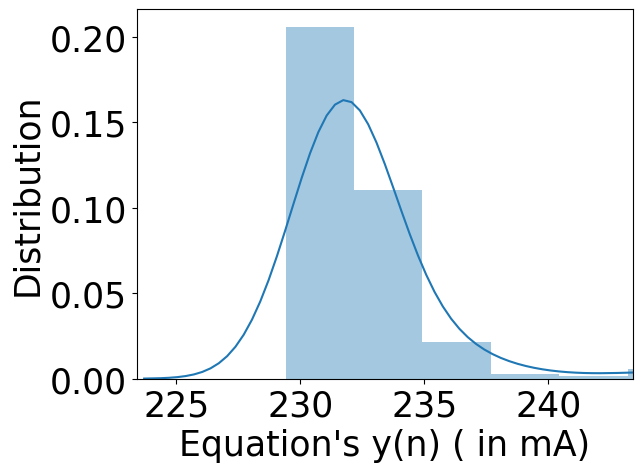
\includegraphics[width=\textwidth]{figures/004_Pixel4_bricksbreaker_menu_250_1_distribution_y_n.png}
         \caption{250 1-second equations.}
         \label{fig:y_n_boatracing_intro_1_500}
    \end{subfigure}
    \hfill
    \begin{subfigure}[b]{0.49\columnwidth}
         \centering
         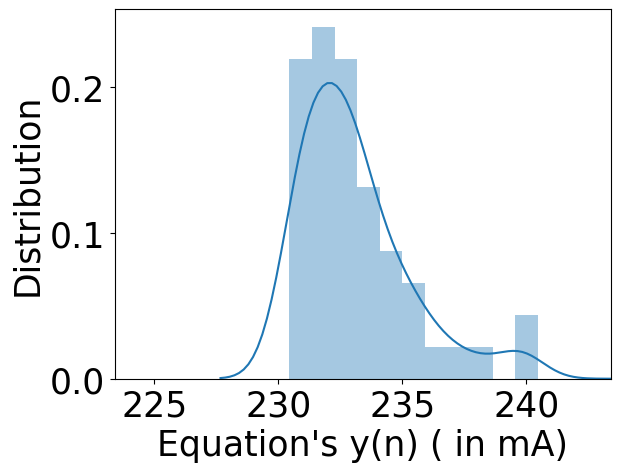
\includegraphics[width=\textwidth]{figures/004_Pixel4_bricksbreaker_menu_250_5_distribution_y_n.png}
         \caption{50 5-second equations.}
         \label{fig:y_n_boatracing_intro_5_500}
    \end{subfigure}
    \caption{Distribution of the energy terms of the
    equations for Bricks Breaker Menu scenarios on Pixel 4.}
    \label{fig:y_distribution}
\end{figure}

\if 0
Mathematically, since the small variations of the equations
all fall in a small volume of the multidimensional space, 
multiple solutions, from different constraints, 
that all have similar error, become possible as shown in Figure~\ref{fig:mutiple_equations}.

\begin{figure}[tp]
    \centering
    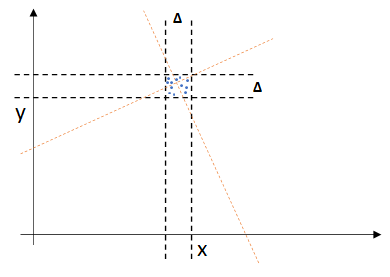
\includegraphics[width=0.70\columnwidth]{figures/mutiple_equations.png}
    \vspace{-0.1in}
    \caption{Multiple solutions (from different constraints) give similar errors due to low equation diversity.}
    \label{fig:mutiple_equations}
    \vspace{-0.1in}
\end{figure}
\fi



\if 0
\begin{figure}[hp]
    \centering
    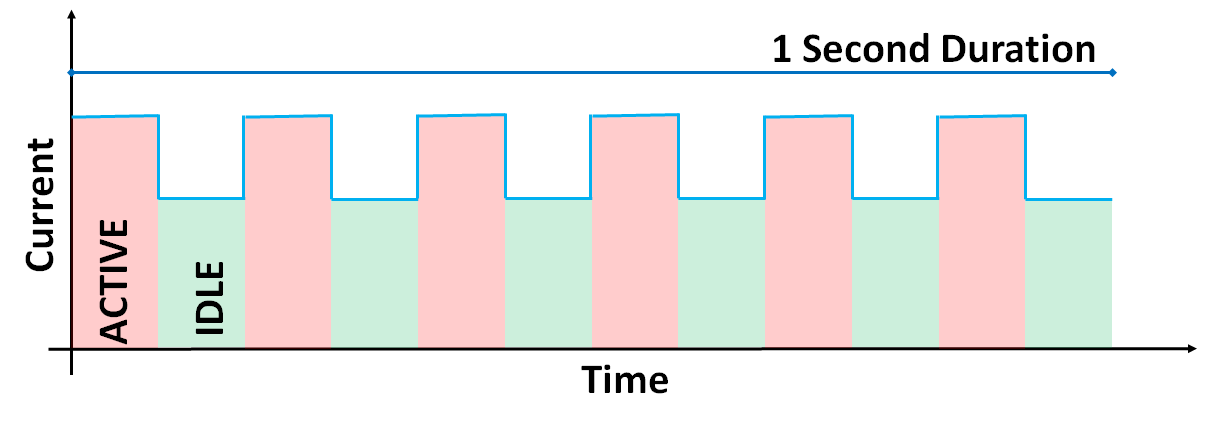
\includegraphics[width=0.95\columnwidth]{figures/coarse_grained_2.png}
    \vspace{-0.1in}
    \caption{The equations are too coarse grained}
    \label{fig:coarse_grained}
    \vspace{-0.1in}
\end{figure}
\fi

\begin{figure}[tp]
    \centering
    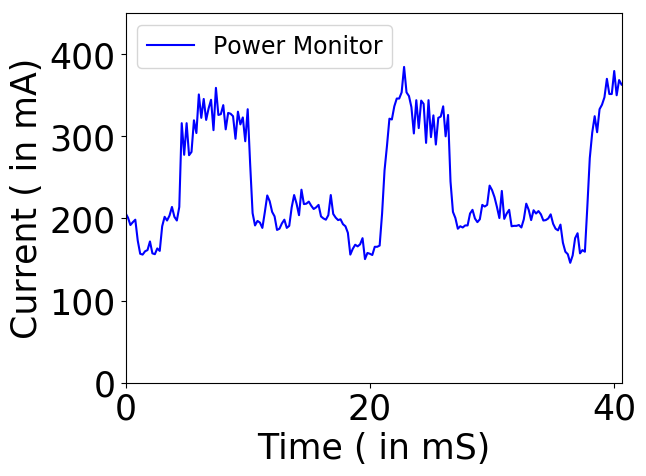
\includegraphics[width=0.50\columnwidth]{figures/candy_crush_saga_tutorial_timeline.png}
    \vspace{-0.1in}
    \caption{A snippet of power monitor readings for Candy Crush Saga Menu scenario on Moto Z3.}
    \label{fig:power_trace_candycrushturorial}
    \vspace{-0.1in}
\end{figure}

To understand why the system of model equations for the 6 app scenarios lack diversity, 
we zoom into the power monitor readings. Figure~\ref{fig:power_trace_candycrushturorial}
shows a snippet of the power monitor readings during the Candy Crush Saga Tutorial scenario. 
We see that the power draw shows a clear repeating pattern every 16.7ms duration.
This happens due to typical game app behavior -- a game app typically
renders 60 FPS and the graphic contents rendered within each game scenario are largely similar.
As a result, aggregating the power activities within each of the one-second interval into one model equation
will result in the (set of ??) equations (for the same app scenario) looking largely similar. 

% The smartphones run at a given frames per second (with an upper limit). For Moto Z3 at max 60 frames can be displayed on the screen. Frames per second is dictated by the application running. The game apps generate frames at 60 FPS which translates to 1 frame getting rendered and displayed every 16.7 ms.
%% 6b. Explain that variation is in 16.7mS

To summarize,our experiments and analysis above suggest
that the equations created from macro-scale SPMD do not exhibit enough diversity 
and as a result the regression solver can not output meaningful solutions for the model parameters.

% to conclude that we need to dig deeper and to have much smaller equation duration for retaining state change information needed to solve the set of equations meeting our goals explained in~\S\ref{sol:goals}.
\section{Can Zooming into Smaller Time Scale Improve Diversity?}

\subsection{Per-Component SPMD at Micro-Scale}
\label{sec:modelling_micro}

%% 1. Introduction: Zooming into 16.7 ms to extract variation
%%    1a. Explain the variation in 16.7 ms: Busy and idle period
%% 2. Explain how the equations are generated
%% 3. Explain the results
%%    3a. Explain why the solution are not correct
%% 4. Provide the reason for the bad solutions: explain underdetermined equations
%%    4a. Explain 2 variable in GPU
%%    4b. Explain 2 variable in CPU
%%    4c. Explain 4 variable 2 equations
%% 5. Conclusion: Due to underdetermined equations, the solution is infeasible

The repeating app usage across rendering intervals suggests that
we need to look inside each rendering interval in order to create multiple equations those
are diverse in phone component usage. 
Figure~\ref{fig:power_trace_candycrushturorial} shows the power draw during 
two 16.7 ms intervals for the Candy Crush Saga Menu scenario.
We can observe that there are two distinctive plateaus in each single 16.7 ms interval.
The higher one is when the GPU is in the Busy state and
the lower plateau is when the GPU is in Idle state. 
These two plateaus provide us with two sub intervals for generating two diverse equations.
We denote this as {\it SPMD at micro-scale}.
% When we are generating the equations over any interval longer than 16.7ms, we inadvertently average the power and loose state change information as shown in figure~\ref{fig:coarse_grained}.

\begin{figure*}[tp]
    \centering
     \begin{subfigure}[b]{0.32\textwidth}
         \centering
         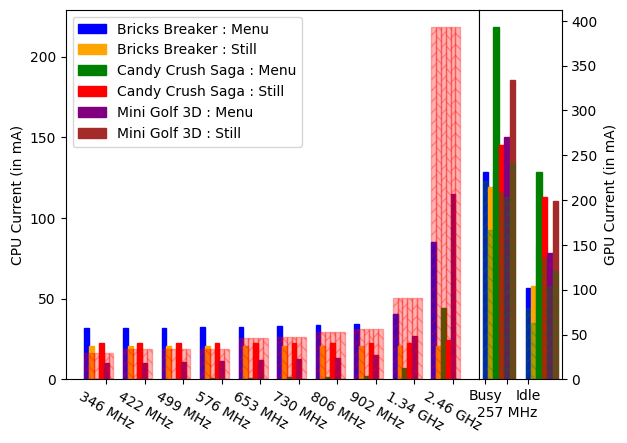
\includegraphics[width=\textwidth]{figures/002_Pixel2_16_micro_equations.png}
         \label{fig:number_parameters_vs_duration_100s_0}
     \end{subfigure}
    \begin{subfigure}[b]{0.32\textwidth}
         \centering
         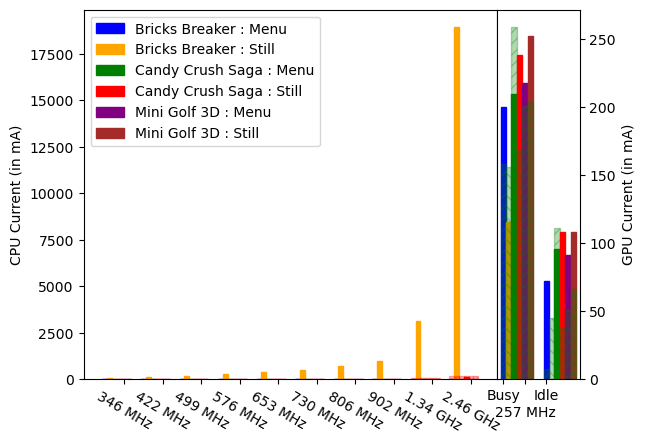
\includegraphics[width=\textwidth]{figures/003_MotoZ3_16_micro_equations.png}
         \label{fig:number_parameters_vs_duration_100s_100}
     \end{subfigure}
    \begin{subfigure}[b]{0.32\textwidth}
         \centering
         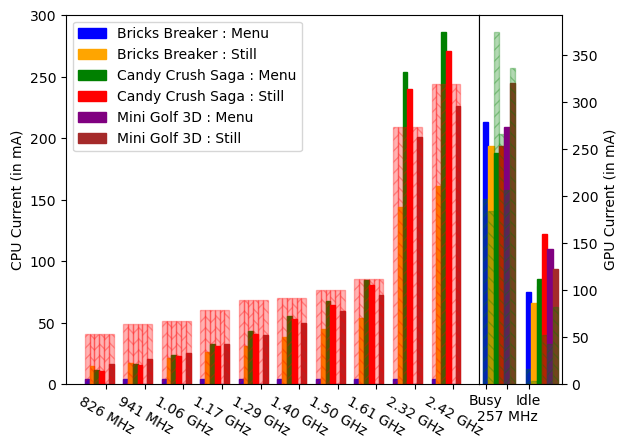
\includegraphics[width=\textwidth]{figures/004_Pixel4_16_micro_equations.png}
         \label{fig:number_parameters_vs_duration_100s_200}
     \end{subfigure}
     \hfill
     \centering
     \begin{subfigure}[b]{0.32\textwidth}
        \centering
    	{ \scriptsize
    	\begin{tabular}{ | l | c | c | c | c | c | c | }
    		\hline
    		     & \multicolumn{6}{ c|}{Error for each App Scenarios (in \%)}\\
    		\cline{2-7}
                    Model & \rot{B. Menu} & \rot{B. Still} & \rot{C. Menu} & \rot{C. Still} & \rot{M. Menu} & \rot{M. Still}  \\
    		\hline
                Fix. F. Const.       & 2.0 & 2.5 & 5.5 & 16 & 3.9 & 13 \\
                Classical            & 14 & 24 & 25 & 16 & 49 & 28 \\
    		\hline
    	\end{tabular}
    	}
	\caption{Pixel 2}
    \end{subfigure}
         \begin{subfigure}[b]{0.32\textwidth}
        \centering
    	{ \scriptsize
    	\begin{tabular}{ | l | c | c | c | c | c | c | }
    		\hline
    		     & \multicolumn{6}{ c|}{Error for each App Scenarios (in \%)}\\
    		\cline{2-7}
                    Model & \rot{B. Menu} & \rot{B. Still} & \rot{C. Menu} & \rot{C. Still} & \rot{M. Menu} & \rot{M. Still}  \\
    		\hline
                Fix. F. Const.       & 7.5 & 18 & 7.5 & 5.9 & 6.4 & 4.2 \\
                Classical            & 32 & 21 & 37 & 16 & 12 & 8.5 \\

    		\hline
    	\end{tabular}
    	}
	\caption{Moto Z3}
    \end{subfigure}
         \begin{subfigure}[b]{0.32\textwidth}
        \centering
    	{ \scriptsize
    	\begin{tabular}{ | l | c | c | c | c | c | c | }
    		\hline
    		     & \multicolumn{6}{ c|}{Error for each App Scenarios (in \%)}\\
    		\cline{2-7}
                    Model & \rot{B. Menu} & \rot{B. Still} & \rot{C. Menu} & \rot{C. Still} & \rot{M. Menu} & \rot{M. Still}  \\
    		\hline
                Fix. F. Const.       & 7.5 & 18 & 7.5 & 5.9 & 6.4 & 4.2 \\
                Classical            & 32 & 21 & 37 & 16 & 12 & 8.5 \\

    		\hline
    	\end{tabular}
    	}
	\caption{Pixel 4}
    \end{subfigure}
     \hfill
    \caption{Model parameters derived by micro-scale SPMD}
    \label{fig:micro}
    \vspace{-0.1in}
\end{figure*}

\paragraph{Methodology}
We follow the same methodology as described in \S\ref{sec:modelling_macro}
except that we generated two equations per 16.7 ms interval, one for GPU in Busy state
and the other for GPU Idle state and these correspond to the two plateaus.
As before, we fixed the base power as a constant to avoid the under-rank problem caused due to it
and use the Fix-Freq-Constrained version of the solver.


\paragraph{Findings}
In creating the two equations, we observed that there are more than two unknowns as elaborated below.
First, we observe that GPU almost never changes frequency within each 16.7ms interval,
and hence it contributes two unknowns,i.e for the GPU Busy state and Idle state power.
Second, the CPU may change frequency, potentially contributing multiple CPU power parameters.
% the active power at that multiple frequencies.
This makes the system of two equations under-determined.
%
To solve this problem, we tried to set up 2 equations 
each per interval for 2, 4, 8, 16 intervals,
% we created 8 and 32 equations for four and sixteen consecutive 16.7 ms intervals respectively.
% which typically have the same 3 unknowns as 
% the CPU ad GPU tend to stay in the same power states in generating two very similar frames.
%
% Although, we feed 4 equations into curve\_fit() to generate the solution, but they mainly
% represent only a set of 2 equations, one for GPU Active-busy and other as GPU Active-idle.
% 
Figure~\ref{fig:micro} shows the model parameters output by the regression solver for the six app scenarios on the three phones for 16 equations. The results for other 
intervals are similar and omitted due to page limit. 

We make the following observations.
(1)The power models output by the solver have LSF error
between 2.4\% to 12.8\% for Pixel 2, between 6.2\% to 15.6\% for Moto Z3 and between 2.6\% to 15.6\% for Pixel 4
(2) The individual power parameters are 1.05$\times$-1.67$\times$, 1.02$\times$-1.52$\times$, 0.94$\times$-1.44$\times$ of their counterparts  for GPU Frequency-Busy and  1.26$\times$-1.65$\times$, 0.64$\times$-4.5$\times$, 1.78$\times$-29.35$\times$ of their counterparts for GPU Frequency-Idle in the classic model for Pixel 2,Moto Z3,Pixel 4 respectively . 

% These power models are considered meaningful for use, for example, in energy accounting. 
The models are not considered acceptable as the high error suggests the models cannot capture the power state variation well. 

\paragraph{Validation}
\comment{ 
How often can we get acceptable solutions for systems of 8 equations? 
Validation of Micro SPMD using interleaved "training" and "testing" data. 
Pick 16 equations, form training data using odd equations, and testing data using even equations.
}

\if 0
(1) For most of the cases, the CPU power parameters generated are overwhelming below their
counter part in the classical model, \eg 0 mA for Boat Racing Intro with 32 equations
and close to 0 mA, \eg for Boat racing Still with 32 equations
(2) For Boat Racing Intro with 8equations, the CPU power paramaters are similar to their counterparts in the classic model, but the GPU Idle power of 161.1 mA is over 2 times higher than the corresponding 67.25 mA in the classic model. 
(3) Finally, only for two of the 12 scenarios, Bricks Breaker Intro with 8 and 32 equations, shown in bold, the power parameter seems reasonable, \ie within 50\% of their counterparts in the classic model.
\fi

\if 0
%% For Nexus 6
(3) similarly, for Nexus 6 the base power by SPMD is overestimated, 
145.2 mA and 300.7 mA for the Brick Breakers scenarios and 
419.2 mA and 413.3 mA for the Candy Crush Saga scenarios which are 7 to 21 times higher than
the 20.16 mA value in the classical model; and
(4) At 422 MHz in Bricks Breaker, 
the CPU powers are overestimated for the Intro scenario as 56.86 mA
but underestimated for the Still scenario as 8.21 mA, compare to 32.17 mA 
in the classical model.
%% 4. Provide the reason for the bad solutions: explain underdetermined equations
% Due to space constraints the detailed results are in the appendix.
\fi

\paragraph{Analysis}
To understand why some systems can generate reasonable models while other
cannot, we first plot in Table~\ref{tab:micro-rank_motoz3} the rank and top singular values for the 12 equation systems. We see that all the systems are full rank, and have sufficient number of
high singular values.  

\if 0
\begin{figure}[tp]
    \centering
    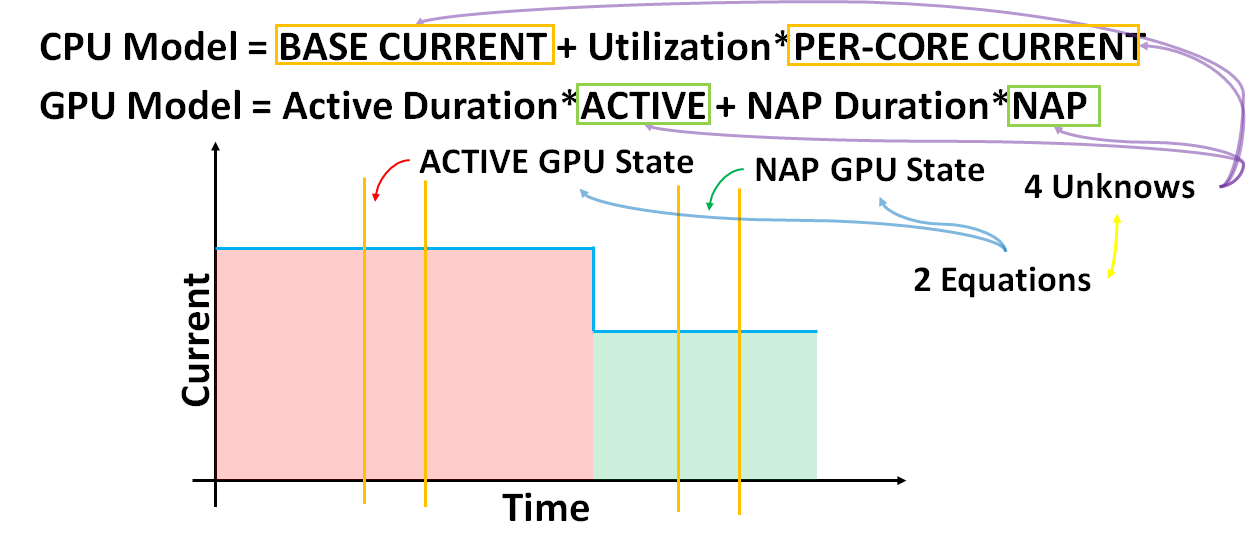
\includegraphics[width=0.95\columnwidth]{figures/underdetermined_2.png}
    \vspace{-0.1in}
    \caption{The equation are underdetermined even in 16.7 ms Micro-Scale}
    \label{fig:micro_underdetermied}
    \vspace{-0.1in}
\end{figure}
\fi

\begin{table}[tp]
{\footnotesize
    \centering
    \caption{The rank and singular values for the set of equations for micro-scale "Fix-Freq.-Constr. SPMD" for Pixel 4 for 16 equation system of equation.
    (Top 4 singular values are shown.)
    }
    \vspace{-0.1in}
    \begin{tabular}{|c|p{9mm}|p{4.5mm}|p{4.5mm}|p{4.5mm}|p{4mm}|p{4mm}|p{4mm}|p{4mm}|}
    \hline
        App & Scenario & Num. of Eqns. & Num. of Vars. & Rank &  \multicolumn{4}{c|}{Singular Values} \\
        \hline
         \multirow{2}{13mm}{Bricks Breaker} & Menu & 32 & 6 & 6 & 4.46  & 4.01  & 1.66  & 0.97 \\
         \cline{2-9}
         & Still &  32 & 6 & 6 & 4.52  & 4.02  & 1.80  & 1.01 \\
         \hline
         \multirow{2}{13mm}{Candy Crush Saga} & Menu & 32 & 7 & 7 & 5.88  & 4.02  & 3.52  & 0.56 \\
         \cline{2-9}
         & Still & 32 & 7 & 7 & 6.70  & 4.00  & 3.30  & 2.64 \\
         \hline
        \multirow{2}{13mm}{Mini Golf 3D} & Menu & 32 & 12 & 11 & 5.33  & 3.99  & 2.90  & 1.88 \\
        \cline{2-9}
	     & Still & 32 & 6 & 6 & 5.63  & 4.03  & 3.11  & 1.00 \\
	     \hline
    \end{tabular}
    \label{tab:micro-rank_motoz3}
    \vspace{-0.1in}
}
\end{table}



\begin{table}[tp]
    \centering
    \caption{Equations for the 4 consecutive 16.7 ms intervals for Bricks Breaker Menu scenario on Moto Z3.}
    {\small
    \begin{tabular}{|c|c|c|c|c|}
        \hline
             Eqn &    y(n) & \multicolumn{1}{c|}{CPU Utilization} & \multicolumn{2}{c|}{GPU Utilization} \\
        \cline{4-5}
             & (mA) & \multicolumn{1}{c|}{} & Busy & Idle \\
        \hline
                1 & 319.9 &  44\% & 100\% &   0\% \\  
                2 & 168.5 & 133\% &   0\% &  99\% \\
                \hline
                3 & 335.2 &  35\% & 100\% &   0\% \\ 
                4 & 159.8 & 131\% &   0\% &  99\% \\
                \hline
                5 & 321.4 &  86\% & 100\% &   0\% \\ 
                6 & 166.2 & 134\% &   2\% &  97\% \\
                \hline
                7 & 292.9 &  40\% & 100\% &   0\% \\ 
                8 & 162.3 & 136\% &   0\% &  99\% \\   
        \hline
    \end{tabular}
    }
    \label{tab:equations_micro}
\end{table}

Next, we take a close look at two systems, one with acceptable and one with unacceptable power parameters generated.
Table~\ref{tab:equations_micro} shows the 8 equations for 
Bricks Breaker Menu for Moto Z3 
%with 8 equations,
where equations 1, 3, 5 and 7 correspond to the GPU Busy subintervals and 
equations 2, 4, 6 and 8 correspond to the GPU Idle subintervals within the rendering intervals. 

We make two  observations:
(1) the four equations for GPU Idle subintervals, 2, 4, 6, and 8 are very similar in GPU usage
and the four equations for GPU Busy subintervals, 1, 3, 5, and 7 are very similar in GPU usage. 
(2) These two groups differ in CPU utilization which are consistent with their
the energy values on the LHS.
We see that the noise in energy values appear to dominate the diversity in CPU usage. 
For example, the CPU utilization of Eq.~.1 and Eq.~3 are 44\% and 35\%,
but their normalized energy value are 319.9 mA and 335.2 mA, respectively. 
As a result, the solver is not able to generate meaningful CPU power parameters.
\comment{
how do we explain the energy value variation
between Eq.~2 and Eq.~4  does not affect the solutions here?
}

\if 0
\comment{
Table~\ref{tab:equations_micro_bricksbreaker_still} shows the 8 equations for 
Bricks Breaker Still scenario on Moto Z3 which results in incorrect solutions, \eg CPU power of 0 mA.
We see that the noise in energy values appear to dominate the
diversity in CPU usage. 
For example, 
the CPU utilization of Eq.~.2 and Eq.~4 are 124\% and 124\%,
but their normalized energy value are 171.9 mA and 162.7 mA, respectively. 
As a result, the solver is not able to generate meaningful CPU power parameters.
}
\fi


\comment{
These results suggest while zooming into rendering intervals increased the diversity of the systems of equations - they are full rank and have good singular values, but the most of the times the solver cannot output reasonable model parameters due to energy value measurement noise. 
} \comment{not sure what to conclude here???}
\subsection{SPMD at Nano-Scale}
\label{sec:modelling_nano}

%% 1. Introduction: How to get more variations
%% 2. How to generate the equations
%% 3. Explain Alignment how power monitor is aligned with event trace
%%    3a. Explain gradient method to align 
%% 4. Explain the results
%%    4a. Explain problems in CPU Base power
%%    4b. Explain problems in per-core CPU power
%%    4c. Explain problems in GPU
%% 5. Reasons for the equation not giving correct solution
%% 6. Conclusion

Given that the component usage diversity 
seems to mainly exist within each rendering interval yet creating two equations per interval
are not enough, we next explore setting up multiple model equations, each at an even finer scale, within each 16.7ms interval. We denote this approach as {\it SPMD at nano-scale}.

\paragraph{Methodology}
%% 2. How to generate the equations
The methodology is similar to that of micro-scale SPMD, except
that instead of generating two equation per 16.7 ms interval,
we generate 16 equations, \ie one equation for every 1ms sub-interval. 
We tried 1, 2, 4, and 8 number of 16.7 ms intervals and show results for 1 interval \ie 16 equations.
Due to page limit; the other results are very similar. 

\if 0
\begin{table}[tp]
{\footnotesize
    \centering
    \caption{Normalized vector distance between 16.7 ms intervals for nano-scale SPMD for Moto Z3.}
    \vspace{-0.1in}
    \begin{tabular}{|c|c|c|c|}
    \hline
        App & Scenario & Mean & Standard deviation \\
        \hline
         \multirow{2}{20mm}{Boat Racing} & Into & 0.00 & 0.07 \\
         \cline{2-4}
         & Still & 0.00 & 0.03 \\
         \hline
         \multirow{2}{20mm}{Bricks Breaker} & Into & 0.00 & 0.07 \\
         \cline{2-4}
         & Still & 0.00 & 0.03 \\
         \hline
        \multirow{2}{20mm}{Candy Crush Saga} & Into & -0.00 & 0.13 \\
        \cline{2-4}
	     & Tutorial & 0.00 & 0.05 \\
	     \hline
    \end{tabular}
    \label{tab:nano-distance}
    \vspace{-0.1in}
}
\end{table}
% From each the of the 16.7 ms interval we get 16 equations.

\paragraph{Fine-grained trace alignment}
For SPMD at nano-scale, the main challenge is to align the power and the data traces. 
Since we have 1ms sub-interval and the power monitor resolution is 0.2ms, it is critical to
align power draw readings of the power monitor with data collected on the phone.
We find that the method of generating a beacon using a CPU burst is too coarse-grained for this purpose. To achieve good alignment, we did two things. 
First, we observed in the power trace, there are sharp variations or gradient whenever the GPU state changes between Busy and Idle within each 16.7ms frame rendering interval. We therefore developed a technique to automatically identify the sharp
positive gradients in the power trace which corresponds to start of the GPU Busy state.
The Busy state and Idle state duration are obtained from the Linux event trace.

However, we may still not be able to align an interval in the power monitor reading with
the correct interval in the data collection. To overcome this,
we observe that the adjacent 16.7ms intervals
have very similar energy drain at 1ms resolution
and hence misalignment by one or more intervals will not affect the resulting equations significantly. 
% As a worst case, alignment algorithm can only introduce misaligment in multiple of 16.7 ms.
To see this, we represented the energy drain of each 16.7 ms interval by a 16-element vector, with each element corresponding to the energy drain of a 1ms interval.
% We find the normalized distance vector between two consecutive 16.7 ms intervals, $i^{th}$ and $i+1^{th}$
% by element wise subtracting and dividing it with their averages.
% We then calculated the normalized distance between two adjacent vectors as the average of the elements on normalized distance vector.
We then generated the normalized distance between the vectors 
for 60 consecutive 16.7 ms intervals.
The results are shown in Table~\ref{tab:nano-distance} for Moto Z3.
We observe the mean value for all four app scenarios 
to be 0.00 with standard deviation less than 0.13.
We conclude that the 16.7 ms interval is highly repetitive and robust to misalignment by a few multiples 16.7 ms.
% \comment{To align the event trace with the power trace,
% we first observe each start of the Active-busy state in the event trace,
% and then find the nearest power trace Active-busy peak to align each 16.7 ms duration.
% -- this does not seem enough-- what is the two traces are of by many multiples of the 16.7ms?}

% We ignore some of the cases where the algorithm is not converging enough.
\fi

\begin{figure*}[tp]
    \centering
     \begin{subfigure}[b]{0.32\textwidth}
         \centering
         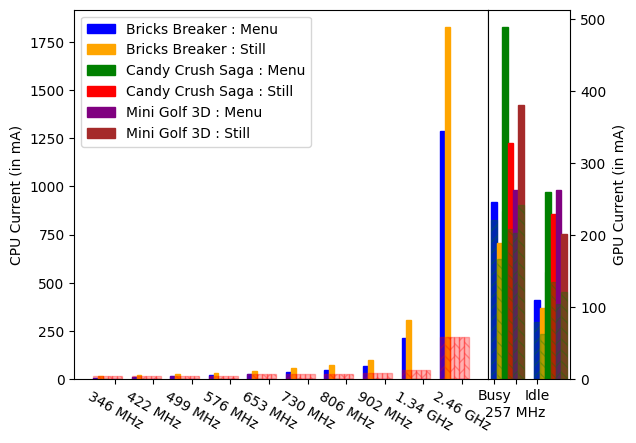
\includegraphics[width=\textwidth]{figures/002_Pixel2_1_nano_equations.png}
         \label{fig:number_parameters_vs_duration_100s_0}
     \end{subfigure}
    \begin{subfigure}[b]{0.32\textwidth}
         \centering
         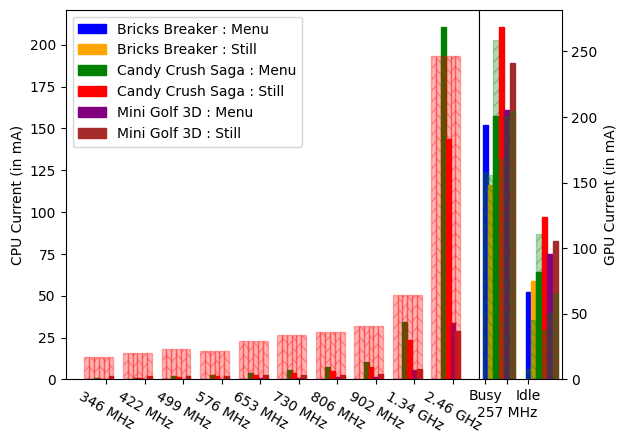
\includegraphics[width=\textwidth]{figures/003_MotoZ3_1_nano_equations.png}
         \label{fig:number_parameters_vs_duration_100s_100}
     \end{subfigure}
    \begin{subfigure}[b]{0.32\textwidth}
         \centering
         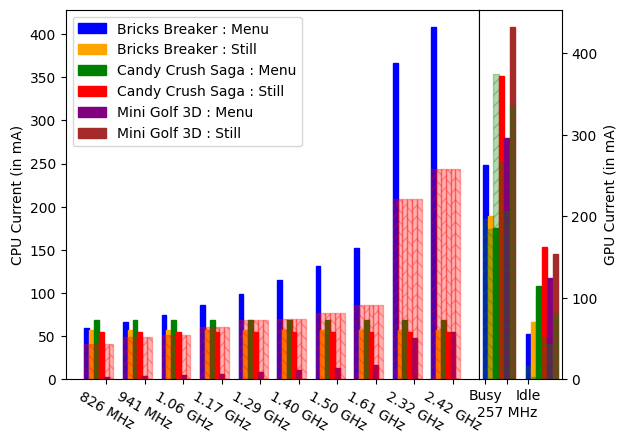
\includegraphics[width=\textwidth]{figures/004_Pixel4_1_nano_equations.png}
         \label{fig:number_parameters_vs_duration_100s_200}
     \end{subfigure}
     \hfill
     \centering
     \begin{subfigure}[b]{0.32\textwidth}
        \centering
    	{ \scriptsize
    	\begin{tabular}{ | l | c | c | c | c | c | c | }
    		\hline
    		     & \multicolumn{6}{ c|}{Error for each App Scenarios (in \%)}\\
    		\cline{2-7}
                    Model & \rot{B. Menu} & \rot{B. Still} & \rot{C. Menu} & \rot{C. Still} & \rot{M. Menu} & \rot{M. Still}  \\
    		\hline
                Fix. F. Const.       & 4.3 & 3.8 & 12 & 9.1 & 5.5 & 16 \\
                Classical            & 19 & 30 & 23 & 22 & 51 & 31 \\

    		\hline
    	\end{tabular}
    	}
	\caption{Pixel 2}
    \end{subfigure}
         \begin{subfigure}[b]{0.32\textwidth}
        \centering
    	{ \scriptsize
    	\begin{tabular}{ | l | c | c | c | c | c | c | }
    		\hline
    		     & \multicolumn{6}{ c|}{Error for each App Scenarios (in \%)}\\
    		\cline{2-7}
                    Model & \rot{B. Menu} & \rot{B. Still} & \rot{C. Menu} & \rot{C. Still} & \rot{M. Menu} & \rot{M. Still}  \\
    		\hline
                Fix. F. Const.       & 14 & 14 & 7.3 & 14 & 21 & 12 \\
                Classical            & 42 & 18 & 39 & 27 & 41 & 18 \\
    		\hline
    	\end{tabular}
    	}
	\caption{Moto Z3}
    \end{subfigure}
         \begin{subfigure}[b]{0.32\textwidth}
        \centering
    	{ \scriptsize
    	\begin{tabular}{ | l | c | c | c | c | c | c | }
    		\hline
    		     & \multicolumn{6}{ c|}{Error for each App Scenarios (in \%)}\\
    		\cline{2-7}
                    Model & \rot{B. Menu} & \rot{B. Still} & \rot{C. Menu} & \rot{C. Still} & \rot{M. Menu} & \rot{M. Still}  \\
    		\hline
                Fix. F. Const.       & 13 & 11 & 16 & 27 & 21 & 25 \\
                Classical            & 38 & 50 & 23 & 42 & 29 & 34 \\
    		\hline
    	\end{tabular}
    	}
	\caption{Pixel 4}
    \end{subfigure}
     \hfill
    \caption{Model parameters derived by nano-scale SPMD}
    \label{fig:nano}
    \vspace{-0.1in}
\end{figure*}

\paragraph{Findings}
Figure~\ref{fig:nano} shows the model parameters output of the Fixed Freq-constrained regression solver for the same six app scenarios.
We observe that the model parameters derived from nano-scale SPMD are again drastically different from the corresponding parameters derived from the classical model.
In particular, we see that for Moto Z3 for "Fix-Freq.-Constr. SPMD" for 16 equations
(1)The power models output by the solver have LSF error
between 6.4\% to 25.5\% for Pixel 2, between 4.3\% to 22.3\% for Moto Z3 and between 10.4\% to 33.9\% for Pixel 4
% (2) Depending upon The CPU model parameters are in the range of 0 mA ,0 mA,0-81 mA for Pixel 2 ,Moto Z3,Pixel 4 respectively.
(2)For  Pixel 4 out of 6 app scenarios CPU parameters are zero for 2 scenarios and less than 50\% of the classical model parameters for 3 scenarios .
Similarly, CPU parameters are zero for 2 scenarios and less than 50\%  of the classical model parameters for 4 scenarios for Moto Z3.
Whereas, CPU parameters are zero for Pixel 2.
% \comment{(2) In 3 out of the 12 scenarios marked in bold, the model parameters generated seem reasonable, \ie about 50\% of their counterparts in the classic model.}

\begin{table}[tp]
{\footnotesize
    \centering
    \caption{The rank and singular values for the set of equations for nano-scale "Fix-Freq.-Constr. SPMD" for Pixel 4  for 16 equation system of equation.
    (Top 4 singular values are shown.)
    }
    \vspace{-0.1in}
    \begin{tabular}{|c|p{9mm}|p{4.5mm}|p{4.5mm}|p{4.5mm}|p{4mm}|p{4mm}|p{4mm}|}
    \hline
        App & Scenario & Num. of Eqns. & Num. of Vars. & Rank &  \multicolumn{3}{c|}{Singular Values} \\
        \hline
        \multirow{2}{13mm}{Bricks Breaker} & Menu & 16 & 4 & 4 & 4.15  & 2.21  & 1.51 \\
         \cline{2-8}
         & Still & 16 & 4 & 4 & 4.16  & 1.65  & 1.11 \\
         \hline
        \multirow{2}{13mm}{Candy Crush Saga} & Menu & 16 & 4 & 4 & 4.34  & 3.00  & 2.28 \\
        \cline{2-8}
	     & Still & 16 & 4 & 4 & 4.86  & 2.69  & 0.87 \\
	     \hline
         \multirow{2}{13mm}{Mini Golf 3D} & Menu & 16 & 5 & 5 & 3.88  & 2.90  & 1.31 \\
         \cline{2-8}
         & Still & 16 & 5 & 5 & 4.14  & 3.10  & 2.18\\
         \hline

    \end{tabular}
    \label{tab:nano-rank_motoz3}
    \vspace{-0.1in}
}
\end{table}

Table~\ref{tab:nano-rank_motoz3} shows the systems of equations are full rank and have reasonable singular values for Moto Z3. 
%
% The rank is one off of the full rank due to the fact that CPU base power does not vary.
% To overcome this, we fixed the base power to the constant
% base power parameter value from the classical model, making the set of equations full rank.
% The model parameters output by the solver with this constraint 
% are shown in the rows labeled as "Fix-Freq-constr." in the same two tables.
% We observe that the solutions are still different from those in the classic
% model; in particular, the constraint simply shifted the high based power to high GPU Idle power.

\begin{table}[tp]
    \centering
    \caption{Equations for the 16.7 ms interval for Bricks Breaker Menu scenario on Moto Z3 for 16 equation set.}
    {\small
    \begin{tabular}{|c|c|c|c|c|}
        \hline
            Eqn & y(n) & \multicolumn{1}{c|}{CPU Utilization} & \multicolumn{2}{c|}{GPU Utilization} \\
%       \cline{2-4}
%            y(n)  & 422 MHz & \multicolumn{2}{c|}{257 MHz} \\
        \cline{4-5}
            & (mA) & \multicolumn{1}{c|}{} & Busy & Idle \\
        \hline
                 1 & 273.1 &  43\% &  100\% &    0\% \\
                 2 & 341.2 &   0\% &  100\% &    0\% \\
                 3 & 348.0 & 105\% &   78\% &   21\% \\
                 4 & 184.8 & 135\% &    0\% &  100\% \\
                 5 & 153.5 & 184\% &    0\% &  100\% \\
                 6 & 155.6 & 130\% &    0\% &  100\% \\
                 7 & 164.3 & 147\% &    0\% &  100\% \\
                 8 & 164.6 & 115\% &    0\% &  100\% \\
                 9 & 169.0 & 125\% &    0\% &  100\% \\
                10 & 166.7 & 127\% &    0\% &  100\% \\
                11 & 164.6 & 100\% &    0\% &  100\% \\
                12 & 166.8 & 124\% &    0\% &  100\% \\
                13 & 171.3 & 108\% &    0\% &  100\% \\
                14 & 166.2 & 137\% &    0\% &  100\% \\
                15 & 154.2 & 180\% &    0\% &  100\% \\
                16 & 165.7 & 124\% &    2\% &   97\% \\
        \hline
    \end{tabular}
    }
    \label{tab:equations_nano}
\end{table}

Finally, we looked into the individual equations to understand why 
Table~\ref{tab:equations_nano} shows the 16 equations for the 16.7 ms interval for Bricks Breaker Menu scenario for Moto Z3.
We make two observations.
(1) The equations fall into two groups, corresponding to the GPU Busy state and Idle state with equation corresponding to the transition. 
(2) Within each group, many equations contradict each other. For example,
the CPU utilization of Eqn.~14 are higher than 
those in Eqn.~13 yet the LHS energy values are the opposite. The same happens for group 2, \eg between Eqn.~1 and Eqn.~2. 
These numbers suggest that again the 16 equations not only did not add to the diversity, but actually
added noise to the equations making it hard for the solver to output meaningful model parameters. 

% \if 0
% We observe the some equation are not following the excepted trend.
% Like in $11^{th}$ and $12^{th}$ equations, the CPU utilization has gone up from 218\% to 328\% but the LHS fell from 160.00 mA to 153.20 mA.
% In nano-scale the measurement noise is very high due to it's short duration per equations.
% The noise gets averaged out over longer duration in macro-scale and micro-scale equations.
% The noise becomes the prominent factor and the equation can't capture the subtle trends.
% This makes the solution to be unexpected
% like the CPU parameter for "Fix-Freq-Constr." SPMD to be 0.00 mA instead of the expected 13.77 mA.
% (2) Using the LHS of the equations, the equations can be divided broadly into two camps.
% One set when GPU is in Active-busy and other when the GPU in Active-idle.
% This shows that we are still falling short of truly diverse set of more than 2 equations.
% This makes the set of equation still under-determined when trying to solve for 3 variables in "Fix-Freq-Constr." SPMD.
% \fi

% This is because the 16 equations generated are not independent on each other and could not precisely identify the subtle changes in CPU usages. Let's consider the Boat Racing Intro scenario, the CPU coefficient as expected is 13.77 mA. We observe in the equation that the swing of CPU power as predicted by the classical model is not more than 30 mA. Due to measurements noise, these changes in CPU power couldn't be deciphered as noise or signal, giving us unexpected results. Furthermore, GPU coefficients are sometimes a order higher than the CPU coefficient making the solver giving prejudicial solutions.
% This is because the GPU Active-busy and Active-idle states are not independent because the sum of there duration is always constant as 16.7 ms.
% \comment{this does not make sense. think x+2y = 3, 2x+y=4 are x and y  independenty?}

% \comment{
% Furthermore, at nano-scale, \ie 1ms regime, the noise in the measurement of power monitor readings, alignment error and uncompensated power spikes due to other components
% becomes significant.
% This introduces error to the equations which affects the solution generated by the regression solver. 
% }

% \comment{The variable for base current is always present  and do not vary, making it rank deficient. ??? what does this mean? }

%% 6. Conclusion
The above experiments and analysis suggest that 
nano-scale SMPD, \ie creating equations at 1ms granularity, is also impractical to derive meaningful model parameters.
\section{Related Work}
\label{sec:related}

The large amount of prior work on power modeling can be categorized along three dimensions: 
model type, using external power monitor or self-metering, and model derivation process.

\paragraph{Utilization-based vs. FSM-based power models} 
The large number of power models for different components of 
smartphones can be grouped into two categories
based on the way it captures two different types of phone component power draw behaviors. 
The first category of power models known as utilization-based models
(\eg \cite{shye2009into,zhang2010accurate,hotpowermulticore}) 
captures the synchronous power draw behavior of  components ; where
a hardware component enters a certain power state and draws power for the duration
when it is actively used in that state, \eg the CPU running at 2 GHz 
% and change of utilization is what triggers the power state change of that component. 
Consequently, these models use the utilization of a hardware component as an input to the power models.
% ``trigger'' in modeling power states and state transitions.  

% Such models thus do not capture power behavior of
% modern wireless components that do not lead to active utilization such
% as the promotion and tail power behavior of 3G and
% LTE~\cite{rrc:imc2010,4glte}, and thus can incur high modeling error.

The second category known as non-utilization-based power models captures the asynchronous power 
draw behavior of hardware components where an app’s usage of a phone component
triggers that component to enter some power state and continues even beyond the duration of the app usage.
Non-utilization-based models capture such power behavior using finite state machines (FSMs),
\eg \cite{arunabimc09,energybasedRA,aro,whatsup:mobicom12,pathak:eurosys12,ding:sigmetrics13}
for WiFi, 3G and~\cite{4glte} for 4G/LTE. 
To derive such models, the built-in state machine of such hardware components, \eg the RRC states and
transitions in the LTE radio, is reverse-engineered and represented in an FSM
annotated with app utilization, \eg either packet-level traces~\cite{rrc:imc2010,4glte} or
networking system calls~\cite{pathak:eurosys12}, as the triggers for the state transitions.

\paragraph{Using external power monitor vs. self-metering}
Deriving the power models of a mobile device 
requires ground-truth power draw measurement, whether it is for one component as in case of TPMD or for several components as a whole as in case of SPMD. This can be done using an external power monitor such as Monsoon~\cite{powermonitor} or
using energy information from the built-in battery interface. 

PowerBooter~\cite{powerbooter:2010} proposed to use battery State-of-Charge (SoD) readings to infer the average power draw has a very long generation time. 
%
Sesame~\cite{sesame:2011} uses drop in the battery capacity  during a sampling interval  to infer average power draw but it shows a high error at 0.1 Hz.
% 
V-edge~\cite{vedge:2013} exploits the correlation between change in current and voltage  
to extrapolate  power draw (relative to a baseline) using only voltage readings.  
DevScope~\cite{devscope:2012} studies the approach towards overcoming the coarse granularity of current sensor readings to derive power models for one single component at a time.  
%
Since Android 6, Android phones provided interfaces for power or energy readings which however come
with limited accuracy as discussed in \S\ref{subsec:modelling_sensor}.



\paragraph{TPMD vs. SPMD}
The third dimension of power modeling is whether to derive the model of one phone component state at a time by isolating the measured power for each of the component state as in case of TPMD, or 
to derive the model for all the component states by solving a system of equations as in case of SPMD, as already discussed in \S\ref{subsec:back}.
\section{Conclusion}
\label{sec:conc}

In this paper, we performed an in-depth study of the feasibility of self-constructive per-component power model
derivation (SPMD) on modern smartphones. Using two representative phones,
we identified the equation diversity as the primary challenge of SPMD
and explored diverse time-scales in trying to create equations that exhibit high diversity.  
Our experiments and analysis have shown that it is extremely difficult to create equations with sufficient diversity for the regression solver to generate meaningful per-component power model parameters. 
Our verification work debunked a myth about the applicability of SPMD at the per-component level.

\bibliographystyle{abbrv}
% \bibliography{ref}
\bibliography{mobile}

% \section*{Appendix: Results for Nexus 6 }
%%%%%%%%%%%%%%%% Micro scale

The GPU in Nexus 6 can run at 5 different frequencies and three power states; Active, Init and Nap. Init corresponds to Aware and Nap corresponds to Slumber of Moto Z3.

Since Nexus 6 has a weaker GPU, Boat Racing ran with average GPU utilization close to 100\%
% 95.6\%
and barely entering the GPU Idle state.
Thus we used Bricks Breaker and Candy Crush Saga for Nexus 6 experiments 
which had an average GPU utilization of 77.01\% and 61.82\% respectively.

For Nexus 6, the game apps run with high GPU utilization causing the phone temperature to increase. 
To prevent the phone from switching off cores during app runs due to thermal throttling,
we performed SPMD modeling on Nexus 6 with only 2 CPU cores turned on.


\paragraph{Freq-constrained SPMD} 
For Nexus 6, when we model the core power as a polynomial of frequency, 
we found the fitted exponent $n$ for 1, 2 and 4 cores to be {1.85, 2.04 and 2.25, respectively}. 
Therefore we model the Nexus 6 core as a second-order polynomial of CPU frequency.
\comment{which exponent?}

\subsection*{A1. GPU Power Model is App Dependent for Nexus 6}
\begin{table*}[tp]
{\footnotesize
    \centering
    \caption{Nexus 6 GPU power model (active-busy and active-idle power per frequency) with the CPU fixed at 1.037 GHz.}
    \vspace{-0.1in}
    \begin{tabular}{|p{15mm}|p{9mm}|c|c|c|c|c|c|c|c|c|c|}
    \hline
    App & Scenario & \multicolumn{10}{c|}{GPU Frequency} \\
    \cline{3-12}
     &  & \multicolumn{2}{c|}{240 MHz} & \multicolumn{2}{c|}{300 MHz} & \multicolumn{2}{c|}{389 MHz} & \multicolumn{2}{c|}{500 MHz} & \multicolumn{2}{c|}{600 MHz} \\
     \cline{3-12}
     & & Busy & Idle & Busy & Idle & Busy & Idle & Busy & Idle & Busy & Idle \\
    \hline
      \multirow{2}{15mm}{Candy Crush Saga}  & Intro & 387.4 & 378.9 & 520.3 & 390.9 & 640.0 & 432.9 & 880.3 & 408.3 & 1387.2 & 378.9 \\
      \cline{2-12}
         & Tutorial & 625.4 & 747.0 & 375.0 & 908.2 & 790.8 & 523.4 & 1022.0 & 493.4 & 1211.4 & 602.4 \\
         \hline
        \multirow{2}{13mm}{Bricks Breaker}  & Into & 411.2 & 261.0 & 498.2 & 193.6 & 596.9 & 254.7 & 817.2 & 298.7 & 1181.3 & 410.7 \\
        \cline{2-12}
         & Still & 387.7 & 348.6 & 635.5 & 373.3 & 553.9 & 260.5 & 757.4 & 292.5 & 994.2 & 420.7 \\
         \hline
    \end{tabular}
    \label{tab:gpumodel_nexus6}
    \vspace{-0.1in}
    }
\end{table*}

\subsection*{A2. Model Parameters by Macro-scale SPMD for Nexus 6}
\begin{table*}[tp]
\caption{Model parameters derived by macro-scale SPMD for Nexus 6. The classic models for GPU are from Table~\ref{tab:gpumodel_nexus6}. (Only model parameters for 3 CPU frequencies with highest utilization are shown due to space constraint.)}
\vspace{-0.1in}
{\footnotesize
    \begin{tabular}{|c|c|c|c|c|c|c|c|c|c|}
    \hline
        Model & Base & \multicolumn{3}{c|}{CPU Frequency} & \multicolumn{4}{c|}{GPU Frequency} & Error \\
    \cline{3-9}
        & & \multicolumn{3}{c|}{} & Busy & Idle & Busy & Idle & (\%) \\
    \hline
    \multicolumn{10}{|c|}{\bf Candy Crush Saga Intro Scenario} \\
        \hline
        &  & 730 MHz & 1.27 GHz & 1.57 GHz & \multicolumn{2}{c|}{240 MHz} & \multicolumn{2}{c|}{300 MHz} & \\
        \hline
        Unconstr. SPMD & -134.6 & 3.46 & 81.70 & 232.8 & 545.5 & 325.5 & 933.9 & 150.5 & 0.92 \\
        Constr. SPMD & 0.00 & 39.52 & 111.3 & 228.3 & 544.8 & 5.79 & 698.9 & 5.79 & 1.17 \\
        Freq-Constr. SPMD& 3.62 & 46.73 & 141.0 & 217.6 & 524.7 & 0.00 & 819.8 & 0.00 & 1.55 \\
        \hline
        Classical & 20.16 & 53.35 & 138.0 & 186.5 & 387.4 & 378.9 & 520.3 & 390.9 & 43.50 \\
        \hline

    \multicolumn{10}{|c|}{\bf Candy Crush Saga Tutorial Scenario} \\
        \hline
        &  & 730 MHz & 960 MHz & 1.27 GHz & \multicolumn{2}{c|}{240 MHz} & \multicolumn{2}{c|}{300 MHz} & \\
        \hline
        Unconstr. SPMD & 17209948.0 & 339.8 & 550.3 & 246.5 & -17209018.0 & -17209618.0 & -17209370.3 & -17209132.4 & 4.76 \\
        Constr. SPMD & 258.0 & 53.48 & 53.48 & 53.48 & 143.0 & 103.8 & 168.3 & 129.2 & 4.97 \\
        Freq-Constr. SPMD& 517.6 & 0.00 & 0.00 & 0.00 & 23.18 & 23.18 & 36.22 & 36.22 & 4.96 \\
        \hline
        Classical & 20.16 & 53.35 & 107.1 & 138.0 & 625.4 & 747.0 & 375.0 & 908.2 & 158.4 \\
        \hline

        
    \multicolumn{10}{|c|}{\bf Break Breakers Into Scenario} \\
        \hline
        &  & 960 MHz & 1.27 GHz & 1.57 GHz & \multicolumn{2}{c|}{240 MHz} & \multicolumn{2}{c|}{300 MHz} & \\
        \hline
        Unconstr. SPMD & -57.12 & -607.1 & -55.5 & -1444.0 & 356.4 & 937.5 & 469.6 & 774.4 & 2.63 \\
        Constr. SPMD & 358.2 & 15.69 & 15.69 & 15.69 & 0.36 & 0.36 & 75.24 & 0.36 & 2.78 \\
        Freq-Constr. SPMD& 274.9 & 0.00 & 0.00 & 0.00 & 90.44 & 90.44 & 141.3 & 141.3 & 2.81 \\
        \hline
        Classical & 20.16 & 107.1 & 138.0 & 186.5 & 411.2 & 261.0 & 498.2 & 193.6 & 22.66 \\
        \hline

    \multicolumn{10}{|c|}{\bf Break Breakers Still Scenario} \\
        \hline
        &  & 1.04 GHz & 1.27 GHz & 1.57 GHz & \multicolumn{2}{c|}{240 MHz} & \multicolumn{2}{c|}{-} & \\
       \hline
        Unconstr. SPMD & 366.2 & 216.2 & 201.0 & 236.5 & -0.13 & -23.17 & - & - & 0.55 \\
        Constr. SPMD & 70.35 & 161.5 & 161.5 & 282.9 & 263.1 & 212.6 & - & - & 0.63 \\
        Freq-Constr. SPMD& 222.3 & 101.6 & 151.8 & 234.3 & 77.45 & 61.03 & - & - & 0.72 \\
        \hline
        Classical & 20.16 & 114.4 & 138.0 & 186.5 & 387.7 & 348.6 & - & - & 34.65 \\
        \hline

\end{tabular}
}
\label{tab:nexus6macro}
\vspace{-0.1in}
\end{table*}

\begin{table*}[tp]
% \questionaj{Also add rank of freq-constrained case}
{\small
    \centering
    \caption{The rank and singular values for the set of equations for macro-scale SPMD for Nexus 6.}
    \vspace{-0.1in}
    \begin{tabular}{|c|c|c|c|c|c|c|c|c|c|c|c|c|c|c|c|}
    \hline
        App & Scenario & \# of Eqns. & \# of Vars. & Rank &  \multicolumn{11}{c|}{Singular Values} \\
        \hline
        \multirow{2}{15mm}{Candy Crush Saga} & Into & 100 & 17 & 16 & 13.00  & 1.86  & 0.75  & 0.62  & 0.59  & 0.50  & 0.49  & 0.44  & 0.37  & 0.32  & 0.30 \\
        \cline{2-16}
	     & Tutorial &  100 & 18 & 18 & 28.76  & 1.74  & 1.23  & 0.69  & 0.47  & 0.32  & 0.28  & 0.24  & 0.22  & 0.20  & 0.16\\
	     \hline
	     \multirow{2}{15mm}{Bricks Breaker} & Into & 100 & 15 & 13 & 13.98  & 1.89  & 0.65  & 0.51  & 0.45  & 0.29  & 0.17  & 0.12  & 0.08  & 0.04  & 0.04 \\
         \cline{2-16}
         & Still & 100 & 15 & 14 & 14.26  & 1.06  & 0.48  & 0.35  & 0.30  & 0.22  & 0.18  & 0.11  & 0.06  & 0.05  & 0.05 \\
         \hline
    \end{tabular}
    \label{tab:macro_singularvalues_nexus6}
    \vspace{-0.1in}
}
\end{table*}

\subsection*{A3. Model Parameters by Micro-scale SPMD for Nexus 6}
The solution for Micro-scale SPMD for Nexus 6 is shown in Table~\ref{tab:nexus6micro}.
\begin{table*}[tp]
\caption{Model parameters derived by micro-scale SPMD For Nexus 6.}
\vspace{-0.1in}
{\footnotesize
    \begin{tabular}{|c|c|c|c|c|p{5.4mm}|}
    \hline
        Model & Base & \multicolumn{1}{c|}{CPU Frequency} & \multicolumn{2}{c|}{GPU Frequency} & Error \\
    \cline{3-5}
        & & \multicolumn{1}{c|}{} & Busy & Idle & (in\%) \\
    \hline
    \multicolumn{6}{|c|}{\textbf{Candy Crush Saga Intro Scenario}} \\
        \hline
        &  & 1.19 GHz & \multicolumn{2}{c|}{240 MHz} & \\
        \hline
        % Unconstrained & 200.45 & -3.53 & 446.33 & 426.98 & 0.16 \\
        % Constrained & 623.96 & 0.00 & 21.54 & 0.00 & 0.15 \\
        Freq-Constr. & 419.2 & 0.00 & 226.3 & 204.8 & 0.15 \\
        \hline
        Classical & 20.16 & 130.5 & 387.4 & 378.9 & 23.31 \\
        \hline

    \multicolumn{6}{|c|}{\textbf{Candy Crush Saga Tutorial Scenario}} \\
        \hline
        &  & 422 MHz & \multicolumn{2}{c|}{240 MHz} & \\
        \hline
        % Unconstrained & 98.24 & -60.52 & 462.65 & 352.91 & 13.22 \\
        % Constrained & 45.50 & 0.00 & 467.24 & 367.76 & 14.64 \\
        Freq-Constr. & 413.3 & 0.00 & 99.48 & 0.00 & 14.64 \\
        \hline
        Classical & 20.16 & 32.17 & 625.4 & 747.0 & 64.32 \\
        \hline

    \multicolumn{6}{|c|}{\textbf{Brick Breakers Intro Scenario}} \\
        \hline
        &  & 422 MHz & \multicolumn{2}{c|}{240 MHz} & \\
        \hline
        % Unconstrained & 579.53 & 56.86 & -291.08 & -377.19 & 3.52 \\
        % Constrained & 0.06 & 56.86 & 288.39 & 202.28 & 3.52 \\
        Freq-Constr. & 145.2 & 56.86 & 143.3 & 57.19 & 3.52 \\
        \hline
        Classical & 20.16 & 32.17 & 411.2 & 261.0 & 25.58 \\
        \hline

    \multicolumn{6}{|c|}{\textbf{Brick Breakers Still Scenario}} \\
        \hline
        &  & 422 MHz & \multicolumn{2}{c|}{240 MHz} & \\
        \hline
        % Unconstrained & -125.55 & 8.21 & 428.48 & 426.29 & 3.53 \\
        % Constrained & 200.87 & 8.21 & 102.07 & 99.87 & 3.53 \\
        Freq-Constr. & 300.7 & 8.21 & 2.20 & 0.00 & 3.53 \\
        \hline
        Classical & 20.16 & 32.17 & 387.7 & 348.6 & 37.10 \\
        \hline

\end{tabular}
}
\label{tab:nexus6micro}
\vspace{-0.1in}
\end{table*}

\begin{table*}[tp]
{\footnotesize
    \centering
    \caption{The rank and singular values for the set of equations for micro-scale SPMD for Nexus 6.}
    \vspace{-0.1in}
    \begin{tabular}{|c|p{9mm}|p{4.5mm}|p{4.5mm}|p{4mm}|p{4mm}|p{4mm}|p{4mm}|p{4mm}|}
    \hline
        App & Scenario & Num. of Eqns. & Num. of Vars. & Rank &  \multicolumn{4}{c|}{Singular Values} \\
        \hline
        \multirow{2}{13mm}{Candy Crush Saga} & Into & 4 & 4 & 3 & 2.77  & 1.30  & 0.10  & 0.00 \\
        \cline{2-9}
	     & Tutorial & 4 & 4 & 3 & 2.84  & 1.41  & 0.41  & 0.00 \\
	     \hline
         \multirow{2}{13mm}{Bricks Breaker} & Into & 4 & 4 & 3 & 3.39  & 1.42  & 0.05  & 0.00 \\
         \cline{2-9}
         & Still & 4 & 4 & 3 & 3.45  & 1.40  & 0.24  & 0.00 \\
         \hline
    \end{tabular}
    \label{tab:micro-rank_nexus6}
    \vspace{-0.1in}
}
\end{table*}

\subsection*{A4. Model Parameters by Nano-scale SPMD for Nexus 6}
\begin{table*}[tp]
\caption{Model parameters derived by Nano-scale SPMD for Nexus 6.}
\vspace{-0.1in}
{\footnotesize
\begin{tabular}{|c|c|c|c|c|p{5.4mm}|}
    \hline
        Model & Base & \multicolumn{1}{c|}{CPU Frequency} & \multicolumn{2}{c|}{GPU Frequency} & Error \\
     \cline{3-5}
            & & \multicolumn{1}{c|}{} & Busy & Idle & (in\%) \\
    \hline
    \multicolumn{6}{|c|}{\textbf{Candy Crush Saga Intro Scenario}} \\
        \hline
        &  & 1.50 GHz & \multicolumn{2}{c|}{240 MHz} & \\
        \hline
        % Unconstrained & 428.97 & -105.79 & 59.79 & -23.67 & 14.14 \\
        % Constrained & 1.65 & 0.00 & 365.91 & 365.91 & 19.61 \\
        Freq-Constr. & 367.6 & 0.00 & 0.00 & 0.00 & 19.61 \\
        Fix-Freq-Constr. & 20.16 & 0.00 & 347.4 & 347.4 & 19.61 \\
        \hline
        Classical & 20.16 & 166.3 & 387.4 & 378.9 & 62.93 \\
        \hline

    \multicolumn{6}{|c|}{\textbf{Candy Crush Saga Tutorial Scenario}} \\
        \hline
        &  & 1.96 GHz & \multicolumn{2}{c|}{240 MHz} & \\
        \hline
        % Unconstrained & -1915.95 & 746.61 & 976.22 & 741.52 & 15.27 \\
        % Constrained & 0.00 & 252.18 & 58.73 & 0.00 & 17.27 \\
        Freq-Constr. & 0.00 & 252.2 & 58.73 & 0.00 & 17.27 \\
        Fix-Freq-Constr. & 20.16 & 243.7 & 55.70 & 0.00 & 17.32 \\
        \hline
        Classical & 20.16 & 245.5 & 625.4 & 747.0 & 111.5 \\
        \hline


    \multicolumn{6}{|c|}{\textbf{Bricks Breaker Intro Scenario}} \\
        \hline
        &  & 422 MHz & \multicolumn{2}{c|}{240 MHz} & \\
        \hline
        % Unconstrained & 446.23 & -21.18 & -72.12 & -132.84 & 36.29 \\
        % Constrained & 284.61 & 0.00 & 69.00 & 0.56 & 36.12 \\
        Freq-Constr. & 78.74 & 0.00 & 274.9 & 206.4 & 36.12 \\
        Fix-Freq-Constr. & 20.16 & 0.00 & 333.5 & 265.0 & 36.12 \\
        \hline
        Classical & 20.16 & 32.17 & 411.2 & 261.0 & 49.17 \\
        \hline

    \multicolumn{6}{|c|}{\textbf{Bricks Breaker Still Scenario}} \\
        \hline
        &  & 422 MHz & \multicolumn{2}{c|}{240 MHz} & \\
        \hline
        % Unconstrained & -216.04 & 81.08 & 430.76 & 423.06 & 26.90 \\
        % Constrained & 204.36 & 81.08 & 10.36 & 2.67 & 26.90 \\
        Freq-Constr. & 169.4 & 81.08 & 45.28 & 37.59 & 26.90 \\
        Fix-Freq-Constr. & 20.16 & 81.08 & 194.6 & 186.9 & 26.90 \\
        \hline
        Classical & 20.16 & 32.17 & 387.7 & 348.6 & 57.65 \\
        \hline
\end{tabular}
\label{tab:nano_nexus6}
}
\vspace{-0.1in}
\end{table*}

\begin{table*}[tp]
{\footnotesize
    \centering
    \caption{The rank and singular values for the set of equations for nano-scale SPMD for Nexus 6.}
    \vspace{-0.1in}
    \begin{tabular}{|c|p{9mm}|p{4.5mm}|p{4.5mm}|p{4mm}|p{4mm}|p{4mm}|p{4mm}|p{4mm}|}
    \hline
        App & Scenario & Num. of Eqns. & Num. of Vars. & Rank &  \multicolumn{4}{c|}{Singular Values} \\
        \hline
        \multirow{2}{13mm}{Candy Crush Saga} & Into & 16 & 4 & 3 & 6.00  & 2.83  & 1.02  & 0.00 \\
        \cline{2-9}
	     & Tutorial & 16 & 4 & 3 & 9.83  & 1.18  & 0.13  & 0.00 \\
	     \hline
         \multirow{2}{13mm}{Bricks Breaker} & Into & 16 & 4 & 3 & 6.70  & 2.78  & 1.01  & 0.00 \\
         \cline{2-9}
         & Still & 16 & 4 & 3 & 6.88  & 2.21  & 1.00  & 0.00 \\
         \hline
    \end{tabular}
    \label{tab:nano-rank_nexus6}
    \vspace{-0.1in}
}
\end{table*}



















\if 0
\subsection*{A.1 Results for Per-Component SPMD with Power Monitor:Micro-Scale}
Table~\ref{tab:micro} and table~\ref{tab:nexus6micro} are the solution estimated from SPMD
for Moto Z3 and Nexus 6 respectively from macro-scale.

\begin{table}[]
\caption{Model parameters derived by Micro-scale SPMD for Moto Z3}
\vspace{-0.1in}
{\footnotesize
    \begin{tabular}{|c|c|c|c|c|p{5.4mm}|}
    \hline
    \multicolumn{6}{|c|}{Boat Racing Into Scenario} \\
        \hline
         Model & Base & \multicolumn{1}{c|}{CPU Frequency} & \multicolumn{2}{c|}{GPU Frequency} & Error \\
        \cline{3-5}
        &  & 346 MHz & \multicolumn{2}{c|}{342 MHz} & (in\%)\\
        \cline{3-5}
                & & \multicolumn{1}{|c|}{} & Busy & Idle & \\
        \hline
        Unconstrained & -499.67 & 10.86 & 700.28 & 738.70 & 3.89 \\
        Constrained & 8.46 & 43.81 & 126.02 & 126.02 & 6.02 \\
        Freq-Constr. & 93.31 & 43.81 & 41.17 & 41.17 & 6.02 \\
        \hline
        Classical & 27.86 & 13.77 & 253.74 & 67.25 & 42.32 \\
        \hline

    \multicolumn{6}{|c|}{Boat Racing Still Scenario} \\
        \hline
        Model & Base & \multicolumn{1}{c|}{CPU Frequency} & \multicolumn{2}{c|}{GPU Frequency} & Error \\
        \cline{3-5}
        &  & 499 MHz & \multicolumn{2}{c|}{342 MHz} & (in\%) \\
        \cline{3-5}
                & & \multicolumn{1}{|c|}{} & Busy & Idle & \\
        \hline
        Unconstrained & 800.65 & 10.33 & -470.88 & -644.35 & 0.06 \\
        Constrained & 0.00 & 10.33 & 329.77 & 156.30 & 0.06 \\
        Freq-Constr. & 152.98 & 10.33 & 176.80 & 3.32 & 0.06 \\
        \hline
        Classical & 27.86 & 18.65 & 357.96 & 57.00 & 25.19 \\
        \hline


    \multicolumn{6}{|c|}{Candy Crush Saga Intro Scenario} \\
        \hline
        Model & Base & \multicolumn{1}{c|}{CPU Frequency} & \multicolumn{2}{c|}{GPU Frequency} & Error \\
        \cline{3-5}
        &  & 422 MHz & \multicolumn{2}{c|}{257 MHz} & (in\%)\\
        \cline{3-5}
                & & \multicolumn{1}{|c|}{} & Busy & Idle & \\
        \hline
        Unconstrained & 208.63 & -9.86 & 46.81 & -70.63 & 1.60 \\
        Constrained & 0.16 & 0.00 & 243.92 & 124.38 & 2.06 \\
        Freq-Constr. & 101.50 & 0.00 & 142.59 & 23.04 & 2.06 \\
        \hline
        Classical & 27.86 & 16.01 & 227.99 & 83.88 & 9.98 \\
        \hline
        
    \multicolumn{6}{|c|}{Candy Crush Saga Tutorial Scenario} \\
        \hline
        Model & Base & \multicolumn{1}{c|}{CPU Frequency} & \multicolumn{2}{c|}{GPU Frequency} & Error \\
        \cline{3-5}
        &  & 576 MHz & \multicolumn{2}{c|}{257 MHz} & (in\%) \\
        \cline{3-5}
                & & \multicolumn{1}{|c|}{} & Busy & Idle & \\
        \hline
        Unconstrained & 535.72 & 18.00 & -297.80 & -422.77 & 0.82 \\
        Constrained & 85.15 & 18.00 & 152.78 & 27.80 & 0.82 \\
        Freq-Constr. & 96.49 & 18.00 & 141.44 & 16.47 & 0.82 \\
        \hline
        Classical & 27.86 & 20.96 & 226.29 & 92.85 & 8.05 \\
        \hline
\end{tabular}
}
\label{tab:micro_a}
\vspace{-0.1in}
\end{table}

\begin{table}[]
\caption{Model parameters derived by Micro-scale SPMD For Nexus6}
\vspace{-0.1in}
{\footnotesize
    \begin{tabular}{|c|c|c|c|c|p{5.4mm}|}
    \hline
    \multicolumn{6}{|c|}{Candy Crush Saga Intro Scenario} \\
        \hline
        Model & Base & \multicolumn{1}{c|}{CPU Frequency} & \multicolumn{2}{c|}{GPU Frequency} & Error \\
        \cline{3-5}
        &  & 1.19 GHz & \multicolumn{2}{c|}{240 MHz} & (in\%)\\
        \cline{3-5}
                & & \multicolumn{1}{|c|}{} & Busy & Idle & \\
        \hline
        Unconstrained & 200.45 & -3.53 & 446.33 & 426.98 & 0.16 \\
        Constrained & 623.96 & 0.00 & 21.54 & 0.00 & 0.15 \\
        Freq-Constr. & 419.18 & 0.00 & 226.32 & 204.78 & 0.15 \\
        \hline
        Classical & 20.16 & 130.53 & 387.41 & 378.94 & 23.31 \\
        \hline

    \multicolumn{6}{|c|}{Candy Crush Saga Tutorial Scenario} \\
        \hline
        Model & Base & \multicolumn{1}{c|}{CPU Frequency} & \multicolumn{2}{c|}{GPU Frequency} & Error \\
        \cline{3-5}
        &  & 422 MHz & \multicolumn{2}{c|}{240 MHz} & (in\%)\\
        \cline{3-5}
                & & \multicolumn{1}{|c|}{} & Busy & Idle & \\
        \hline
        Unconstrained & 98.24 & -60.52 & 462.65 & 352.91 & 13.22 \\
        Constrained & 45.50 & 0.00 & 467.24 & 367.76 & 14.64 \\
        Freq-Constr. & 413.27 & 0.00 & 99.48 & 0.00 & 14.64 \\
        \hline
        Classical & 20.16 & 32.17 & 625.40 & 747.00 & 64.32 \\
        \hline

    \multicolumn{6}{|c|}{Brick Breakers Intro Scenario} \\
        \hline
        Model & Base & \multicolumn{1}{c|}{CPU Frequency} & \multicolumn{2}{c|}{GPU Frequency} & Error \\
        \cline{3-5}
        &  & 422 MHz & \multicolumn{2}{c|}{240 MHz} & (in\%) \\
        \cline{3-5}
                & & \multicolumn{1}{|c|}{} & Busy & Idle & \\
        \hline
        Unconstrained & 579.53 & 56.86 & -291.08 & -377.19 & 3.52 \\
        Constrained & 0.06 & 56.86 & 288.39 & 202.28 & 3.52 \\
        Freq-Constr. & 145.15 & 56.86 & 143.30 & 57.19 & 3.52 \\
        \hline
        Classical & 20.16 & 32.17 & 411.24 & 261.02 & 25.58 \\
        \hline

    \multicolumn{6}{|c|}{Brick Breakers Still Scenario} \\
        \hline
        Model & Base & \multicolumn{1}{c|}{CPU Frequency} & \multicolumn{2}{c|}{GPU Frequency} & Error \\
        \cline{3-5}
        &  & 422 MHz & \multicolumn{2}{c|}{240 MHz} & (in\%) \\
        \cline{3-5}
                & & \multicolumn{1}{|c|}{} & Busy & Idle & \\
        \hline
        Unconstrained & -125.55 & 8.21 & 428.48 & 426.29 & 3.53 \\
        Constrained & 200.87 & 8.21 & 102.07 & 99.87 & 3.53 \\
        Freq-Constr. & 300.74 & 8.21 & 2.20 & 0.00 & 3.53 \\
        \hline
        Classical & 20.16 & 32.17 & 387.74 & 348.64 & 37.10 \\
        \hline

\end{tabular}
}
\label{tab:nexus6micro_a}
\vspace{-0.1in}
\end{table}

%%%%%%%%%%%%%%%%%%%%%% Nano Scale
\subsection*{A2. Results for Per-Component SPMD with Power Monitor:Nano-Scale}

Table~\ref{tab:nano} and table~\ref{tab:nexus6nano} are the solution estimated from SPMD
for Moto Z3 and Nexus 6 respectively from nano-scale.

\begin{table}[]
\caption{Model parameters derived by Nano-scale SPMD for Moto Z3}
\vspace{-0.1in}
{\footnotesize
\begin{tabular}{|c|c|c|c|c|c|}
    \hline
%    \multicolumn{2}{|c|}{CPU Model} & \multicolumn{2}{c|}{GPU Model} & & \\
%    \hline
    % Model & Base & CPU Frequency & \multicolumn{2}{c|}{GPU Frequency} & Error (in\%) \\
    % \cline{3-5}
    %  & & 806.4 MHz &  \multicolumn{2}{c|}{257 MHz} & \\
    % \cline{3-5}
    %         & & \multicolumn{1}{|c|}{} & Busy & Idle & \\
    % \hline
    \multicolumn{6}{|c|}{Boat Racing Into Scenario} \\
        \hline
        Model & Base & \multicolumn{1}{c|}{CPU Frequency} & \multicolumn{2}{c|}{GPU Frequency} & Error \\
        \cline{3-5}
        &  & 422 MHz & \multicolumn{2}{c|}{342 MHz} & (in\%) \\
        \cline{3-5}
                & & \multicolumn{1}{|c|}{} & Busy & Idle & \\
        \hline
        Unconstrained & 221.75 & 20.97 & -35.24 & -24.77 & 17.57 \\
        Constrained & 0.17 & 22.26 & 186.79 & 186.79 & 18.15 \\
        Freq-Constr. & 174.63 & 22.26 & 12.32 & 12.32 & 18.15 \\
        Fix-Freq-Constr. & 27.86 & 22.26 & 159.10 & 159.10 & 18.15 \\
        \hline
        Classical & 27.86 & 16.01 & 253.74 & 67.25 & 45.95 \\
        \hline

    \multicolumn{6}{|c|}{Boat Racing Still Scenario} \\
        \hline
        Model & Base & \multicolumn{1}{c|}{CPU Frequency} & \multicolumn{2}{c|}{GPU Frequency} & Error \\
        \cline{3-5}
        &  & 1.06 GHz & \multicolumn{2}{c|}{342 MHz} & (in\%) \\
        \cline{3-5}
                & & \multicolumn{1}{|c|}{} & Busy & Idle & \\
        \hline
        Unconstrained & -145.33 & -14.83 & 543.17 & 329.22 & 7.84 \\
        Constrained & 167.21 & 0.00 & 209.02 & 0.72 & 8.82 \\
        Freq-Constr. & 5.25 & 0.00 & 370.98 & 162.69 & 8.82 \\
        Fix-Freq-Constr. & 27.86 & 0.00 & 348.38 & 140.08 & 8.82 \\
        \hline
        Classical & 27.86 & 36.62 & 357.96 & 57.00 & 21.78 \\
        \hline

    \multicolumn{6}{|c|}{Candy Crush Saga Intro Scenario} \\
        \hline
        Model & Base & \multicolumn{1}{c|}{CPU Frequency} & \multicolumn{2}{c|}{GPU Frequency} & Error \\
        \cline{3-5}
        &  & 1.57 GHz & \multicolumn{2}{c|}{257 MHz} & (in\%) \\
        \cline{3-5}
                & & \multicolumn{1}{|c|}{} & Busy & Idle & \\
        \hline
        Unconstrained & -48.45 & 21.13 & 142.57 & 230.79 & 15.98 \\
        Constrained & 0.12 & 42.02 & 119.60 & 119.60 & 26.94 \\
        Freq-Constr. & 115.46 & 42.02 & 4.26 & 4.26 & 26.94 \\
        Fix-Freq-Constr. & 27.86 & 42.02 & 91.87 & 91.87 & 26.94 \\
        \hline
        Classical & 27.86 & 70.82 & 227.99 & 83.88 & 90.30 \\
        \hline

    \multicolumn{6}{|c|}{Candy Crush Saga Tutorial Scenario} \\
        \hline
        Model & Base & \multicolumn{1}{c|}{CPU Frequency} & \multicolumn{2}{c|}{GPU Frequency} & Error \\
        \cline{3-5}
        &  & 653 MHz & \multicolumn{2}{c|}{257 MHz} & (in\%) \\
        \cline{3-5}
                & & \multicolumn{1}{|c|}{} & Busy & Idle & \\
        \hline
        Unconstrained & 13.17 & -19.26 & 278.01 & 140.77 & 7.18 \\
        Constrained & 0.56 & 0.00 & 268.33 & 130.81 & 7.98 \\
        Freq-Constr. & 131.27 & 0.00 & 137.62 & 0.09 & 7.98 \\
        Fix-Freq-Constr. & 27.86 & 0.00 & 241.03 & 103.51 & 7.98 \\
        \hline
        Classical & 27.86 & 23.77 & 226.29 & 92.85 & 12.01 \\
        \hline

\end{tabular}
\label{tab:nano_a}
}
\vspace{-0.1in}
\end{table}

\begin{table}[]
\caption{Model parameters derived by Nano-scale SPMD for Nexus 6}
\vspace{-0.1in}
{\footnotesize
\begin{tabular}{|c|c|c|c|c|c|}
    \hline
    \multicolumn{6}{|c|}{Candy Crush Saga Intro Scenario} \\
        \hline
        Model & Base & \multicolumn{1}{c|}{CPU Frequency} & \multicolumn{2}{c|}{GPU Frequency} & Error \\
        \cline{3-5}
        &  & 1.50 GHz & \multicolumn{2}{c|}{240 MHz} & (in\%) \\
        \cline{3-5}
                & & \multicolumn{1}{|c|}{} & Busy & Idle & \\
        \hline
        Unconstrained & 428.97 & -105.79 & 59.79 & -23.67 & 14.14 \\
        Constrained & 1.65 & 0.00 & 365.91 & 365.91 & 19.61 \\
        Freq-Constr. & 367.56 & 0.00 & 0.00 & 0.00 & 19.61 \\
        Fix-Freq-Constr. & 20.16 & 0.00 & 347.40 & 347.40 & 19.61 \\
        \hline
        Classical & 20.16 & 166.36 & 387.41 & 378.94 & 62.93 \\
        \hline

    \multicolumn{6}{|c|}{Candy Crush Saga Tutorial Scenario} \\
        \hline
        Model & Base & \multicolumn{1}{c|}{CPU Frequency} & \multicolumn{2}{c|}{GPU Frequency} & Error \\
        \cline{3-5}
        &  & 1.96 GHz & \multicolumn{2}{c|}{240 MHz} & (in\%) \\
        \cline{3-5}
                & & \multicolumn{1}{|c|}{} & Busy & Idle & \\
        \hline
        Unconstrained & -1915.95 & 746.61 & 976.22 & 741.52 & 15.27 \\
        Constrained & 0.00 & 252.18 & 58.73 & 0.00 & 17.27 \\
        Freq-Constr. & 0.00 & 252.18 & 58.73 & 0.00 & 17.27 \\
        Fix-Freq-Constr. & 20.16 & 243.69 & 55.70 & 0.00 & 17.32 \\
        \hline
        Classical & 20.16 & 245.48 & 625.40 & 747.00 & 111.45 \\
        \hline


    \multicolumn{6}{|c|}{Bricks Breaker Intro Scenario} \\
        \hline
        Model & Base & \multicolumn{1}{c|}{CPU Frequency} & \multicolumn{2}{c|}{GPU Frequency} & Error \\
        \cline{3-5}
        &  & 422 MHz & \multicolumn{2}{c|}{240 MHz} & (in\%) \\
        \cline{3-5}
                & & \multicolumn{1}{|c|}{} & Busy & Idle & \\
        \hline
        Unconstrained & 446.23 & -21.18 & -72.12 & -132.84 & 36.29 \\
        Constrained & 284.61 & 0.00 & 69.00 & 0.56 & 36.12 \\
        Freq-Constr. & 78.74 & 0.00 & 274.87 & 206.43 & 36.12 \\
        Fix-Freq-Constr. & 20.16 & 0.00 & 333.45 & 265.02 & 36.12 \\
        \hline
        Classical & 20.16 & 32.17 & 411.24 & 261.02 & 49.17 \\
        \hline

    \multicolumn{6}{|c|}{Bricks Breaker Still Scenario} \\
        \hline
        Model & Base & \multicolumn{1}{c|}{CPU Frequency} & \multicolumn{2}{c|}{GPU Frequency} & Error \\
        \cline{3-5}
        &  & 422 MHz & \multicolumn{2}{c|}{240 MHz} & (in\%) \\
        \cline{3-5}
                & & \multicolumn{1}{|c|}{} & Busy & Idle & \\
        \hline
        Unconstrained & -216.04 & 81.08 & 430.76 & 423.06 & 26.90 \\
        Constrained & 204.36 & 81.08 & 10.36 & 2.67 & 26.90 \\
        Freq-Constr. & 169.44 & 81.08 & 45.28 & 37.59 & 26.90 \\
        Fix-Freq-Constr. & 20.16 & 81.08 & 194.56 & 186.86 & 26.90 \\
        \hline
        Classical & 20.16 & 32.17 & 387.74 & 348.64 & 57.65 \\
        \hline
\end{tabular}
\label{tab:nexus6nano_a}
}
\vspace{-0.1in}
\end{table}
\fi

\end{document}
